% Chapter Analysis Strategy

\chapter{Analysis Strategy} \label{Analysis Strategy}

The target of the analysis is to search for the heavy resonances decaying to di-Higgs where mass of heavy resonances is above 800 GeV. Each Higgs boson is assumed to further decay to ${b\bar{b}}$ and is reconstructed in a boosted jet including two b-flavored-like sub-jets by anti-kT08 algorithm. Higgs identification is done by selection on PUPPI soft-drop mass, N-subjetness, and double b-tagger. 

\hypersetup{colorlinks,linkcolor=black,urlcolor=black}
\section{Data and Simulated Samples} \label{Data and simulated samples}
The analysis is preformed based on the data collected in pp collision with the CMS detector at $\sqrt{s}$ = 13 TeV. The integrated luminosity is 35.9$fb^{-1}$. Runs in which the detector normally operates was chosen according to the golden JSON file: $\href{https://cms-service-dqm.web.cern.ch/cms-service-dqm/CAF/certification/Collisions16/13TeV/ReReco/Final/Cert_271036-284044_13TeV_23Sep2016ReReco_Collisions16_JSON.txt}{Cert\_271036-284044\_13TeV\_23Sep2016ReReco\_Collisions16\_JSON.txt}$. The samples of data are listed in table 3.1. %to-do # table

\begin{table}[h!]
  \begin{center}
    \begin{tabular}{l|l|l}
    Dataset & Processing & Int. lumi. ($fb^{-1}$) \\
    \hline
    JetHT/Run2016B & 23Sep2016 & 5.9\\
    JetHT/Run2016C & 23Sep2016 & 2.6\\
    JetHT/Run2016D & 23Sep2016 & 4.4\\
    JetHT/Run2016E & 23Sep2016 & 4.1\\
    JetHT/Run2016F & 23Sep2016 & 3.2\\
    JetHT/Run2016G & 23Sep2016 & 7.7\\
    JetHT/Run2016H & PromptReco & 8.9\\
    \hline
    Total & & 35.9\\
    \end{tabular}
  \end{center}

  \caption{List of datasets used in the analysis and its corresponding integrated luminosity in pp collision at $\sqrt{s}$ = 13 TeV.}
\end{table} 

\section{Monte Carlo Simulation} \label{Monte Carlo Simulation}	
The Monte Carlo, MC, simulations in the analysis are bulk graviton, radion, and multijet events. MadGraph is used to produce the simulated particles and their decay\citep{Alwall2011}. Bulk graviton, radion are used for setting the upper limit of cross section, while multijets events are used for testing the background estimation method and not used for final results. The names and the number of events of samples are listed in the table 3.2-3.4. The cross section of signal used in the final results are listed in the table 3.5\citep{WED_BG_13TeV,WED_radion_13TeV,WED_BGHHDecay_13TeV,WED_radionHHDecay_13TeV}. Since the distributions of pile-ups of data and of MC are different, a pile-up re-weighting is applied to MC samples. Here the distribution of pile-ups of data is derived by using minibias cross section of pp collision of 69.2 mb\citep{Aaboud:2016mmw}.%to-do 
%https://journals.aps.org/prl/abstract/10.1103/PhysRevLett.117.182002
%https://link.springer.com/article/10.1007%2FJHEP06%282011%29128
\begin{table}[h!]
  \begin{center}
    \begin{tabular}{l|l|l}
    Samples & $\sigma$(pb) & Events \\
    \hline
    BulkGravTohhTohbbhbb$\_$narrow$\_$M-1000$\_$13TeV-madgraph & 2.66 & 50000 \\
    BulkGravTohhTohbbhbb$\_$narrow$\_$M-1200$\_$13TeV-madgraph & 0.95 & 50000 \\
    BulkGravTohhTohbbhbb$\_$narrow$\_$M-1400$\_$13TeV-madgraph & 0.37 & 50000 \\
    BulkGravTohhTohbbhbb$\_$narrow$\_$M-1600$\_$13TeV-madgraph & 0.18 & 50000 \\
    BulkGravTohhTohbbhbb$\_$narrow$\_$M-1800$\_$13TeV-madgraph & 0.084 & 48400 \\
    BulkGravTohhTohbbhbb$\_$narrow$\_$M-2000$\_$13TeV-madgraph & 0.041 & 50000 \\
    BulkGravTohhTohbbhbb$\_$narrow$\_$M-2500$\_$13TeV-madgraph & 0.007 & 50000 \\
    BulkGravTohhTohbbhbb$\_$narrow$\_$M-3000$\_$13TeV-madgraph & 0.0017 & 50000 \\
    	\hline
    \end{tabular}
  \end{center}

  \caption{List of bulk graviton $\rightarrow$ HH $\rightarrow$ $b\bar{b}$ Monte Carlo simulation and its corresponding cross section and the number of events. The cross sections are used in McM process at leading order, LO, and not used in the final results.}
\end{table} 

\begin{table}[h!]
  \begin{center}
    \begin{tabular}{l|l|l}
    Samples & $\sigma$(pb) & Events \\
    \hline
    RadionTohhTohbbhbb$\_$narrow$\_$M-1000$\_$13TeV-madgraph & 1318 & 50000 \\
    RadionTohhTohbbhbb$\_$narrow$\_$M-1200$\_$13TeV-madgraph & 116.2 & 50000 \\
    RadionTohhTohbbhbb$\_$narrow$\_$M-1400$\_$13TeV-madgraph & 67.97 & 50000 \\
    RadionTohhTohbbhbb$\_$narrow$\_$M-1600$\_$13TeV-madgraph & 41.74 & 50000 \\
    RadionTohhTohbbhbb$\_$narrow$\_$M-1800$\_$13TeV-madgraph & 26.57 & 50000 \\
    RadionTohhTohbbhbb$\_$narrow$\_$M-2000$\_$13TeV-madgraph & 17.43 & 50000 \\
    RadionTohhTohbbhbb$\_$narrow$\_$M-2500$\_$13TeV-madgraph & 6.646 & 50000 \\
    RadionTohhTohbbhbb$\_$narrow$\_$M-3000$\_$13TeV-madgraph & 1.519 & 50000 \\
   \hline
    \end{tabular}
  \end{center}
  \caption{List of radion $\rightarrow$ HH $\rightarrow b\bar{b} $ Monte Carlo simulation and its corresponding cross section and the number of events. The cross sections are used in McM process at LO and not used in the final results.}
\end{table} 

\begin{table}[h!]
  \begin{center}
    \begin{tabular}{l|l|l}
    Samples & $\sigma$(pb) & Events \\
    \hline
    QCD$\_$HT-100to200  & 2.785 $\times$ 10$^7$ & 81,906,377 \\
    QCD$\_$HT-200to300  & 1.717 $\times$ 10$^6$ & 18,752,566 \\
    QCD$\_$HT-300to500  & 3.513 $\times$ 10$^5$ & 20,312,907 \\
    QCD$\_$HT-500to700  & 3.163 $\times$ 10$^4$ & 19,755,616 \\
    QCD$\_$HT-700to1000  & 6831 & 15,595,234 \\
    QCD$\_$HT-1000to1500  & 1207 & 4,966,123 \\
    QCD$\_$HT-1500to2000  & 119.9 & 3,964,488 \\
    QCD$\_$HT-2000toInf  & 25.24 & 1,984,407 \\
	\hline
    \end{tabular}
  \end{center}

  \caption{List of multijet Monte Carlo simulation and its corresponding cross section and the number of events. The cross sections are used in McM process at LO.}
\end{table}

%https://github.com/CrossSectionsLHC/WED/blob/master/KKGraviton_Bulk/GF_NLO_13TeV_ktilda_0p1.txt
%https://github.com/CrossSectionsLHC/WED/blob/master/Radion_Bulk/GF_NLO_13TeV_LR_3TeV_kl_35.txt
%https://github.com/CrossSectionsLHC/WED/blob/master/KKGraviton_Bulk/Decay_long.txt
%https://github.com/CrossSectionsLHC/WED/blob/master/Radion_Bulk/Decay_long_kl_35_arxiv1110.6452.txt

\begin{table}[h!]
  \begin{center}
    \begin{tabular}{l|l|l}
    M$_{X}$(GeV) &  $\sigma$(pp$\rightarrow$X$_{G}\rightarrow $HH) (fb)& $\sigma$(pp$\rightarrow$X$_{R}\rightarrow $HH) (fb)\\
    \hline
    750 & 2.408 & 155.46 \\
    800 & 1.771 & 128.68 \\
    900 & 0.953 & 88.433\\
    1000 & 0.559 & 62.057\\
    1500 & 0.057 & 12.897\\
    1800 & 0.018 & 5.6664\\
    2000 & 9.03E-03 & 3.3868\\
    2500 & 1.86E-03 & 1.0193\\
    3000 & 3.03E-04 & 0.3280\\
    3500 & 1.15E-04 & 0.1114\\
    4500 & 8.91E-06 & 1.26E-02\\
	\hline
    \end{tabular}
  \end{center}

  \caption{List of the cross section $\times$ the branch ration of HH decay in fb. The model $k/\bar{M_{Pl}}$ = 0.1 in bulk graviton is considered, and the model $	\Lambda _R$ = 3TeV and $kl$ = 35 of radion is considered.}
\end{table}



\section{Event Reconstruction and Selection} \label{Event reconstruction and selection}
%MET Filters & AND \\
%https://twiki.cern.ch/twiki/bin/view/CMS/MissingETOptionalFiltersRun2#How_to_run_the_Bad_Charged_Hadro 
To reduce the impact from both cosmic particles and noise of calorimeters, missing transverse energy, MET, filters are applied.
If all particles are detected and well-reconstructed in the detector, the sum of transverse momentum will be zero. However, if there are noise, ill-reconstructed particles or jets, the sum of transverse momentum will not equal to zero, and the negative of its value is defined as MET.  
The filters remove most events having anomaly MET based on different information given from the detectors. We require the event to pass all filters listed in table 3.6\citep{MissingETOptionalFiltersRun2}.  %table 
\begin{table}[h!]
  \begin{center}
    \begin{tabular}{l}
    Triggers \\
    \hline
    primary vertex filter\\
    beam halo filter\\
    HBHE noise filter\\
    HBHE iso noise filter\\
    ECAL TP filter\\
    ee badSC noise filter\\
	Bad PF Muon Filter\\
	Bad Charged Hadron Filter\\ 
    \hline
    \end{tabular}
  \end{center}

  \caption{List of MET filters applied in the analysis.}
\end{table}

%Number of good vertex & $>$1 \\
After passing MET filters, at least one reconstructed pp collision vertex which passes following criteria is required in an event.
\begin{itemize}[noitemsep]
\item Number of degree of freedom $>$ 4
\item Absolute displacement from the beamspot position along the z direction $<$ 24 cm
\item Absolute displacement from the beamspot position along the transverse direction $<$ 2 cm
\end{itemize}


%Lepton veto & one tight-tagged or two opposite charged loose-tagged \\
For the final state is all-hadronic, lepton veto is implemented. The event will be vetoed either if there is a tight-tagged muon or electron, or if there are two loose-tagged mouns or electrons with opposite charged.

\subsection{Higgs Jet Reconstruction} 
%http://iopscience.iop.org/article/10.1088/1126-6708/2008/04/063/pdf
%http://cds.cern.ch/record/1194487
%http://cds.cern.ch/record/1247373
Each candidate of particles is reconstructed with Particle-Flow, PF, algorithm in CMS by all the detector components\citep{CMS-PAS-PFT-10-001,PFPAS2009}. In the algorithm, priority of reconstruction form high to low are: muons, electrons, photons, charged hadrons, and neutral hadrons.

The jets are clustered with anti-$k_{T}$ algorithm by PF candidates\citep{antiKtAlgorithm}. Anti-$k_{T}$ algorithm is done described below: 
\begin{equation} \label{eq1}
\begin{split}
d_{ij} = min(k^{2p}_{ti},k^{2p}_{tj})\dfrac{\Delta ^2_{ij}}{R^2}\\
d_{iB} = k^{2p}_{ti}, 	
\end{split}
\end{equation}
where $\Delta ^{2}_{ij}= (y_{i}-y_{j})^2+(\phi_{i}-\phi_{j})^2$, and $k_{ti}$, $y_{i}$, and $\phi _{i}$ are the transverse momentum, rapidity, and azimuth of particle i. The value of p is set according to the algorithm. The anti-$k_{T}$ algorithm uses p = -1. 
Considering minimum term of $k^{2p}_{t}$ between one hard particle and the selected soft particle compared to that between the soft particle and another soft particle, the former will be smaller because while the transverse momentum of hard particles is larger, its inverse square is smaller. 
Therefore, $d_{ij}$ of the former is shorter, that is, a soft particle is more likely to cluster with hard particle around it. 
As a consequence, if there is no other hard particle within the range 2R of a hard particle, it will cluster a conical jet with all soft particles within range R. 
In other situation where the distance of two hard particles is between R and 2R, one can show that the particle having larger transverse momentum will cluster a  conical jet, while the other is partly conical.
Last, where distance of two hard particles $<$ R, two particles will merge into single jet. In the analysis, the jets is clustered using anti-$k_{T}$ with range parameter R set to 0.8 (refrred as AK8 jets).

%https://arxiv.org/pdf/1407.6013.pdf
In one bunch crossing, the vetex having highest energy called primary vertex, and the others are called pile-ups, PUs. PUs may contribute some components in jet clustering which do not origninally belong to them. We can mitigate the effect by PUPPI algorithm\citep{puppi}, which is described below:
First, a shape $\alpha _{i}$ of a particle i is defined: 
\begin{equation} \label{eq2}
\begin{split}
\alpha_i = log \sum\limits_{j\in event} \xi _{ij} \times \Theta(\Delta R_{ij} - R_{min}) \times \Theta(R_0 - \Delta R_{ij}) \\
\xi _{ij} = \dfrac{p_{Tj}}{\Delta R_{ij}}, 
\end{split}
\end{equation}
where $\Theta$ is the Heaviside step function, $p_{T}$ is the transverse momentum, and $\Delta R_{ij}$ is the distance between particle i and j in $\eta \phi$ space. Hence, only particles falling in the cone size $R_0$ but not closer than $R_{min}$ contribute to $\alpha $. $R_0$ represent the locality of a jet, and $R_{min}$ is most restricted by resolution of the detector. Then we seperate events into two cases: with and without tracker information. The former is used to weight the charged particles in central region, while the latter is used for charged particles in forward region and neutral particles. An addition scale factor depending on rapidity is applied to forward region. The calculation of weight uses the quantities of the median and the left-side RMS of $\alpha $ distribution. Finally, the weight of a particle is: 
\begin{equation} \label{eq3}
\begin{split}
\chi ^2_{i} = \Theta(\alpha _i - \bar{\alpha } _{PU}) \frac{ ( \alpha _i - \bar{\alpha } _{PU})^2 }{\sigma ^2 _{PU}} , \\
\omega _i = F_{\chi ^2,NDF=1}(\chi ^2_i), 
\end{split}
\end{equation}
where $F_{\chi ^2}$ is the cumulative distribution function of the $\chi ^2$ distribution. One can find that if $\alpha $ of a particle less than the median, it will be considered from PU, and the step function in the first equation gives it a value of zero, while if $\alpha $ greater than the median, the value of $\chi  ^2$ is close to one. 

%$p_{T}$ of Higgs jets & $>$300GeV \\
%|$\eta$| of Higgs jets & $<$2.4 \\
%Tight LepVeto jet ID & 1 \\
Basic selection is applied on AK8 jet. We only consider the jets having the largest and the second largest transverse momentum in an event. The $p_{T}$ of the jets must greater than 300 GeV and pseudorapidity |$\eta$| must less than 2.4. Also, the tight PF jet identification provided by JETMET group is required\citep{JetID13TeVTWiki}, which is summarized in the table 3.7, where fraction are referring to energy fraction, and constituents and multiplcity are referring to the number of particles.
%to-do table number 
%https://twiki.cern.ch/twiki/bin/viewauth/CMS/JetID#Recommendations_for_13_TeV_2016

\begin{table}[h!]
  \begin{center}
    \begin{tabular}{ll}
    Variable & Cut \\
    \hline
    Neutral hadron fraction & $<$ 0.9 \\
    Neutral EM fraction & $<$ 0.9 \\
    Charged EM fraction & $<$ 0.9 \\
    Number of Constituents & $>$ 1 \\
    Muon fraction & $<$ 0.8 \\
    Charged hadron fraction & $>$ 0 \\
    Charged Multiplicity & $>$ 0 \\
	\hline
    \end{tabular}
  \end{center}

  \caption{List of the tight PF jet identification.}
  \end{table}

\subsection{Heavy Resonance Seletion} 
The difference between two |$\eta $| of two leading jets of signal events will be less than that of multi-jet events because the Higgs jets are from heavy resonance decay resulting in two jets close to each other, and yet the |$\eta $| of the jets in multi-jet events are uniformly distributed. To reduce the contribution from multi-jet events, which are our mainly source of background, we require a |$\Delta \eta $| cut on $<$ 1.3. 
%|$\Delta \eta (two Higgs jets)$| & $<$1.3 \\
Next, We target the heavy resonances whose mass is above 800 GeV. Therefore, a revised mass of heavy resonances is also required. The mass of heavy resonances, $M_{jj}$, is get from sum of four momenta of two Higgs jets. A revised mass is used to narrow the width and correct the peak position of the $M_{jj}$ distribution, referred as "reduced mass" for the following chapters.
\begin{equation} \label{eq4}
\begin{split}
M^{reduced}_{jj} = M_{jj} - (M_{j1} - M_{H} ) - (M_{j2} - M_{H} ), 
\end{split}
\end{equation}
where $M_{j1}$ or $M_{j2}$ is the mass of Higgs jets, and $M_{H}$ is the mass of physic Higgs boson. The reduce mass is required to be greater than 750 GeV. 
%Reduce mass & $>$750 GeV \\

\begin{figure}[t]
  \centering
  \begin{tabular}{cc}
    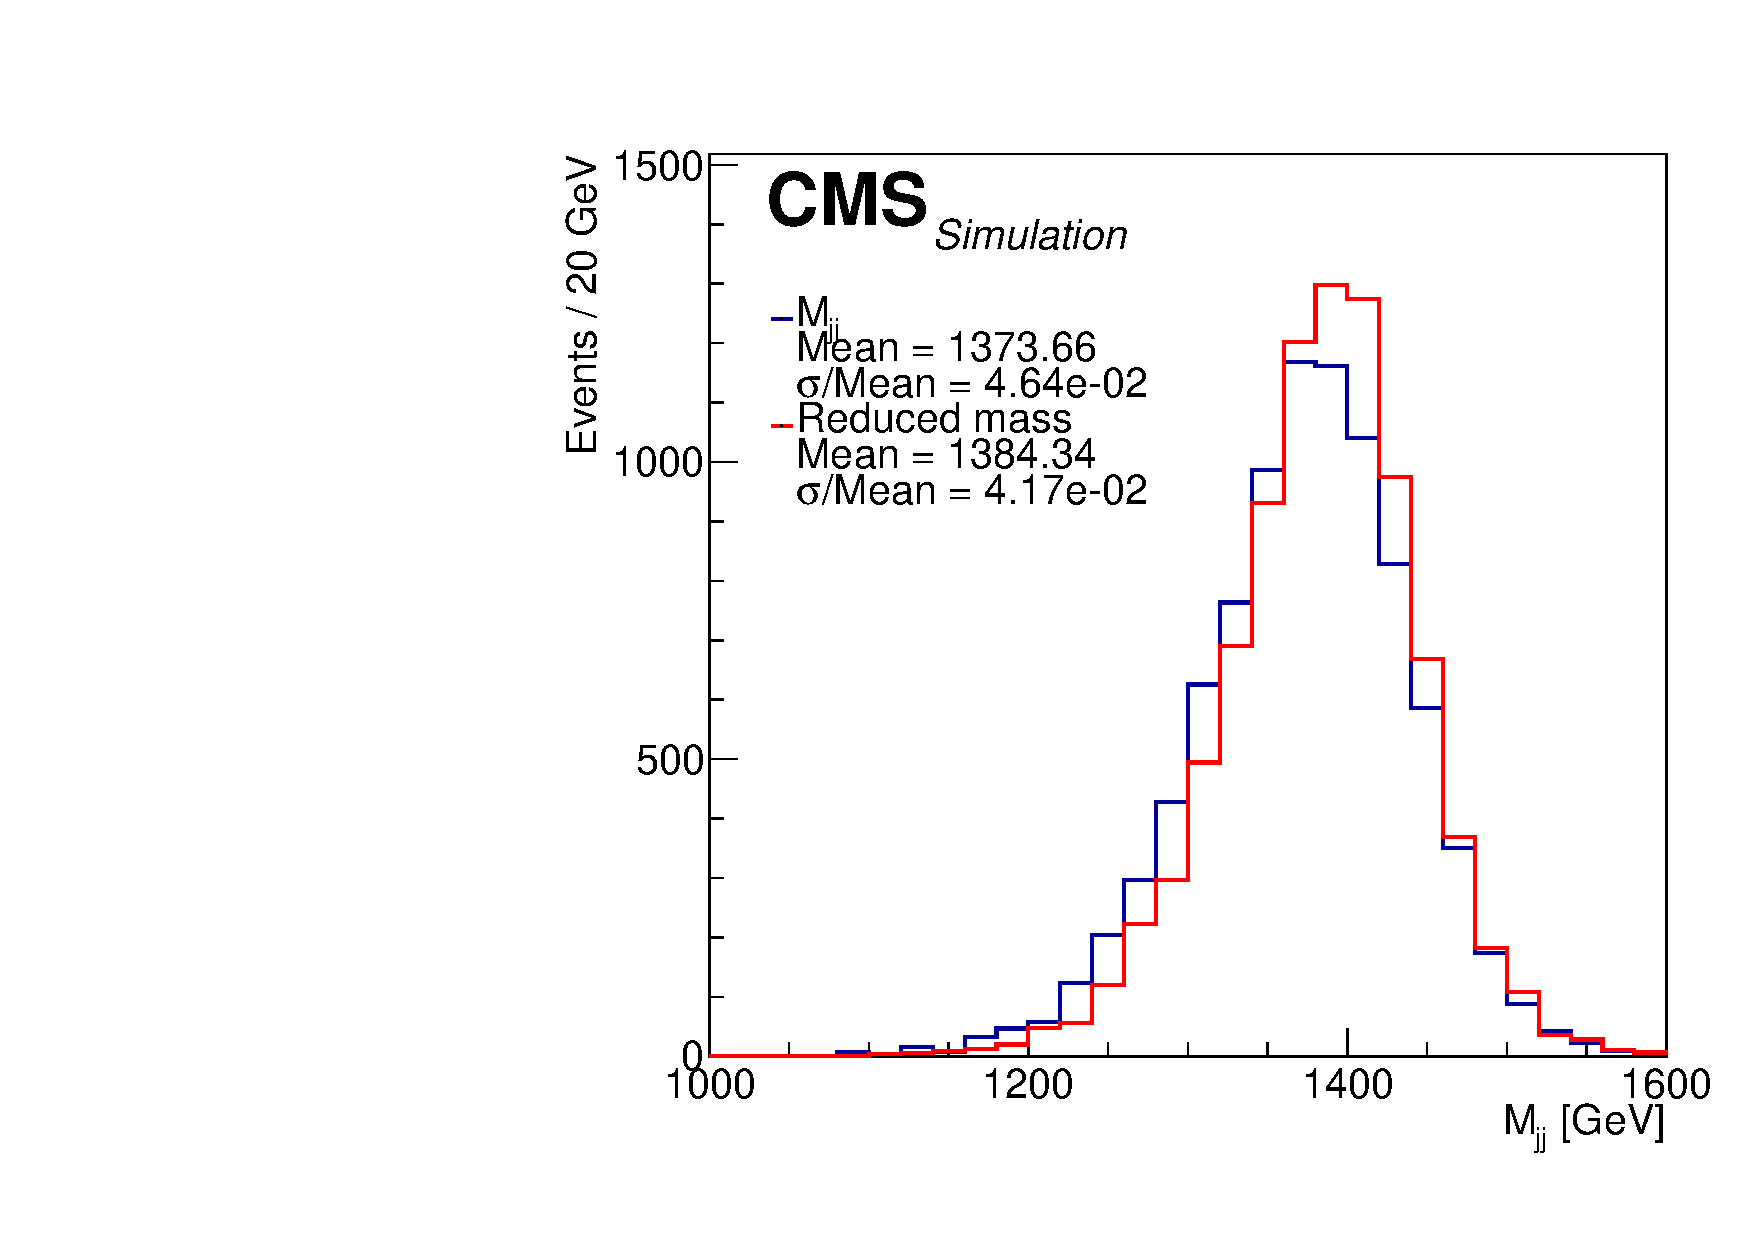
\includegraphics[width=0.5\textwidth]{Figures/red/1400.pdf} &
    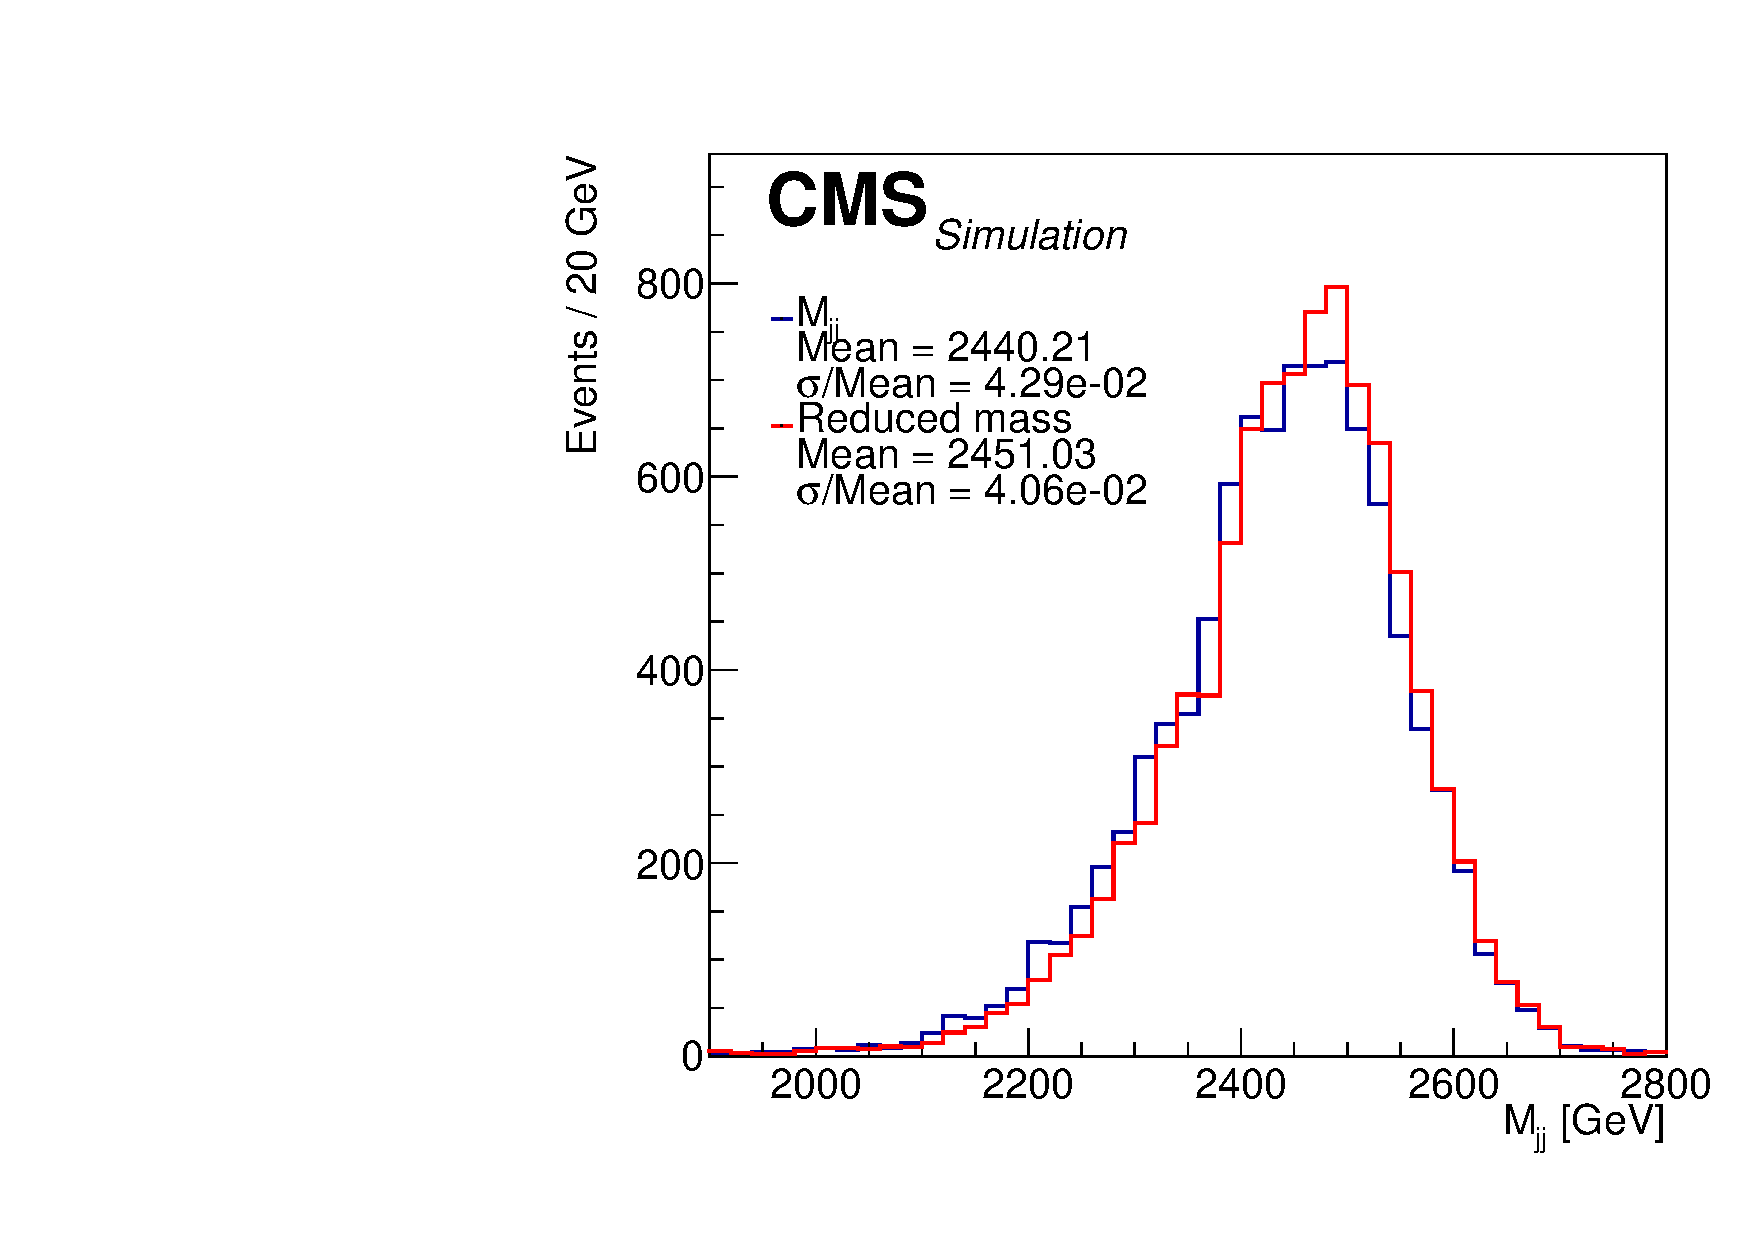
\includegraphics[width=0.5\textwidth]{Figures/red/2500.pdf} \\
    
  \end{tabular}
  \caption{The comparison of $M_{jj}$ and reduced mass distribution of bulk graviton $M_X$ = 1.4 (left) and 2.5 TeV (right). The mean and the $\sigma $/mean of a Gaussian fit to the distribution are shown.}
  \label{fig:hvt_brs}
\end{figure}

\subsection{Higgs Tagging Seletion} 

%http://xxx.lanl.gov/pdf/1402.2657v2
%CMS Collaboration, “Search for heavy resonances in the W/Z-tagged dijet mass spectrum at 13 TeV”, CMS Analysis Note CMS-AN-16-235, CERN, 2016.
%PUPPI soft-drop mass with W boson generator level correction & 105$<$ and $<$135 \\
The soft-drop procedure is inplemented to re-cluster the jet by removing soft contribution as follow\citep{Larkoski:2014wba}
\begin{itemize}
\item Deculster a targeted jet into two sub-jets.
\item Continue to decompose the sub-jets until the condition is achieved
\begin{equation} \label{eq5}
\begin{split}
\frac{min(p_{T1},p_{T2})}{p_{T1}+p_{T2}} > Z_{cut} \times (\frac{\Delta R_{12}}{R_0})^{\beta}, 
\end{split}
\end{equation}
where $R_0$ is the cone size of the original cluster algorithm, $p_T$ are the transverse momenta of two sub-jets, $\Delta R_{12}$ is the distance of two sub-jets in $\eta \phi$ space, and $Z_{cut}$ and $\beta $ are parameters. 
\item The unsplit singelet particle at the end will either be removed or remain preserved.
\end{itemize} 
If $\beta  >$ 0, the soft contribution is removed while remain a fraction of soft-collinear radiation. 
If $\beta  <$ 0, soft drop removes both soft and collinear radiation.
In CMS, the $Z_{cut}$ and $\beta $ are set 0.1 and zero respectively.
The difference between the peak of the distribution of mass of PUPPI soft-drop jets and the mass of physical Higgs boson is found\citep{CMS-AN-16-235}.
A Correction is applied to move the peak to the true phyiscal value. 
The ratio is derived by peak of the mass distribution of reconstructed jets in WW dijet Monte Carlo simulations to mass of true physical value.
The corrected PUPPI soft-drop mass of the first two leading jets are required between 105 and 135 GeV, which has been optimized.
 
%https://arxiv.org/abs/1011.2268
%https://arxiv.org/pdf/1108.2701
%https://arxiv.org/abs/1004.2489
%https://twiki.cern.ch/twiki/bin/view/CMS/JetWtagging#Working_points_and_scale_factors
%$\tau$21 & $<$ 0.55 \\
The ratio $\tau _N $ to $\tau _{N-1}$ is used as a discriminant to seperate the boosted events decaying into N particles from multi-jet events. $\tau _N $ is so-called "N-subjettiness" algorithm\citep{Thaler:2010tr,Thaler:2011gf,Stewart:2010tn}
\begin{equation} \label{eq6}
\begin{split}
\tau _N = \frac{1}{d_0} \sum\limits_{k}  p_{T,k} min \{ \Delta R_{1,k},\Delta R_{2,k},\cdots,\Delta R_{N,k} \} \\
d_0 = \sum\limits_{k}  p_{T,k} R_0,
\end{split}
\end{equation}
where k runs over the constituent particles in a given jet, $\Delta R_{jk}$ is the distance between particle j and k in $\eta \phi$ space, $R_0$ is the cone size of the original cluster algorithm. In the analysis, the boosted jets are decaying into two sub-jets, so $\tau _2 $ to $\tau _1$ ratio is used, and it is referred as $\tau _{21}$ in the following chapters.
The $\tau _{21}$ is required to be less than 0.55.  
The working point and simualtion-to-data scale factor is derived by JME POG\citep{WTagTWikiWPs}.

The double-b tagger is a multiple variable analysis discriminant used to identify b-flavor jets\citep{CMS-PAS-BTV-15-002}. Jets in multi-jet evetns and Higgs jets decaying into $b\bar{b}$ are used for training. Here lists out the input information:
\begin{itemize}
\item The first four impact paramters to its uncertainty values ordered from the largest to the smallest.
\item The  N-subjettiness axes referred as $\tau $-axes use the information of N-subjettiness
\item The first two impact parameters to its uncertainty values of $\tau $-axes ordered from the largest to the smallest.
\item The meausured significance of impact parameters of the first two tracks whose mass of secondary vertex is above buttom quark threshold.
\item The number of secondary verteces of the jet.
\item The significance of two dimenisional distance between the primary vertex and the secondary vertex and flight distance of the secondary vertex with smallest three dimenisional distance uncertainty for each $\tau $-axes.
\item $\Delta R$ of the two secondary verteces with smallest three dimenisional distance uncertainty for each $\tau $-axes.
\item The $\tau $-axis of the two secondary verteces with smallest three dimenisional distance uncertainty for each $\tau $-axes.
\item The sum of the mass of the secondary verteces associated to the $\tau $-axis for each $\tau $-axes.
\item The sum of energy of secondary verteces associated to the $\tau $-axis for each $\tau $-axes.
\item The relative pseudorapidity of three tracks of leading secondary vertex with respect to their $\tau $-axis for each $\tau $-axes.
\item The sum of energy of all tracks in the AK8 jet.
\item The z variable, defined as: 
\begin{equation} \label{eq7}
\begin{split}
z = \Delta R (SV_0, SV_1) \times \frac{p_{T,SV_1}}{m(SV_0,SV_1)}, 
\end{split}
\end{equation}
where $SV_0$ and $SV_1$ are the secondary verteces with the smallest 3D flight distance uncertainty.
\end{itemize} 
%https://cds.cern.ch/record/2195743
%https://twiki.cern.ch/twiki/bin/viewauth/CMS/BtagRecommendation80XReReco
The double-b working points and simualtion-to-data scale factor is derived by BTV POG\citep{BtagRecommendation80XReReco}.
The analysis is seperated into two catgory with two Higgs jets in the events either both passing loose working point ($>$ 0.3) or both passing tight working point ($>$ 0.8), which are referred as LL and TT categories respectively. The events sit in TT region will be excluded from LL region to make two categories orthogonal.
%double-b tagger & $>$0.3 or $>$0.8 \\



\section{Triggers} \label{Triggers}
Since the final state includes di-Higgs jets, the triggers are selected considering the requirements on the scale sum of the energy of external partons $H_T$, |$\Delta \eta $(the first two leading jets)|, M$_{jj}$, $p_T$, the groomed mass of the jets, and double-b tagger. PFHT900 is used to supplement the inefficiency of PFHT800 in period H of data taking.
\begin{table}[h!]
  \begin{center}
    \begin{tabular}{l}
    Triggers \\
    \hline
    HLT$\_$PFHT800 \\
    HLT$\_$PFHT900 \\
    HLT$\_$PFHT650$\_$WideJetMJJ900DEtaJJ1p5 \\
    HLT$\_$AK8PFJet360$\_$TrimMass30 \\
    HLT$\_$AK8DiPFJet280$\_$200$\_$TrimMass30$\_$BTagCSV$\_$p20 \\
    HLT$\_$AK8PFHT650$\_$TrimR0p1PT0p03Mass50 \\
    \hline
    \end{tabular}
  \end{center}

  \caption{List of Triggers applied in the analysis.}
\end{table} 

\begin{table}[h!]
  \begin{center}
    \begin{tabular}{ll}
    Selection & Requirement \\
    \hline
    Number of good vertex & $>$ 1 \\
    MET Filters & AND of all filters\\
	Trigger & OR of all triggers\\
	Lepton veto & one tight-tagged or two loose-tagged \\
    $p_{T}$ of AK8 jets & $>$ 300GeV \\
	|$\eta$| of AK8 jets & $<$ 2.4 \\
	Tight LepVeto jet ID & pass \\
	|$\Delta \eta $ (two AK8 jets) | & $<$ 1.3 \\
	Reduce mass & $>$ 750 GeV \\
	corrected PUPPI soft-drop mass & 105 $<$ and $<$ 135 \\
	$\tau _{21}$ & $<$ 0.55 \\
	double-b tagger & $>$ 0.3 (LL) or $>$ 0.8 (TT)\\
	\hline
    \end{tabular}
  \end{center}

  \caption{List of all selection in the analysis.}
\end{table} 

\begin{table}[h!]
  \begin{center}
    \begin{tabular}{lllllllllll}
    $M_X$ & Trig. & Jet $p_T$, $\eta$ & Veto$_{lep}$ & $\Delta \eta$ & Lepton & $\tau _{21}$ & $M_{AK8}$ & $M^{red}_{jj}$ & LL & TT\\
    \hline
750 & 0.432 & 0.248 & 0.247 & 0.213 & 0.213 & 0.093 & 0.029 & 0.024 & 0.016 & 0.009 \\
800 & 0.547 & 0.367 & 0.367 & 0.327 & 0.326 & 0.152 & 0.051 & 0.050 & 0.036 & 0.021 \\
900 & 0.693 & 0.552 & 0.552 & 0.487 & 0.485 & 0.245 & 0.083 & 0.083 & 0.061 & 0.033 \\
1000 & 0.772 & 0.666 & 0.666 & 0.552 & 0.550 & 0.296 & 0.101 & 0.101 & 0.075 & 0.041 \\
1200 & 0.859 & 0.792 & 0.792 & 0.585 & 0.584 & 0.335 & 0.116 & 0.116 & 0.084 & 0.044 \\
1400 & 0.902 & 0.854 & 0.854 & 0.591 & 0.590 & 0.355 & 0.123 & 0.123 & 0.087 & 0.044 \\
1600 & 0.928 & 0.890 & 0.889 & 0.592 & 0.591 & 0.358 & 0.124 & 0.124 & 0.086 & 0.041 \\
1800 & 0.946 & 0.913 & 0.913 & 0.595 & 0.594 & 0.365 & 0.124 & 0.124 & 0.082 & 0.036 \\
2000 & 0.957 & 0.931 & 0.931 & 0.598 & 0.598 & 0.365 & 0.127 & 0.127 & 0.081 & 0.036 \\
2500 & 0.975 & 0.956 & 0.955 & 0.596 & 0.595 & 0.367 & 0.125 & 0.125 & 0.076 & 0.030 \\
3000 & 0.981 & 0.966 & 0.965 & 0.589 & 0.589 & 0.357 & 0.123 & 0.123 & 0.068 & 0.022 \\
3500 & 0.987 & 0.973 & 0.972 & 0.582 & 0.582 & 0.349 & 0.116 & 0.116 & 0.059 & 0.018 \\
4500 & 0.991 & 0.977 & 0.976 & 0.579 & 0.578 & 0.334 & 0.103 & 0.103 & 0.044 & 0.010 \\
\hline
    \end{tabular}
  \end{center}
	
  \caption{The cut flow of all $M_X$ (GeV) of spin-0 radion.}
\end{table} 

\begin{table}[h!]
  \begin{center}
    \begin{tabular}{lllllllllll}
    $M_X$ & Trig. & Jet $p_T$, $\eta$ & Jet ID & $\Delta \eta$ & Veto$_{lep}$ & $\tau _{21}$ & $M_{AK8}$ & $M^{red}_{jj}$ & LL & TT\\
    \hline
    750 & 0.610 & 0.368 & 0.368 & 0.331 & 0.330 & 0.149 & 0.049 & 0.039 & 0.027 & 0.015 \\
	800 & 0.758 & 0.541 & 0.541 & 0.503 & 0.502 & 0.237 & 0.080 & 0.079 & 0.057 & 0.032 \\
	900 & 0.903 & 0.772 & 0.771 & 0.716 & 0.715 & 0.371 & 0.125 & 0.124 & 0.092 & 0.051 \\
	1000 & 0.958 & 0.885 & 0.885 & 0.801 & 0.799 & 0.434 & 0.151 & 0.151 & 0.111 & 0.062 \\
1200 & 0.988 & 0.962 & 0.961 & 0.843 & 0.842 & 0.499 & 0.178 & 0.178 & 0.129 & 0.068 \\
1400 & 0.996 & 0.984 & 0.983 & 0.854 & 0.853 & 0.524 & 0.182 & 0.182 & 0.129 & 0.064 \\
1600 & 0.998 & 0.993 & 0.993 & 0.858 & 0.857 & 0.532 & 0.186 & 0.186 & 0.128 & 0.061 \\
1800 & 0.999 & 0.996 & 0.996 & 0.864 & 0.863 & 0.543 & 0.193 & 0.193 & 0.130 & 0.059 \\
2000 & 1.000 & 0.998 & 0.998 & 0.861 & 0.860 & 0.541 & 0.190 & 0.190 & 0.123 & 0.054 \\
2500 & 1.000 & 0.999 & 0.999 & 0.862 & 0.862 & 0.538 & 0.188 & 0.188 & 0.113 & 0.044 \\
3000 & 1.000 & 1.000 & 0.999 & 0.865 & 0.865 & 0.530 & 0.186 & 0.186 & 0.102 & 0.034 \\
4000 & 1.000 & 1.000 & 0.999 & 0.861 & 0.861 & 0.505 & 0.166 & 0.166 & 0.078 & 0.021 \\
4500 & 1.000 & 1.000 & 0.999 & 0.859 & 0.858 & 0.502 & 0.156 & 0.156 & 0.065 & 0.016 \\
\hline
    \end{tabular}
  \end{center}
	
  \caption{The cut flow of all $M_X$ (GeV) of spin-2 bulk graviton.}
\end{table} 



\section{Simulation Distribution} 
In the section, distribution of Monte Carlo simulations of signal and background will be shown to demonstrate the discrimination of each variables of the seletion. For each distribution, all selection described in previous section is required except the variable itself and double-b tagger discriminant. The cross section of every signal is set to 20 pb. The numbers of events of signal and of background are normalized to same luminosity of data of 35.9fb$^{-1}$. Multi-jet events are added up by samples of different $H_T$ section listed in table 3.4, and seperated into four categories summarized in the table 3.10.  Besides, the cross sections at leading order of multi-jet events are multiplied by a factor about 0.7 to modify them closer to the value of next leading order.

\begin{table}[h!]
  \begin{center}
    \begin{tabular}{lll}
    category & hadron flavor of AK8 jets & hadron flavor of subjets \\
    \hline
    bb & 5 & 5 (both) \\
    b & 5 & 5 (only one) \\
    cc/c & 4 & 4 (at least one) \\
    light & all remaining & all remaining \\
	\hline
    \end{tabular}
  \end{center}

  \caption{List of categorization of multijet events.}
\end{table} 

\begin{figure}[t]
  \centering
  \begin{tabular}{cc}
    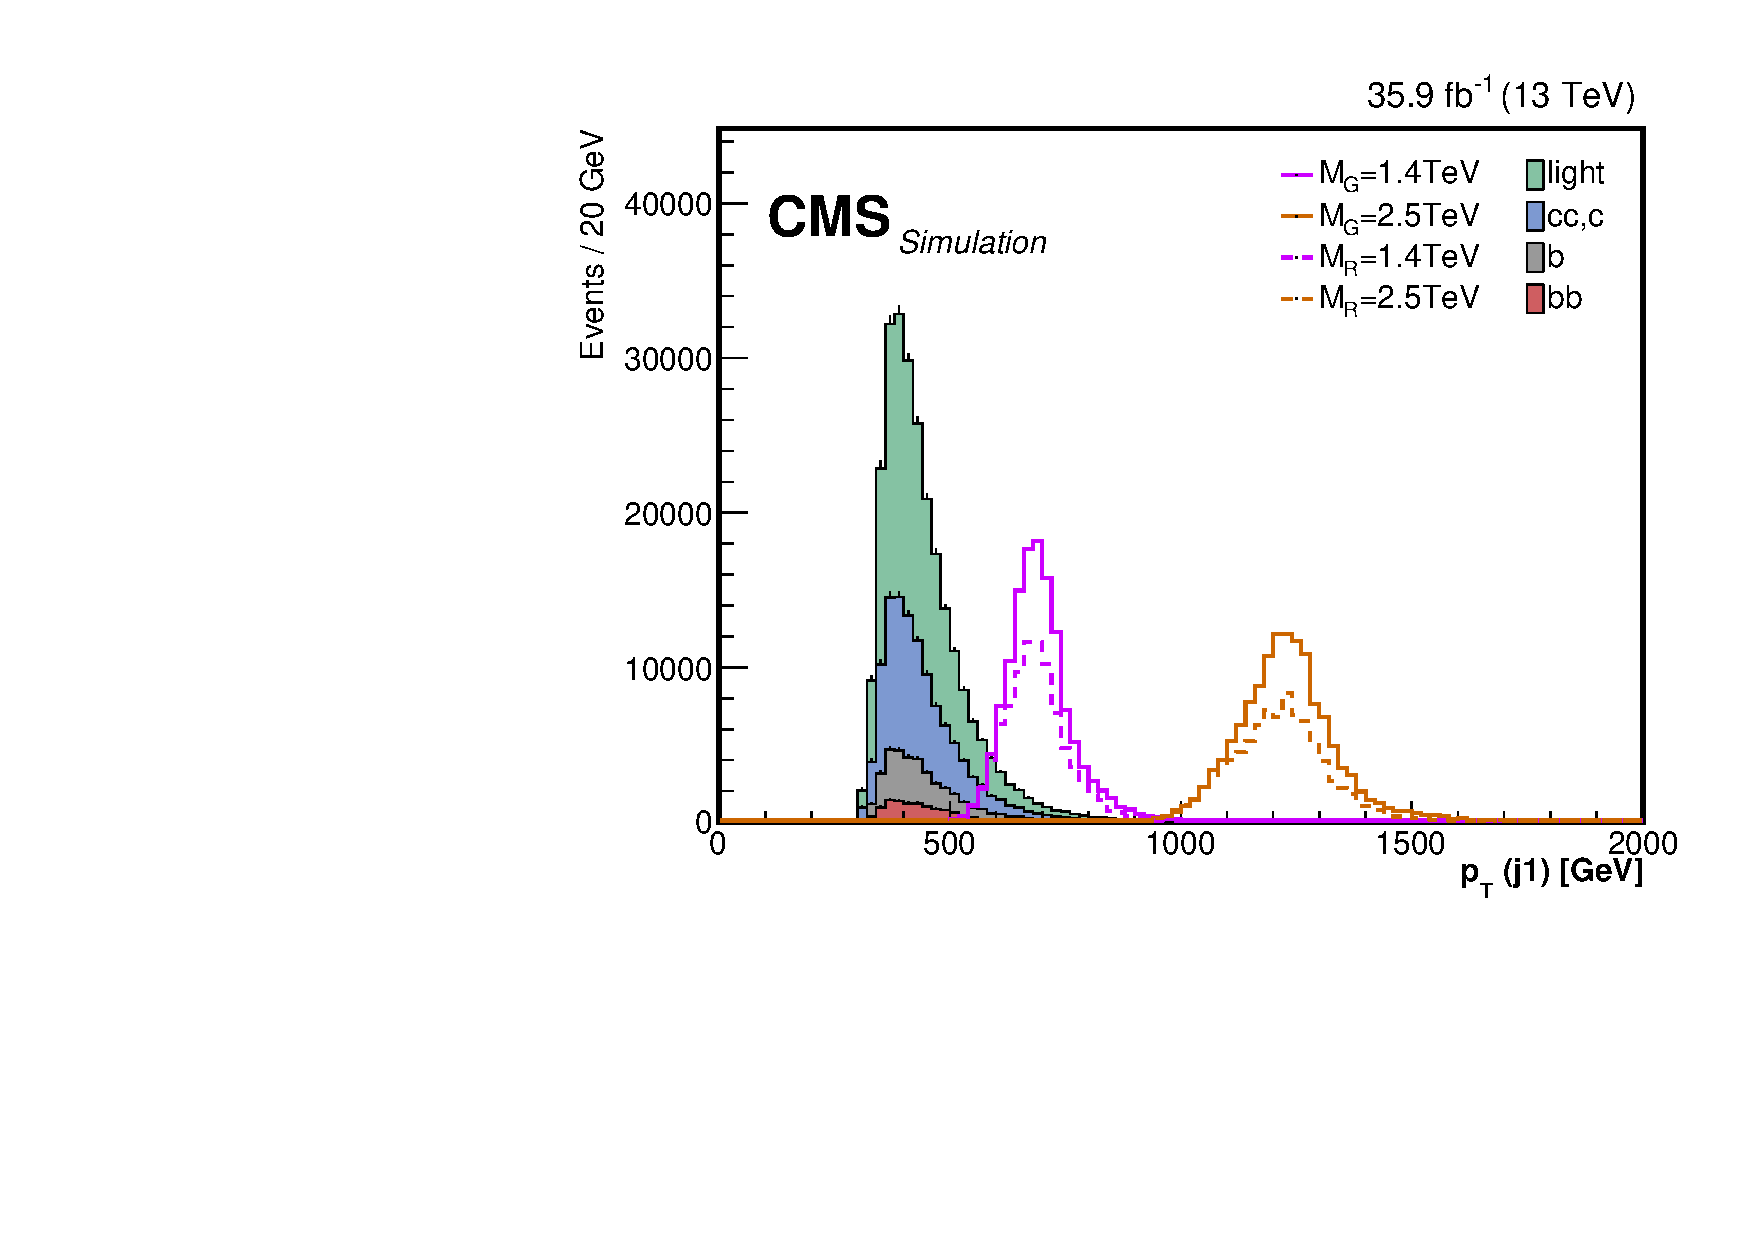
\includegraphics[width=0.5\textwidth]{Figures/MC_N1/pt_j0.pdf} &
    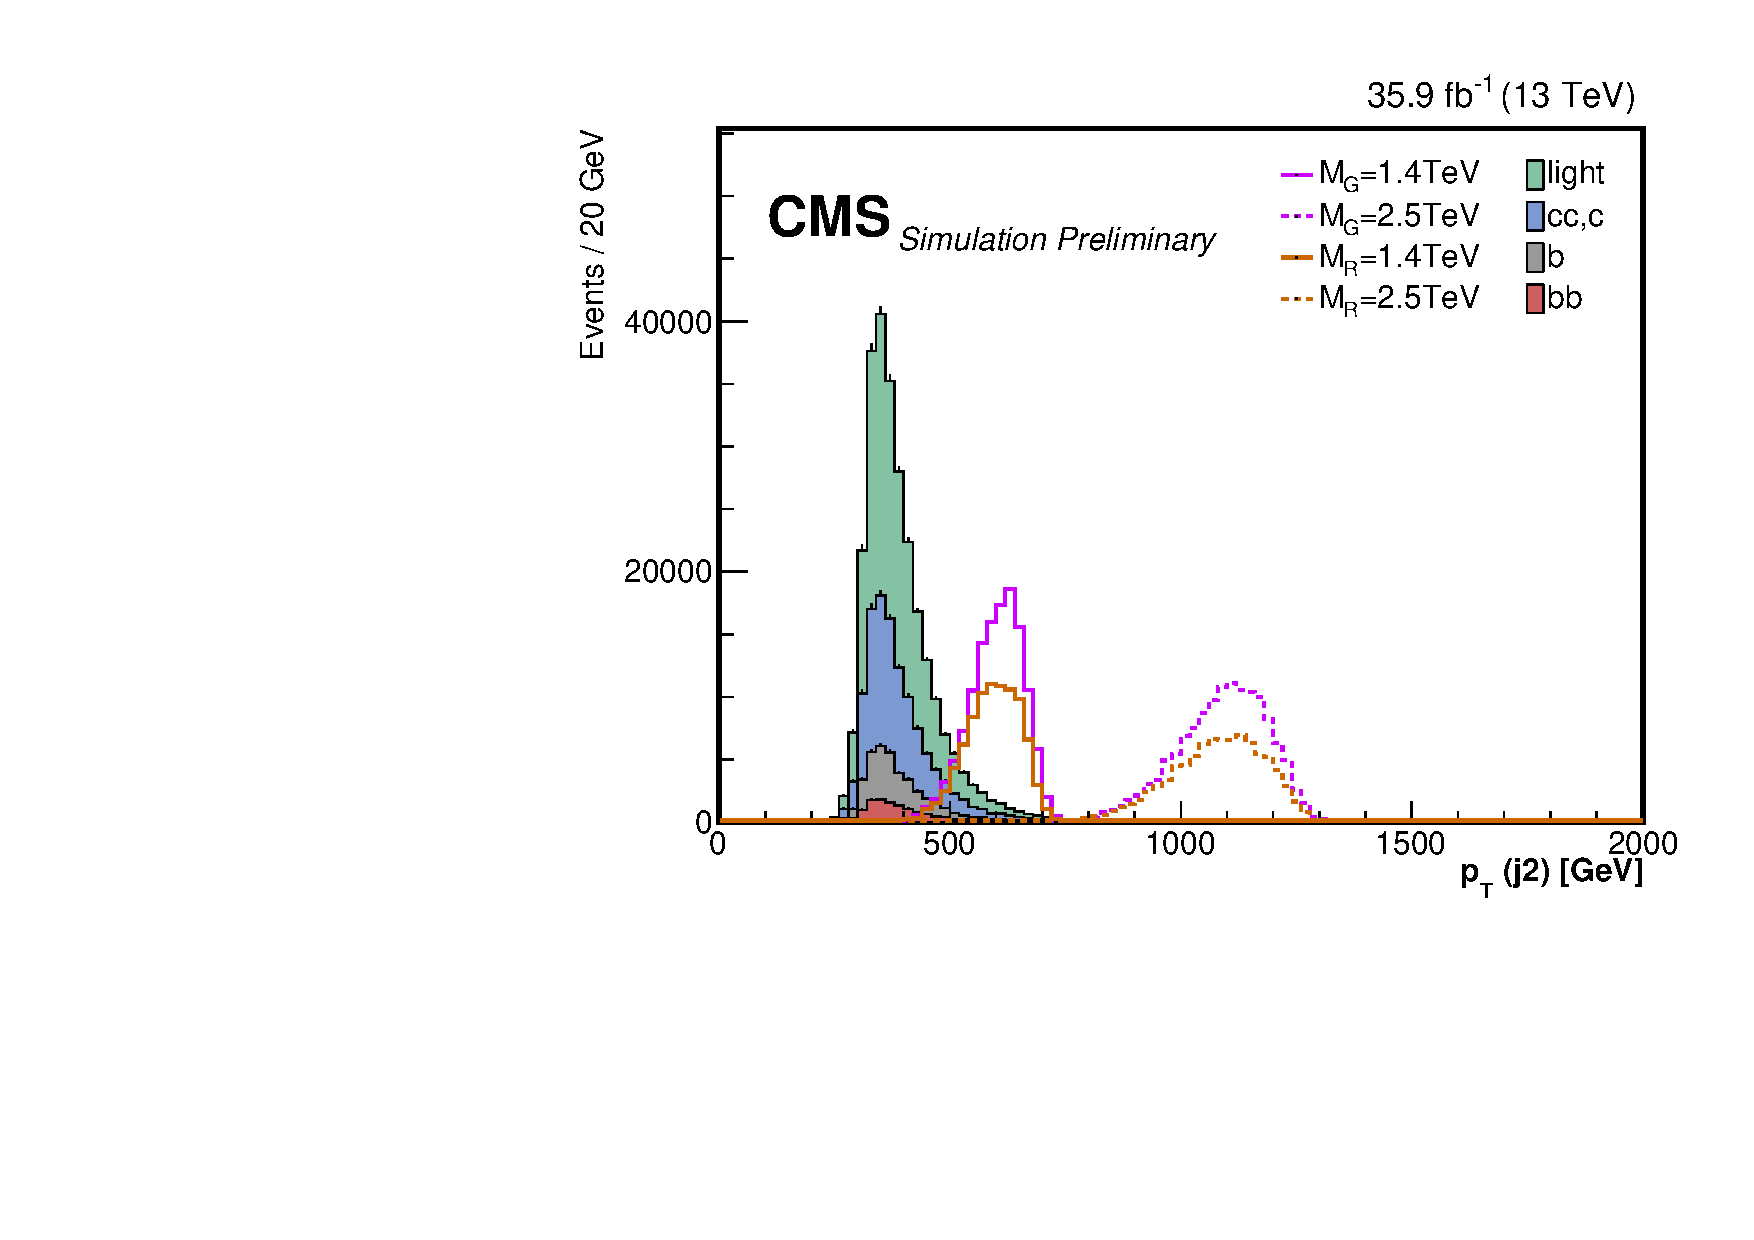
\includegraphics[width=0.5\textwidth]{Figures/MC_N1/pt_j1.pdf} \\
     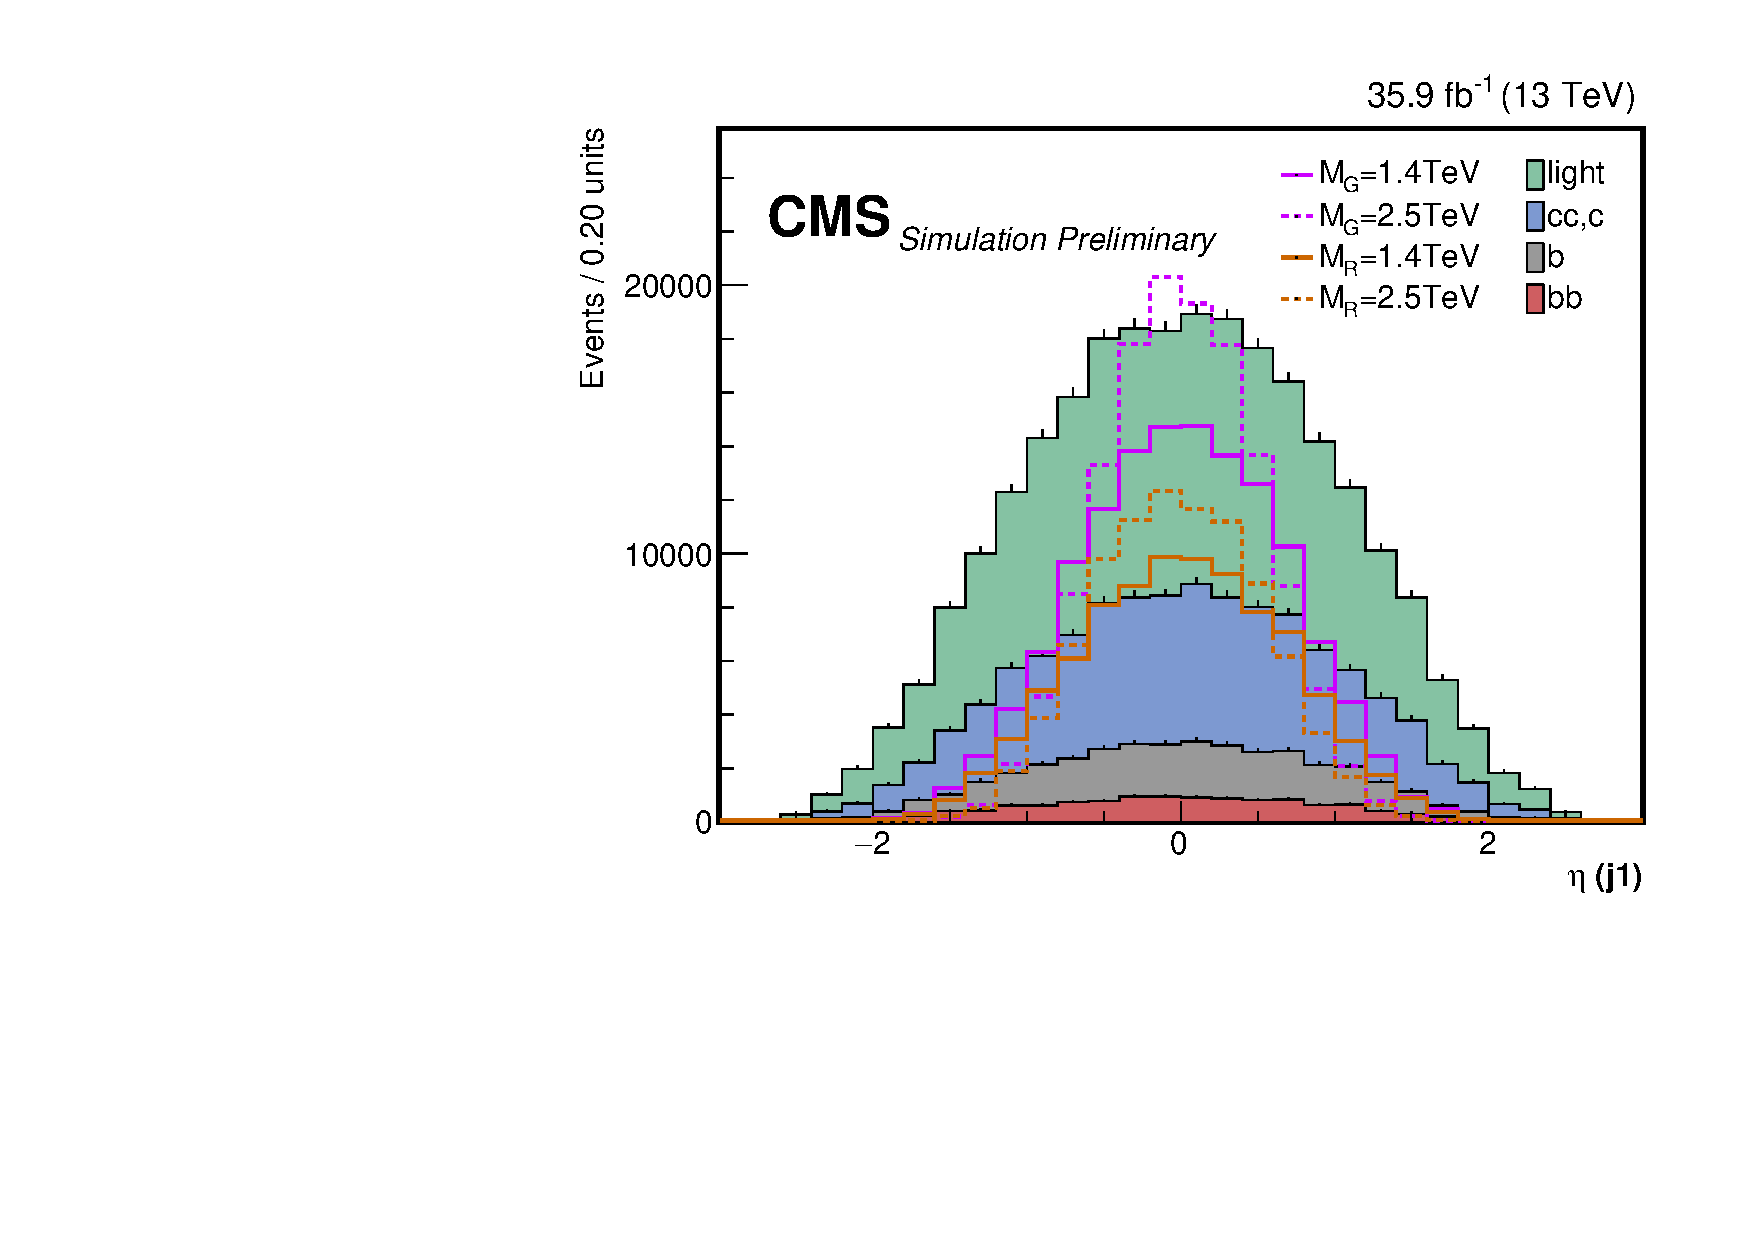
\includegraphics[width=0.5\textwidth]{Figures/MC_N1/eta_j0.pdf} &
    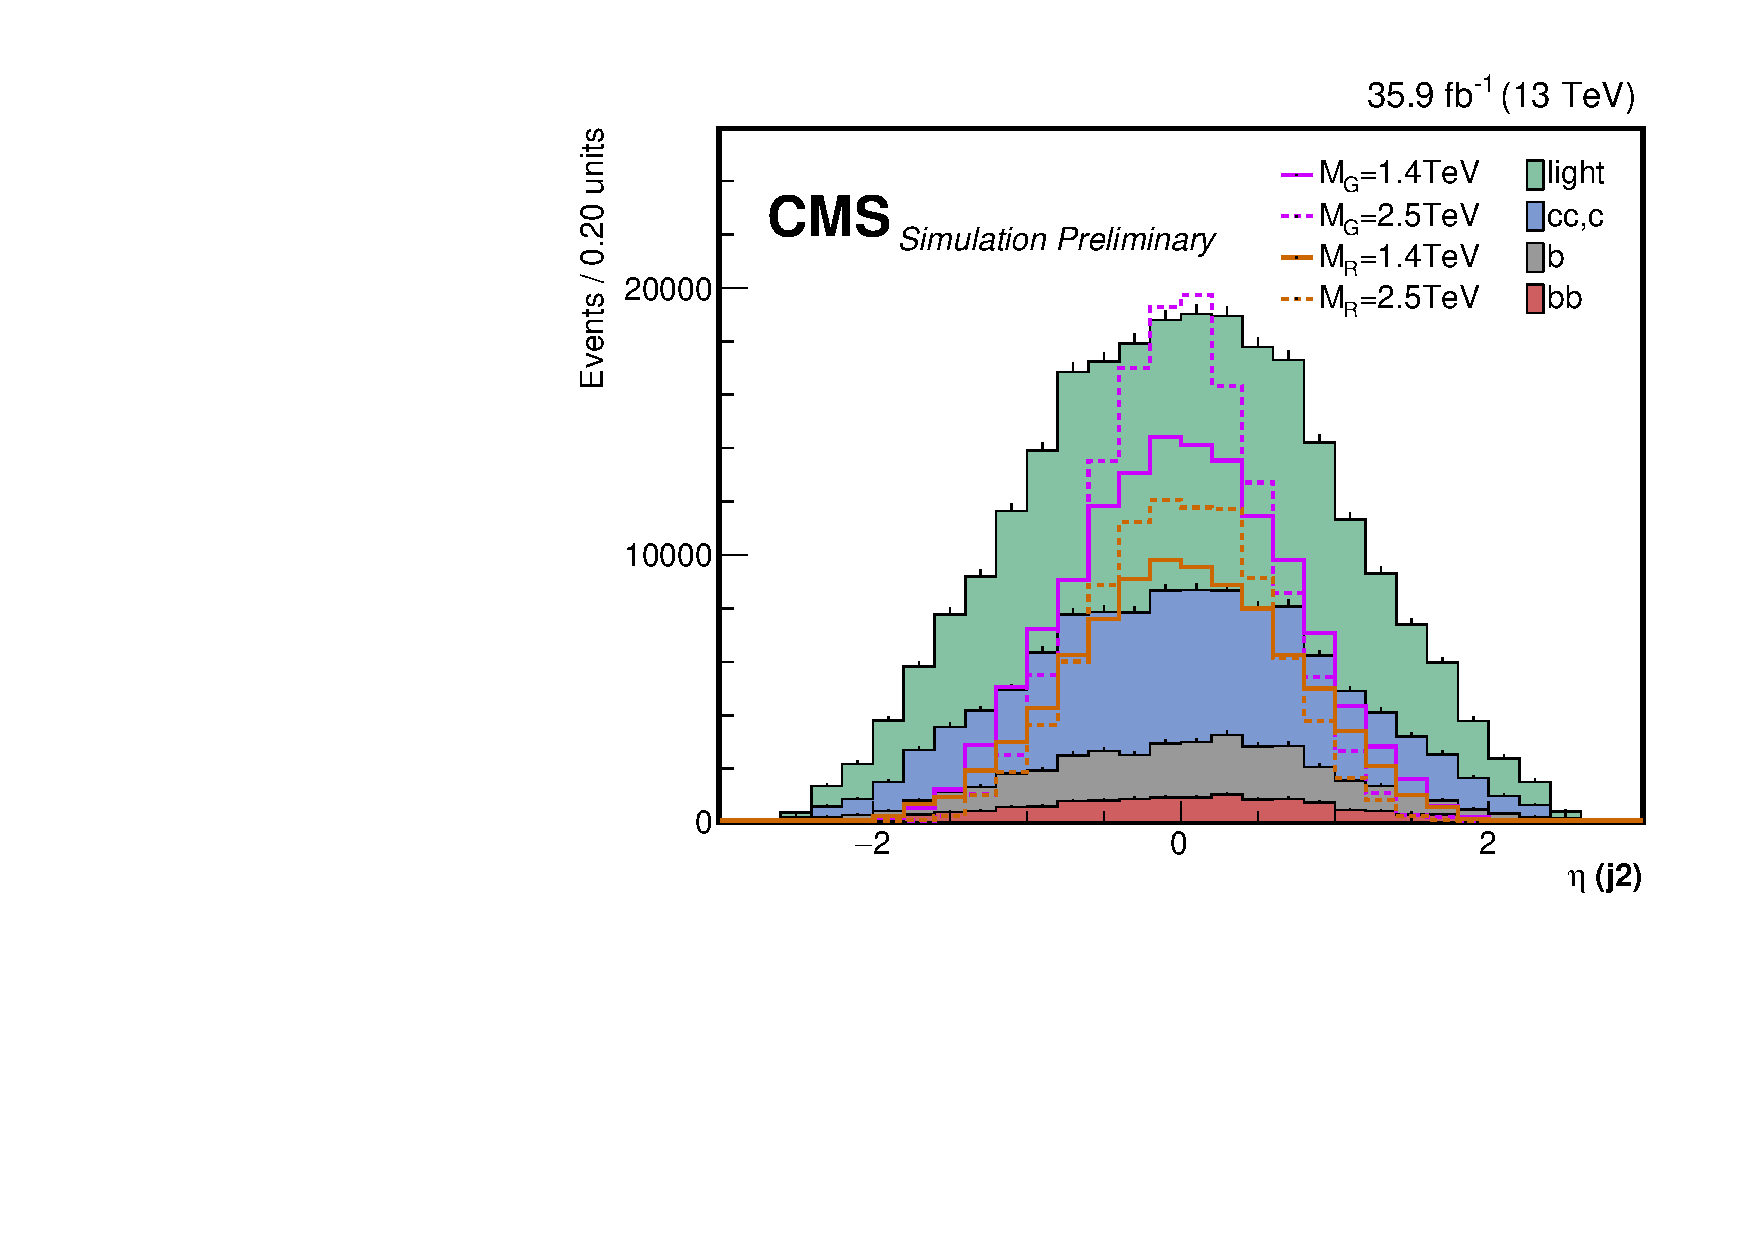
\includegraphics[width=0.5\textwidth]{Figures/MC_N1/eta_j1.pdf} \\
     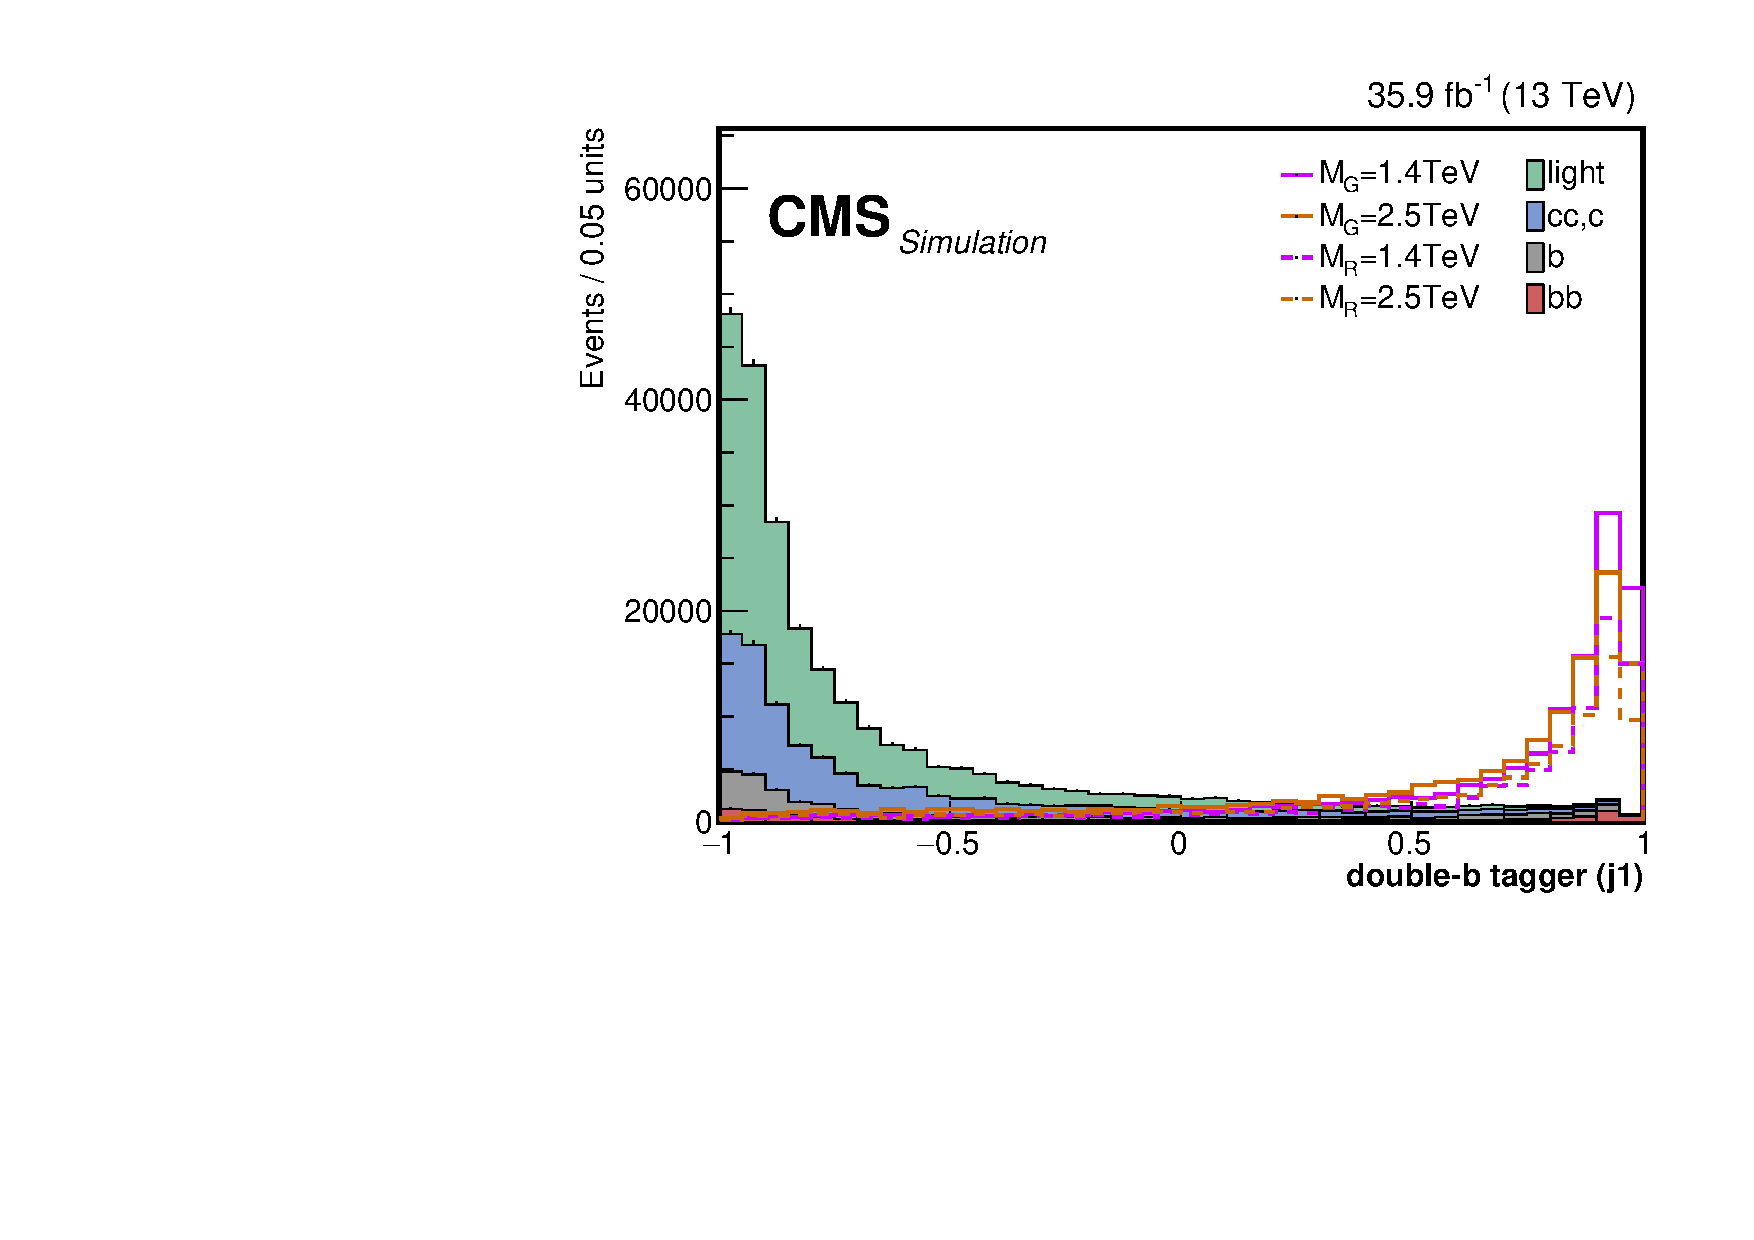
\includegraphics[width=0.5\textwidth]{Figures/MC_N1/doubleSV_j0.pdf} &
    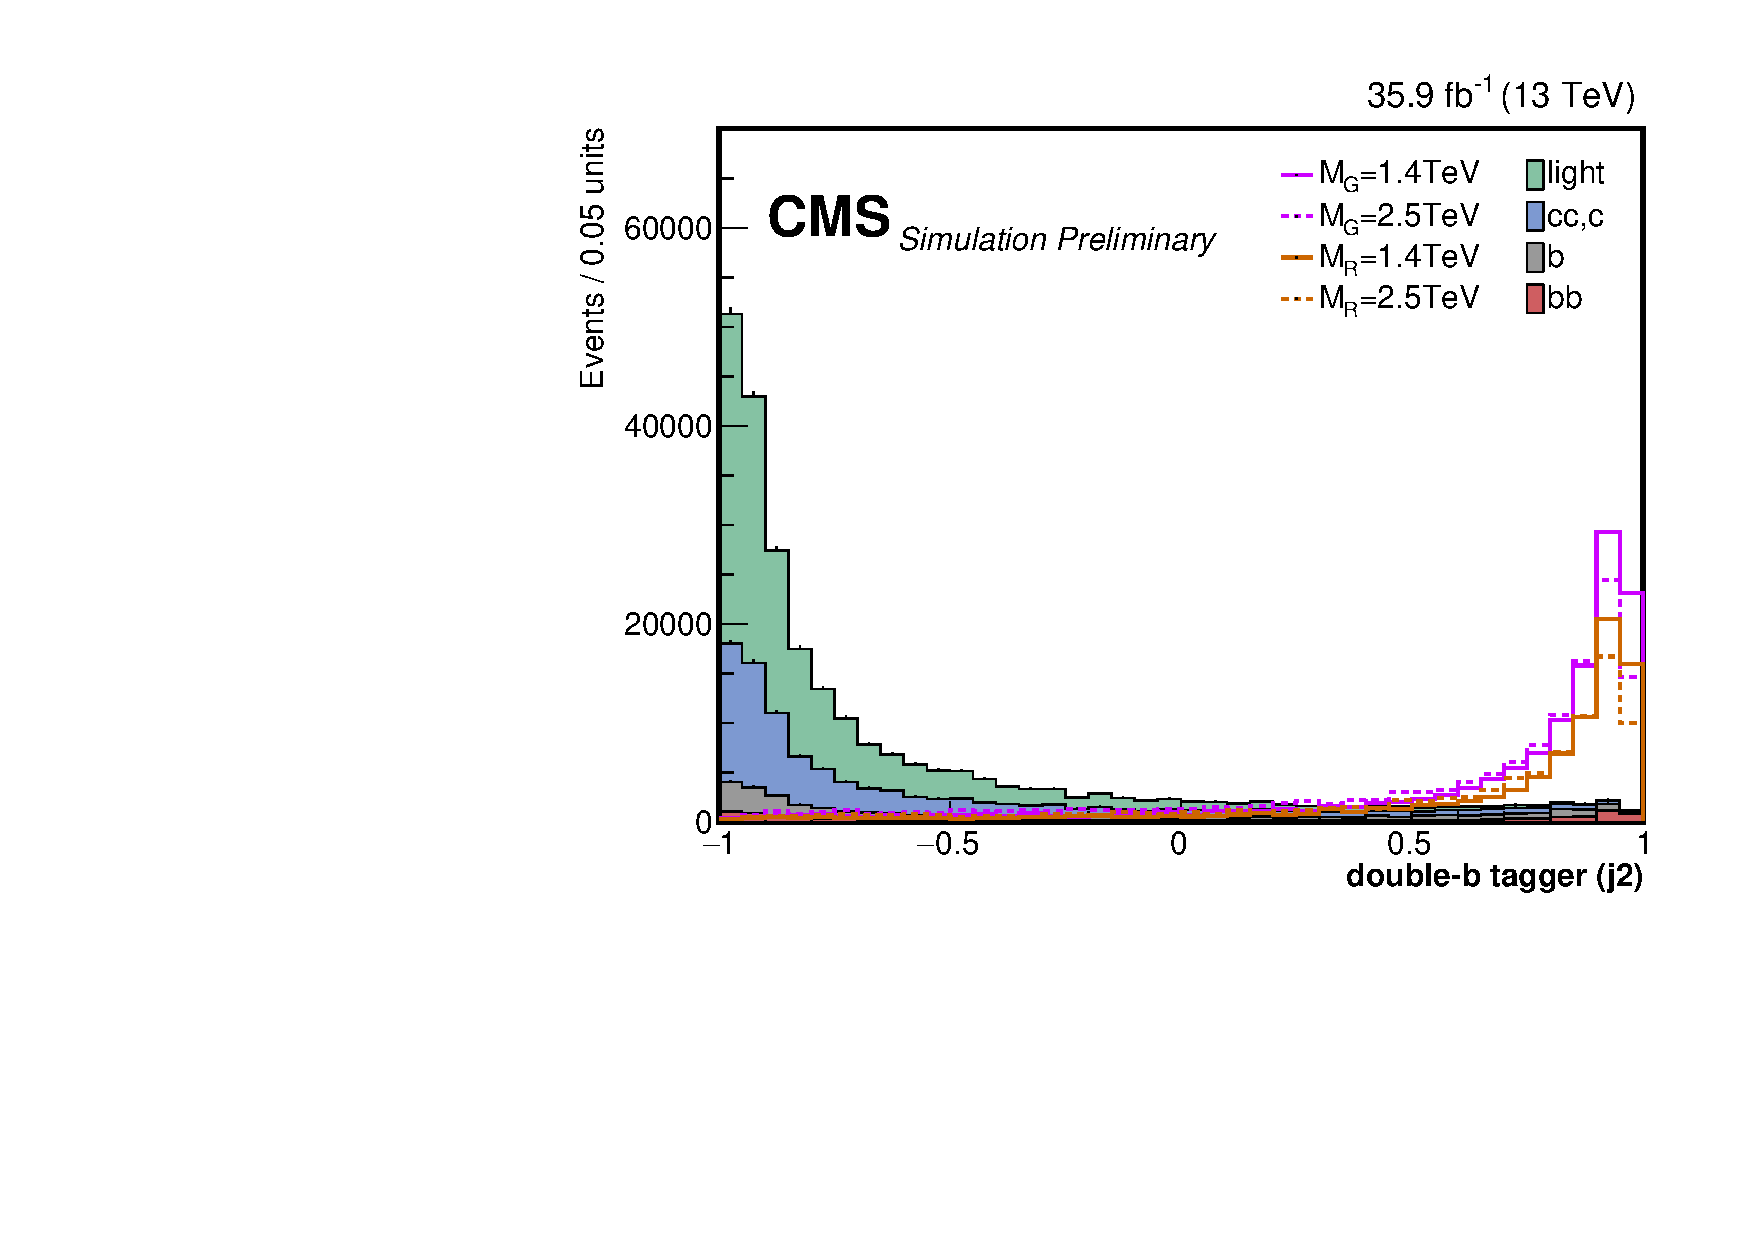
\includegraphics[width=0.5\textwidth]{Figures/MC_N1/doubleSV_j1.pdf} \\
  \end{tabular}
  \caption{The comparison of signal and background. The signals of $M_{X}$ = 1.4 TeV and 2.5 TeV from both models are shown. The cross section is set to 20 pb in the figures. Multi-jet events are seperated into four categories summarized in the table 3.10. From top to buttom are the comparison of $p_{T}$, $\eta $, and double-b tagger of leading (left) and next leading (right) AK8 jet.}
  \label{fig:hvt_brs}
\end{figure}

\begin{figure}[t]
  \centering
  \begin{tabular}{cc}
    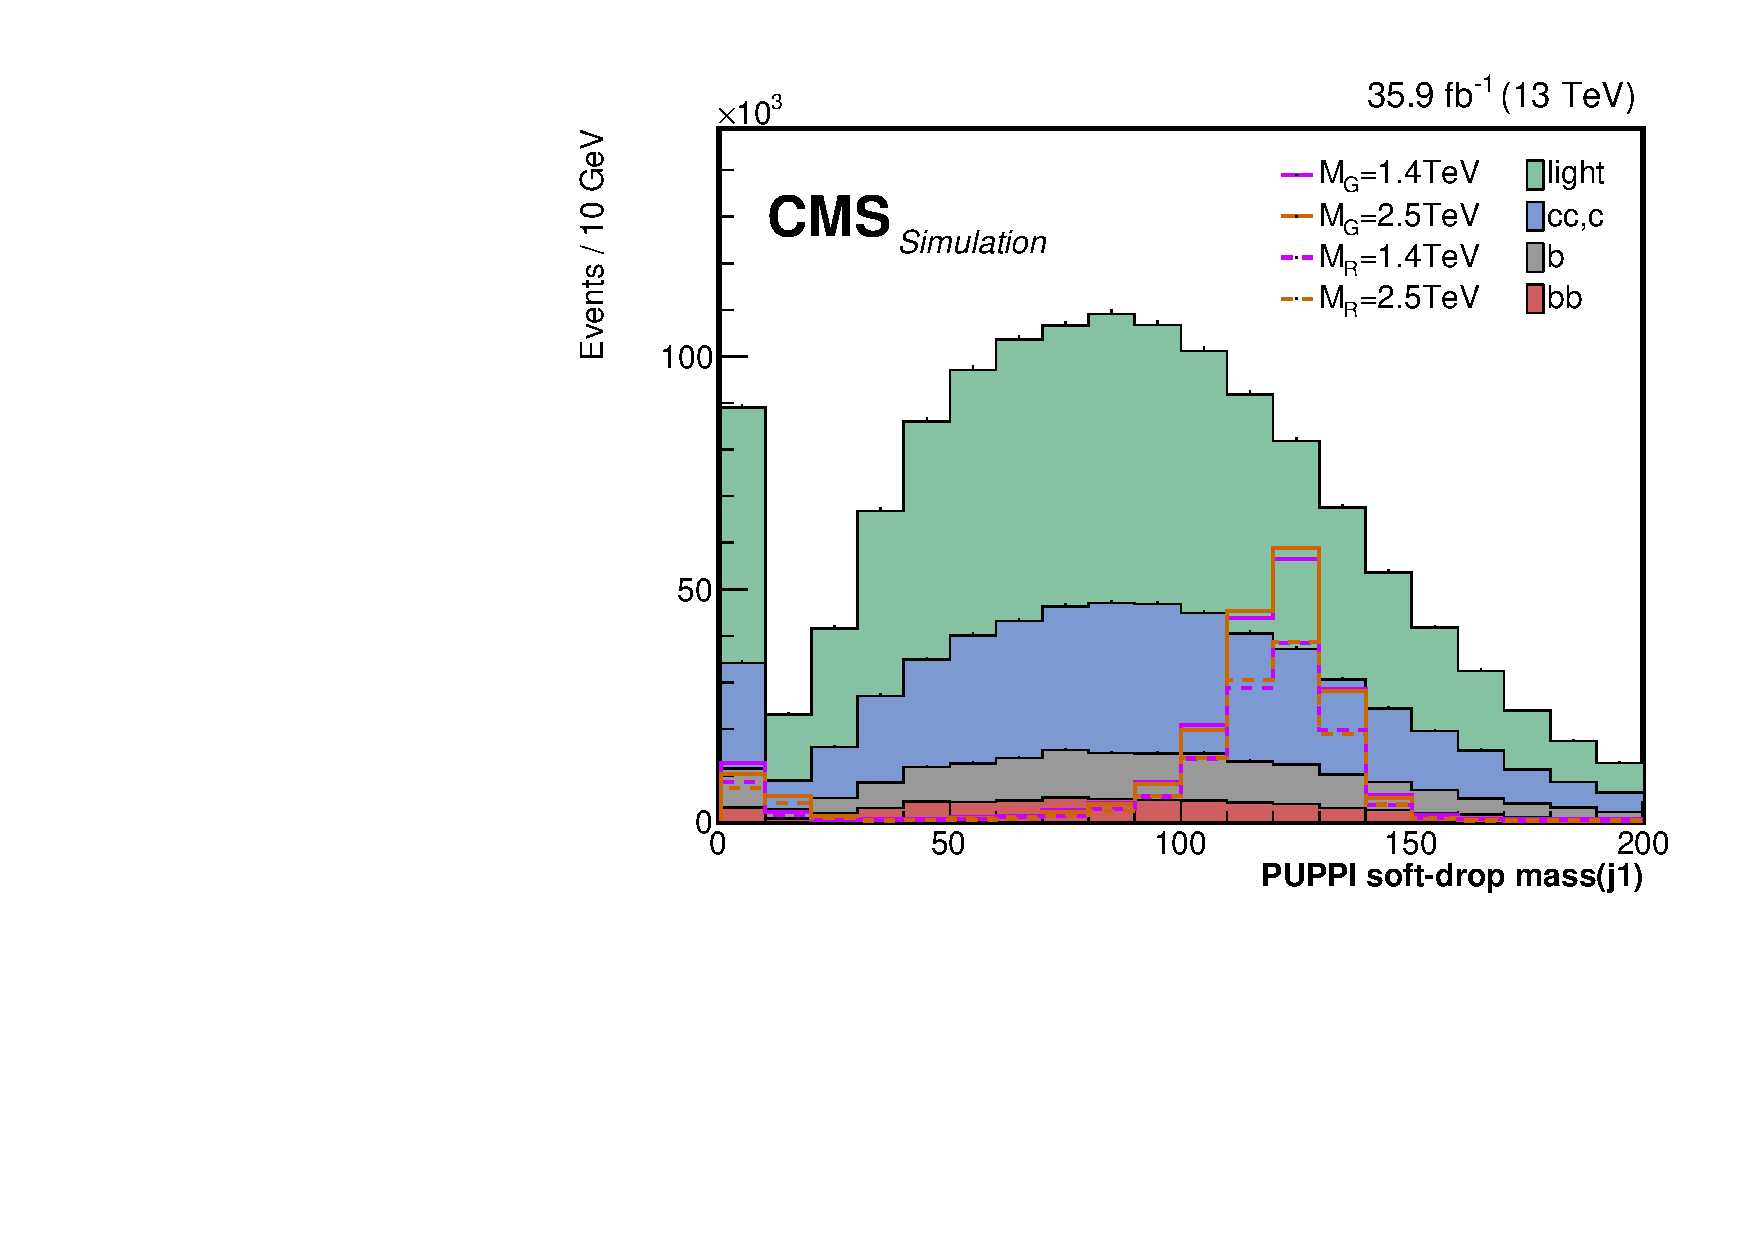
\includegraphics[width=0.5\textwidth]{Figures/MC_N1/puppiSDMassThea_j0.pdf} &
    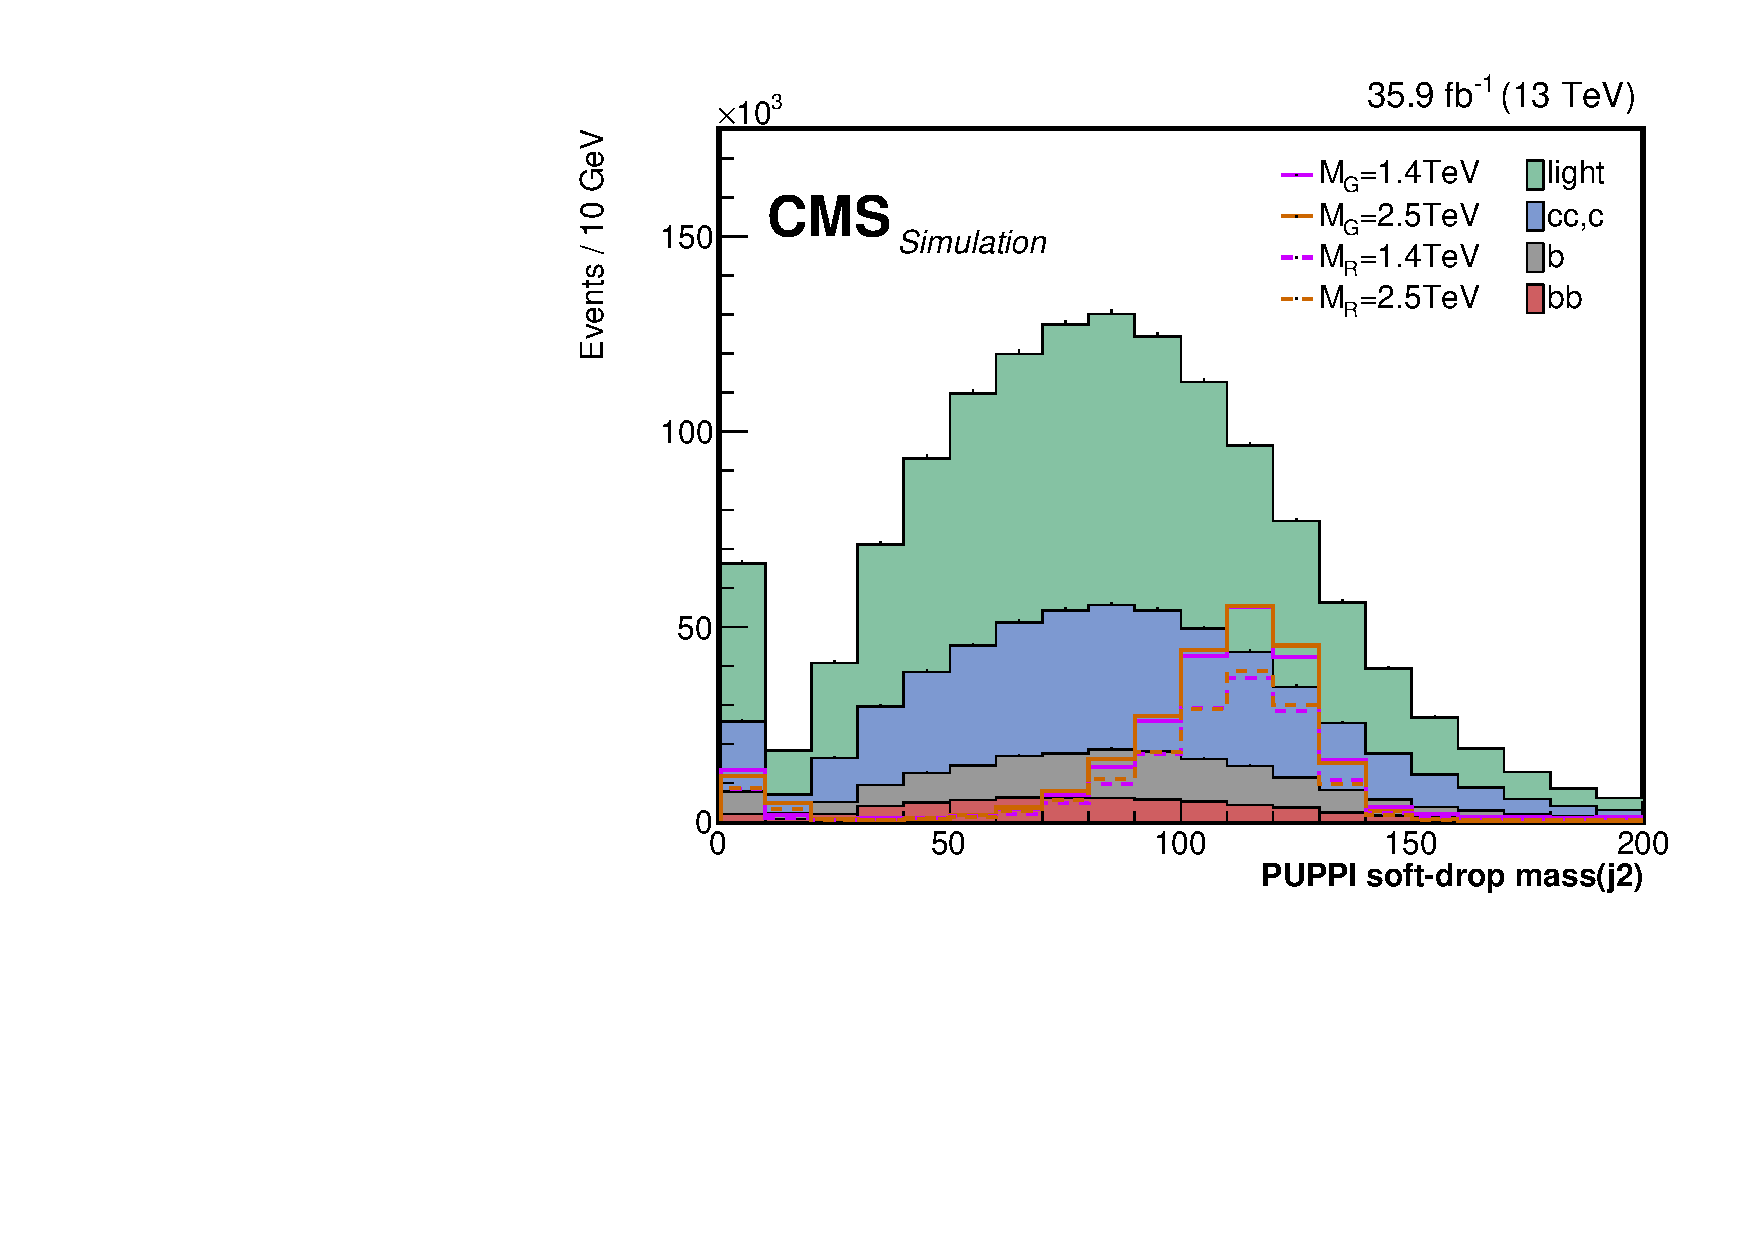
\includegraphics[width=0.5\textwidth]{Figures/MC_N1/puppiSDMassThea_j1.pdf} \\
     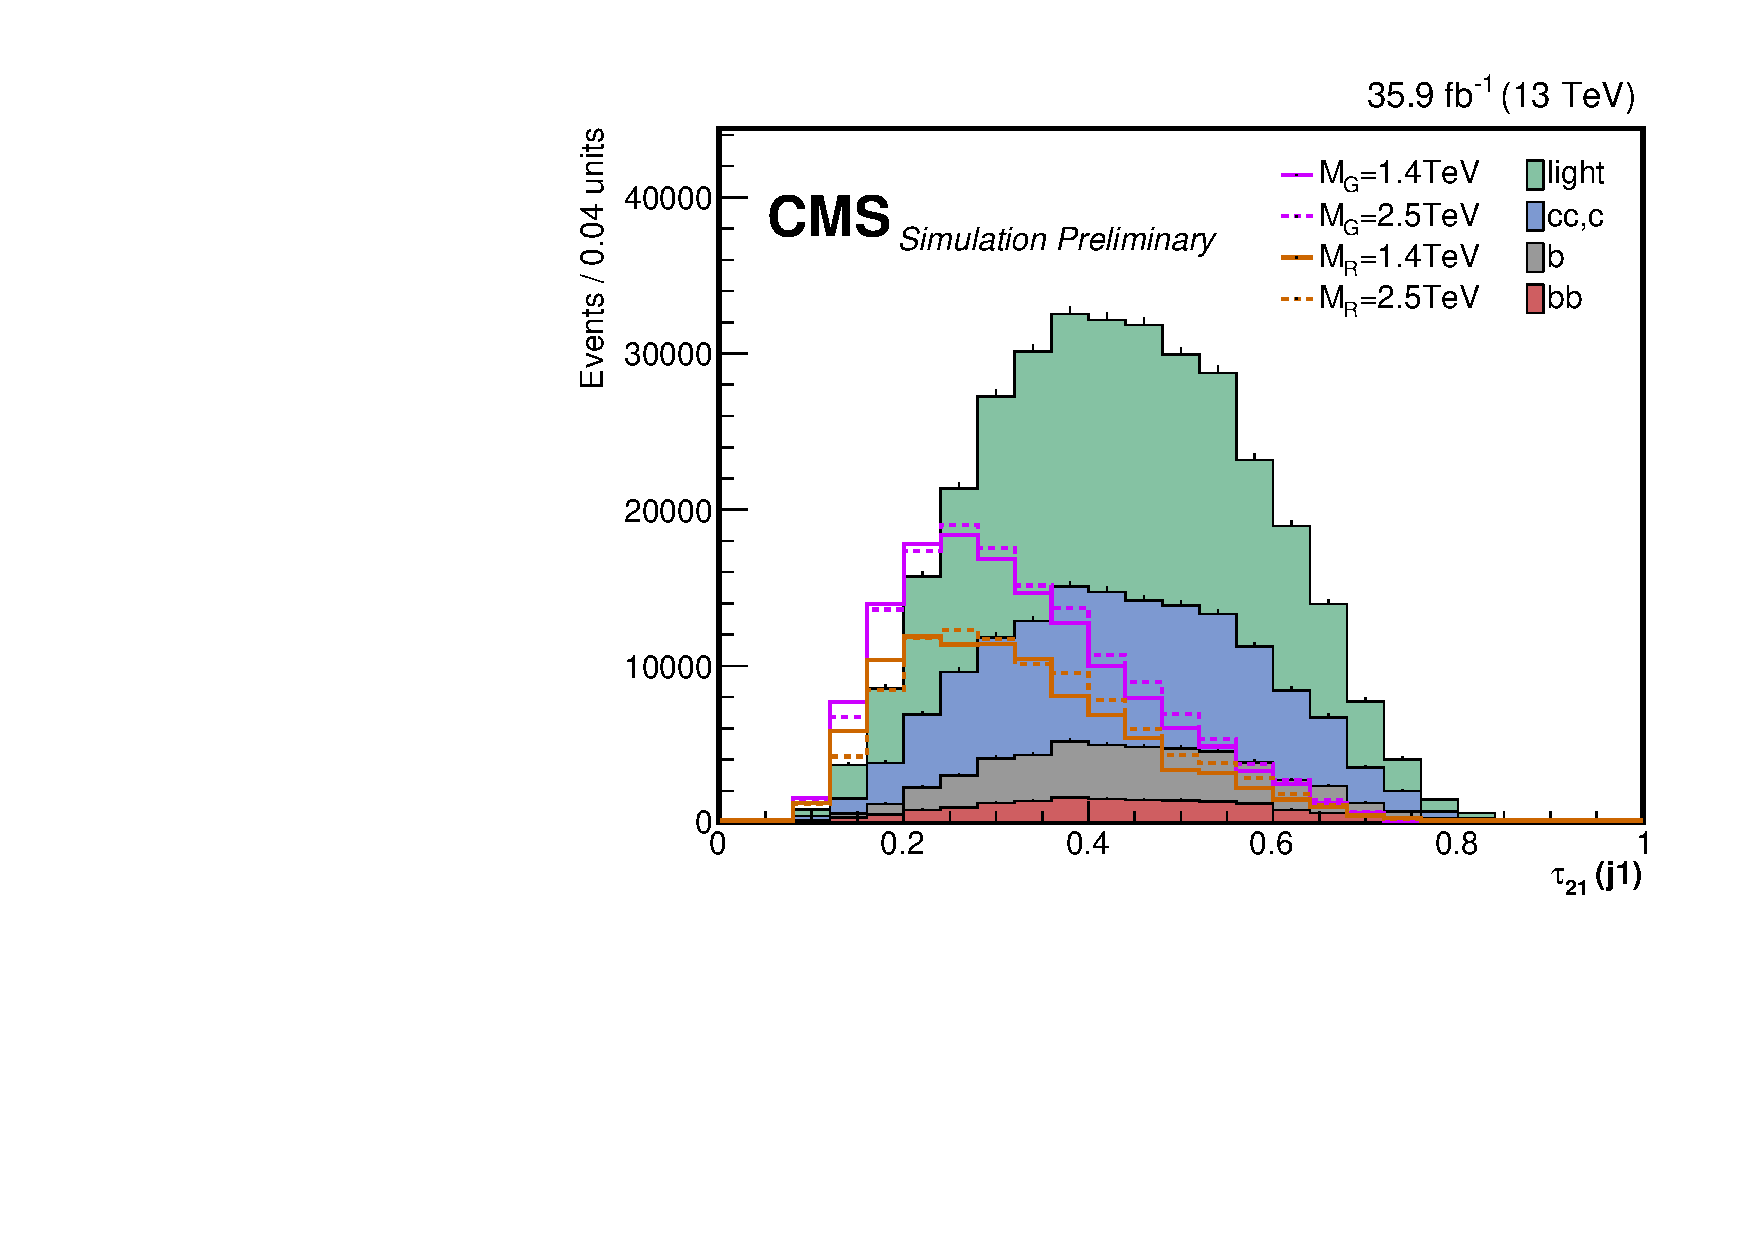
\includegraphics[width=0.5\textwidth]{Figures/MC_N1/puppiTau21_j0.pdf} &
    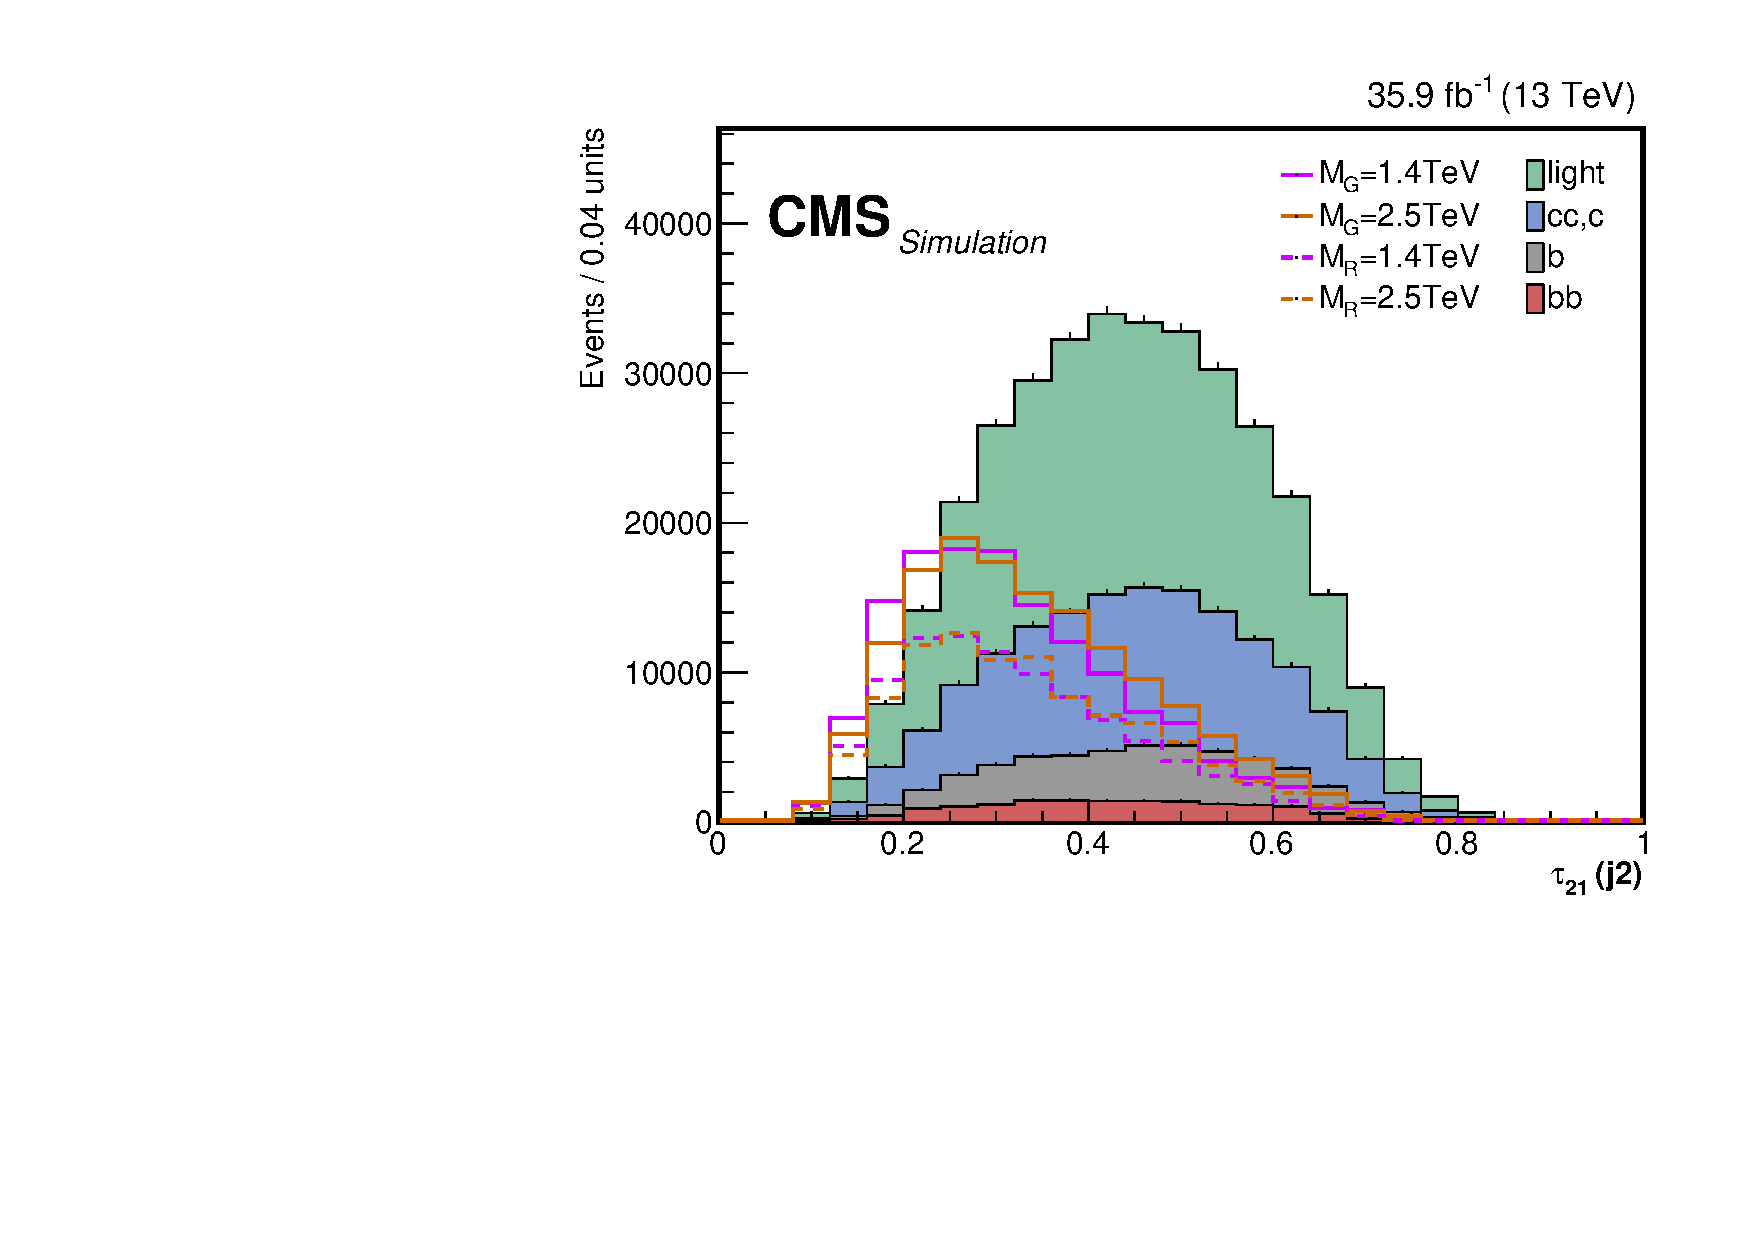
\includegraphics[width=0.5\textwidth]{Figures/MC_N1/puppiTau21_j1.pdf} \\
     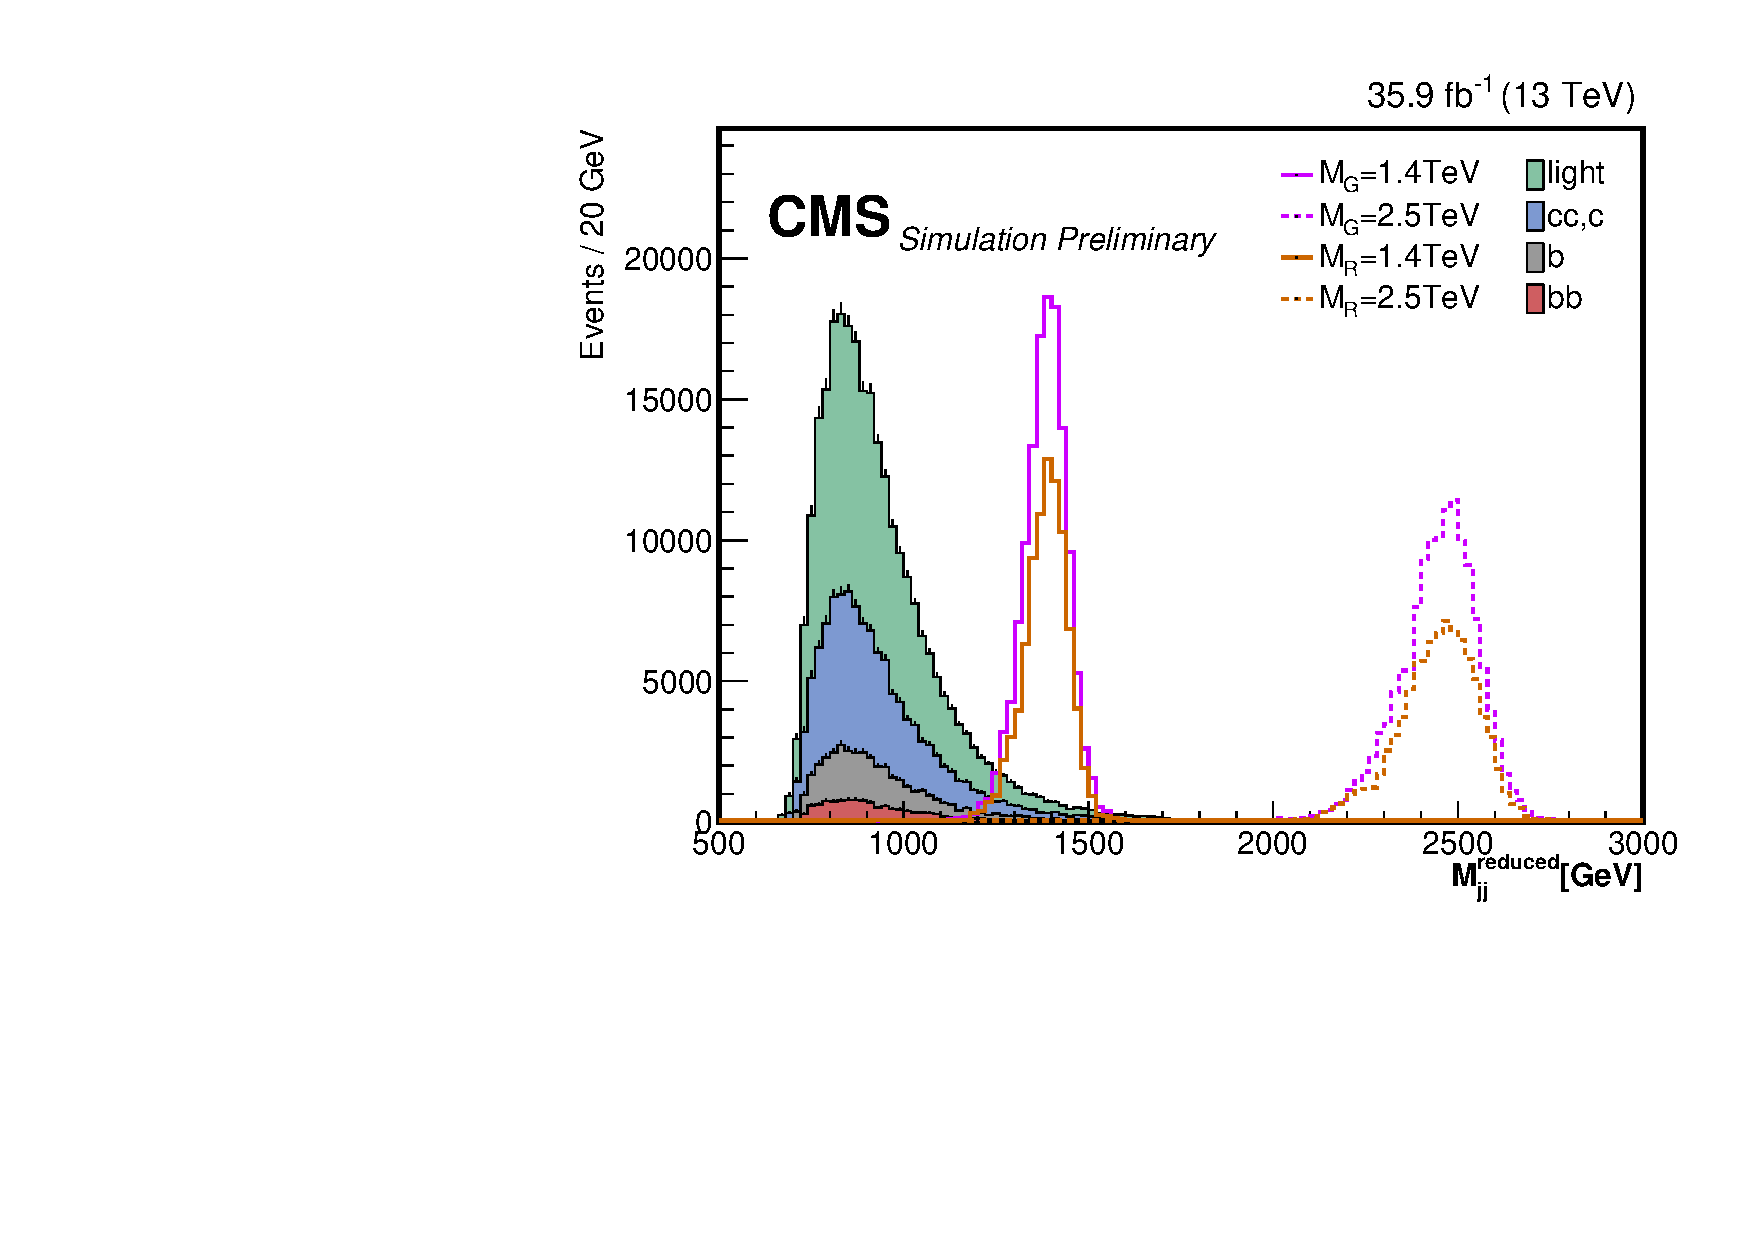
\includegraphics[width=0.5\textwidth]{Figures/MC_N1/totalMassRed.pdf} &
    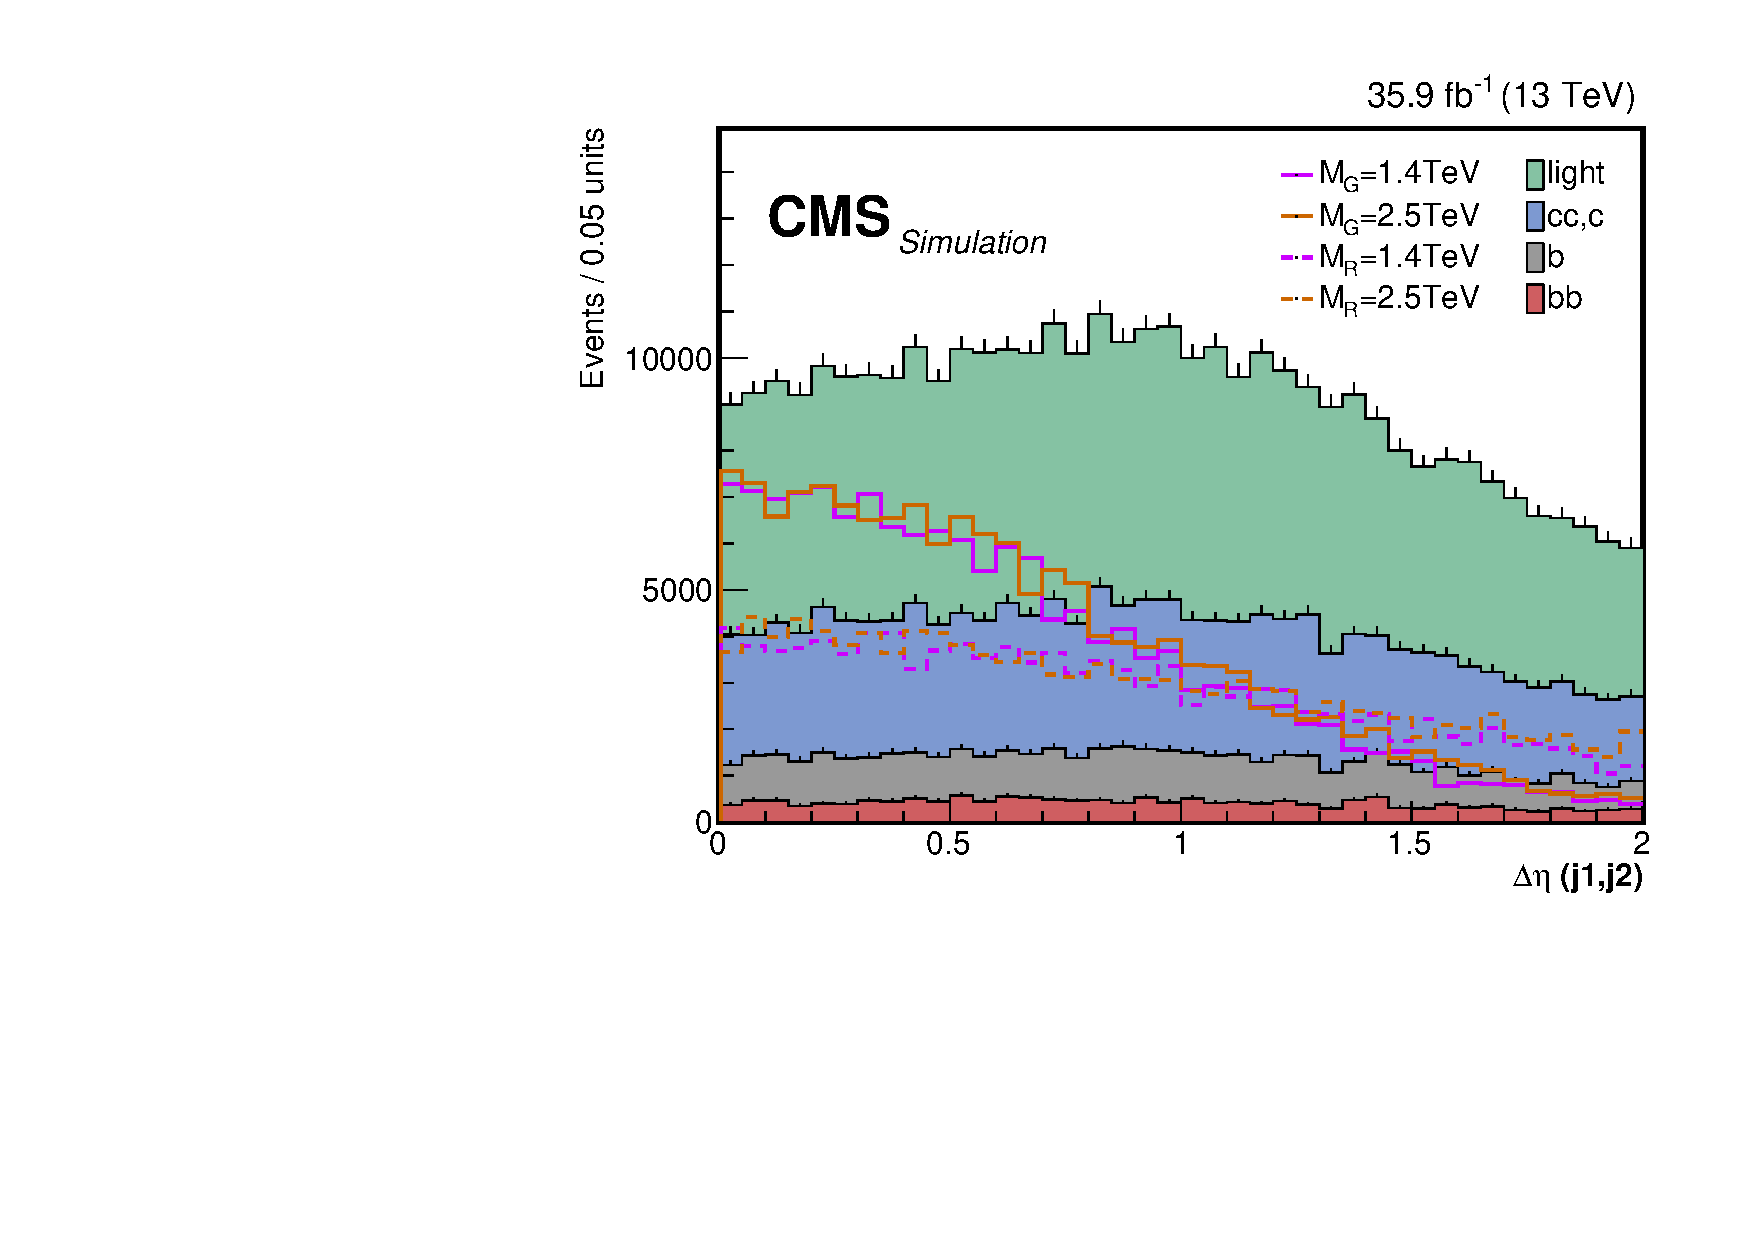
\includegraphics[width=0.5\textwidth]{Figures/MC_N1/deltaEta.pdf} \\
  \end{tabular}
  \caption{The comparison of signal and background. The signals of $M_{X}$ = 1.4 TeV and 2.5 TeV from both models are shown. The cross section is set to 20 pb in the figures. Multi-jet events are seperated into four categories summarized in the table 3.10. From top to buttom are the comparison of PUPPI soft-drop mass, $\tau _{21}$ of leading (left) and next leading (right) AK8 jet, the reduced mass (buttom left), and |$\Delta \eta $ (the two leading AK8 jets)| (buttom right).}
  \label{fig:hvt_brs}
\end{figure}

\section{Data and Monte Carlo Comparison} 
In the section, the comparison of Monte Carlo simulations of background and data will be shown to demonstrate the domiant components in data. Multi-jet events are added up by samples of different $H_T$ section listed in table 3.4, and seperated into four categories summarized in the table 3.10. Besides, the cross sections at leading order of multi-jet events are multiplied by a factor about 0.7 to modify them closer to the value of next leading order.


\begin{itemize}
\item Pile-up re-weighting: all selection is used except $\tau _{21}$ and double-b tagger. The weighting procedure is described in chapter 2.2.
\item Inverse double-b region : all selection is used except only one of double-b taggers passing the loose criteria.
\item Inverse $\tau _{21}$ region: all selection is used except only one of $\tau _{21}$ passing the criteria of 0.55.
\end{itemize} 

\begin{figure}[t]
  \centering
  \begin{tabular}{cc}
    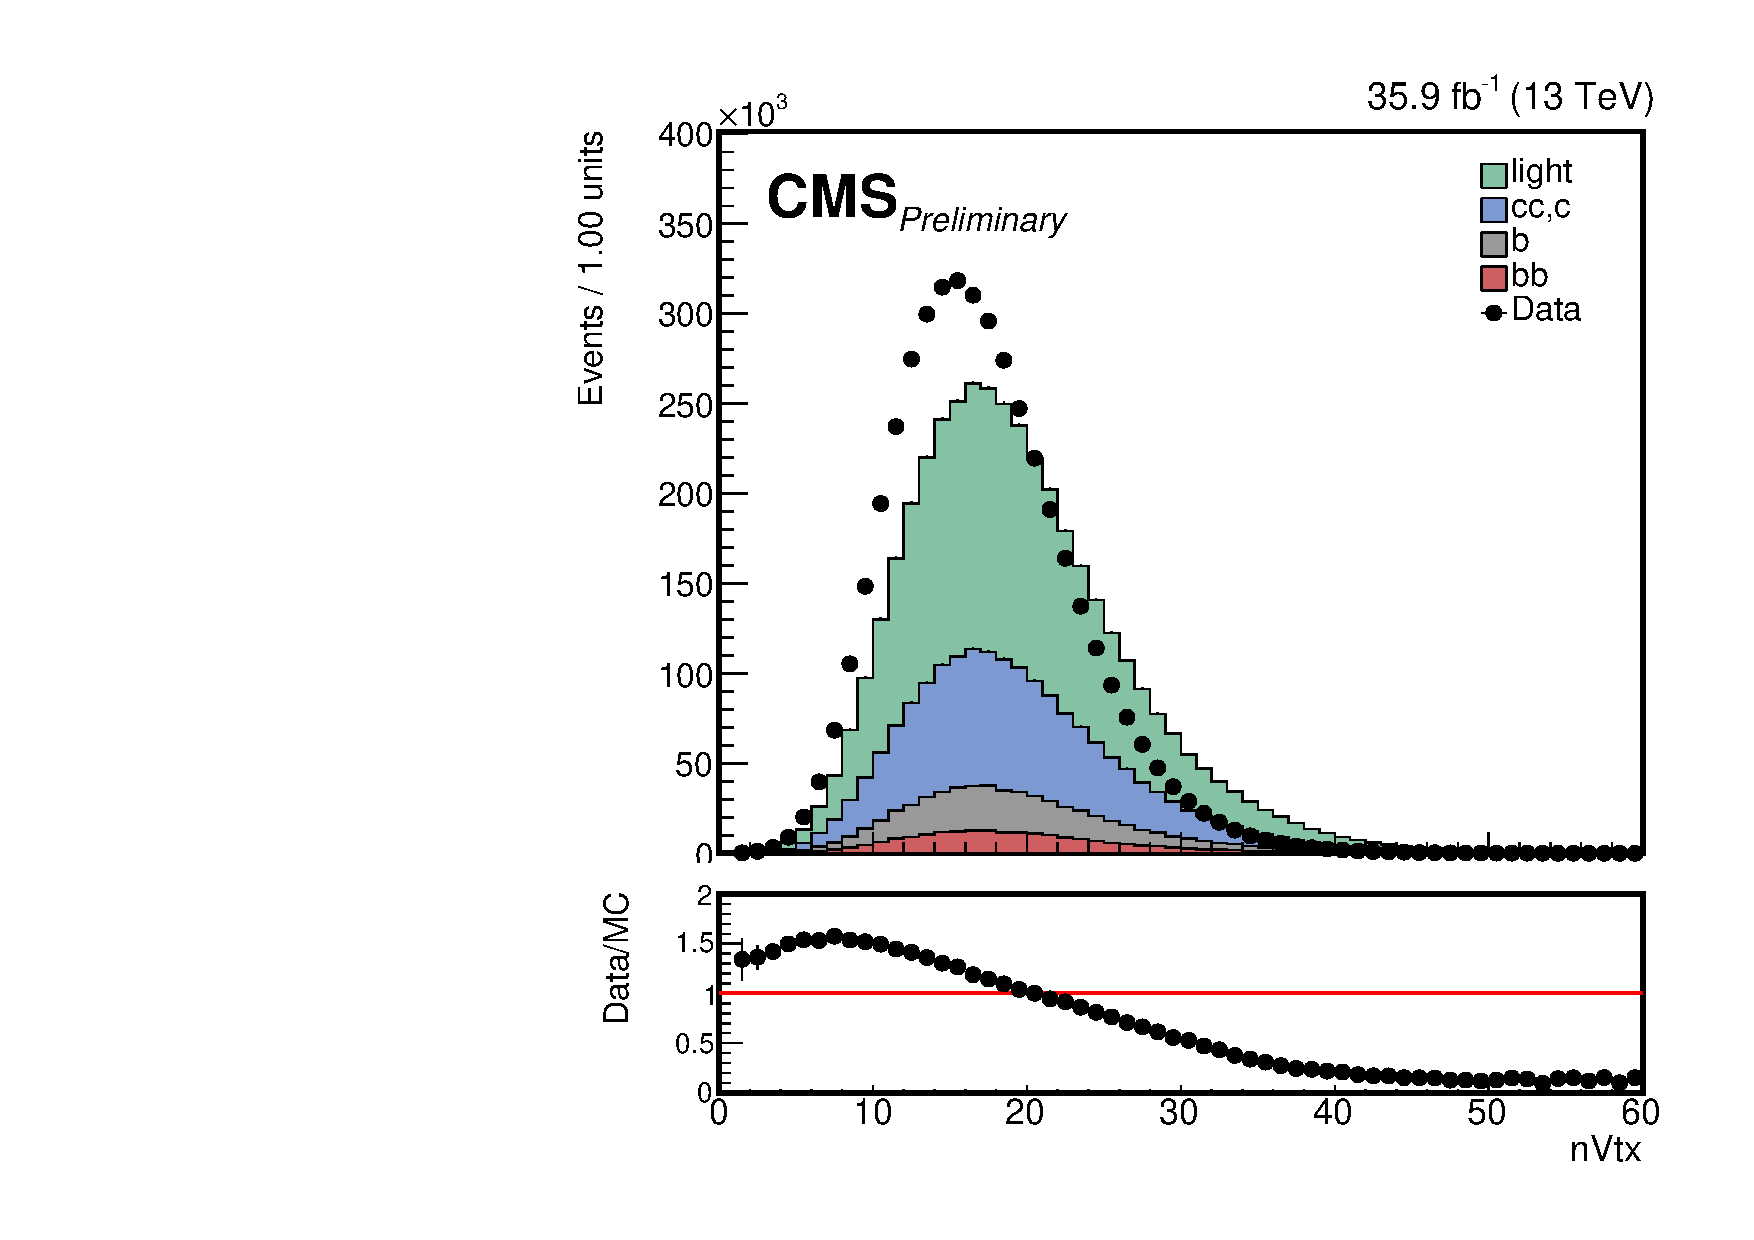
\includegraphics[width=0.5\textwidth]{Figures/dataMC_trig/nVtx.pdf} &
    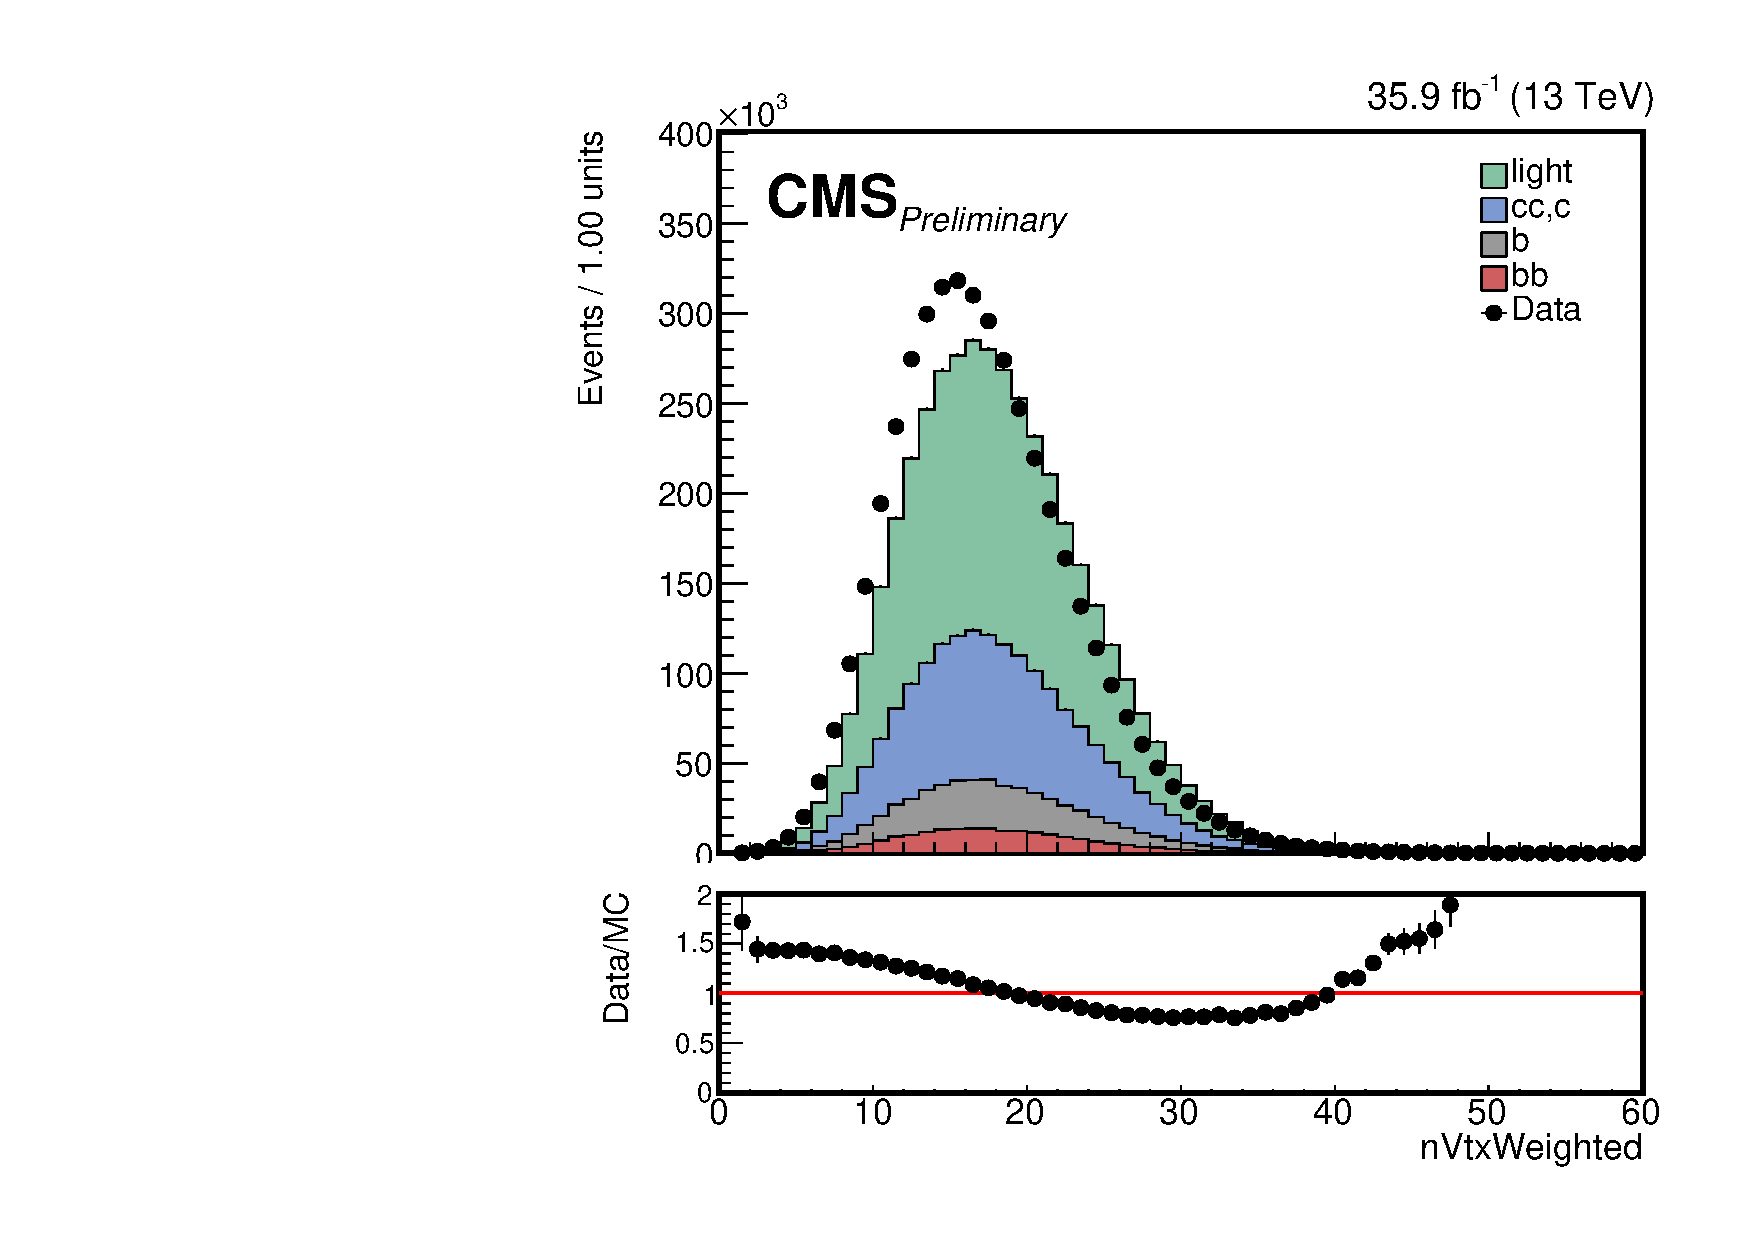
\includegraphics[width=0.5\textwidth]{Figures/dataMC_trig/nVtxWeighted.pdf} \\
    
  \end{tabular}
  \caption{The comparison of data and background of pile-up distribution with (left) and without (right) pile-up re-weighting. Multi-jet events are seperated into four categories summarized in the table 3.10.}
\end{figure}
\begin{figure}[t]
  \centering
  \begin{tabular}{cc}
    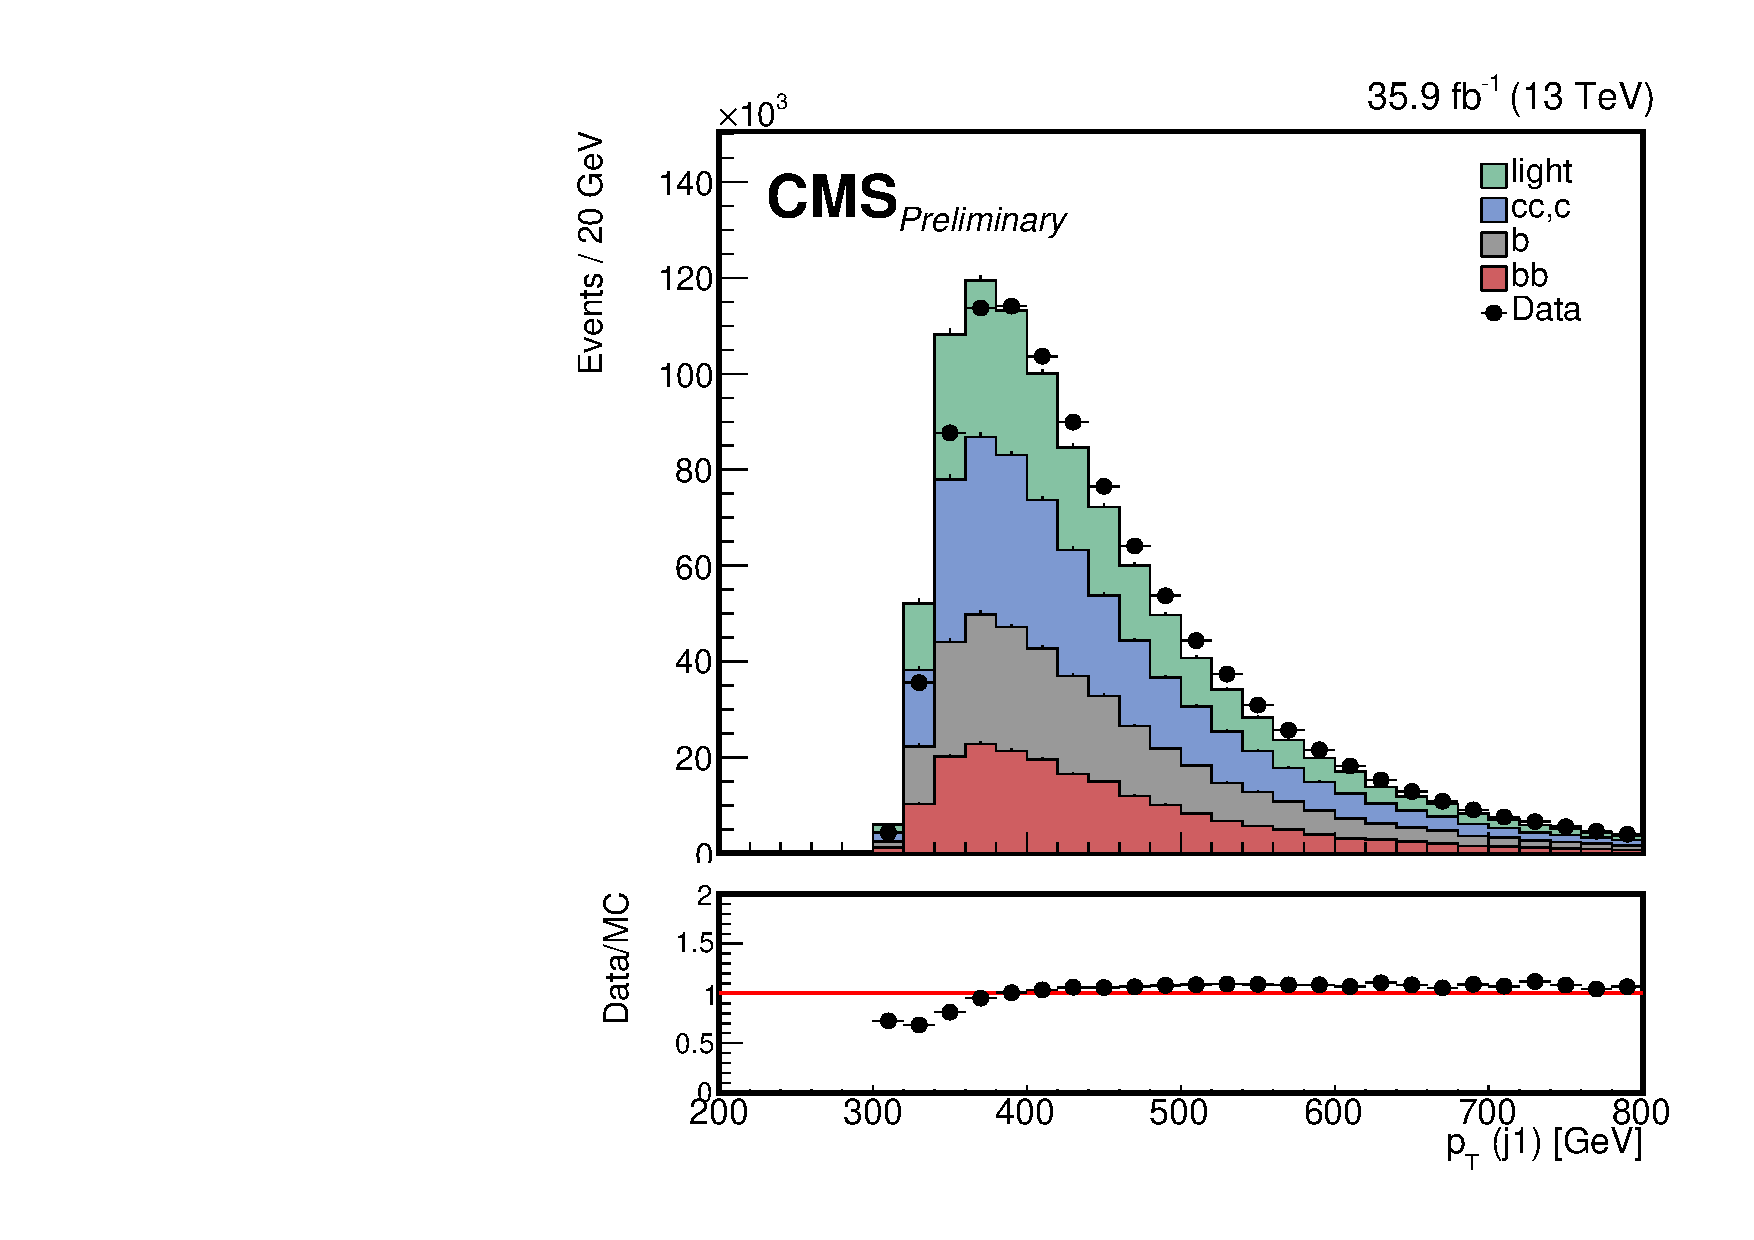
\includegraphics[width=0.5\textwidth]{Figures/dataMC_trig_antiDBT/pt_j0.pdf} &
    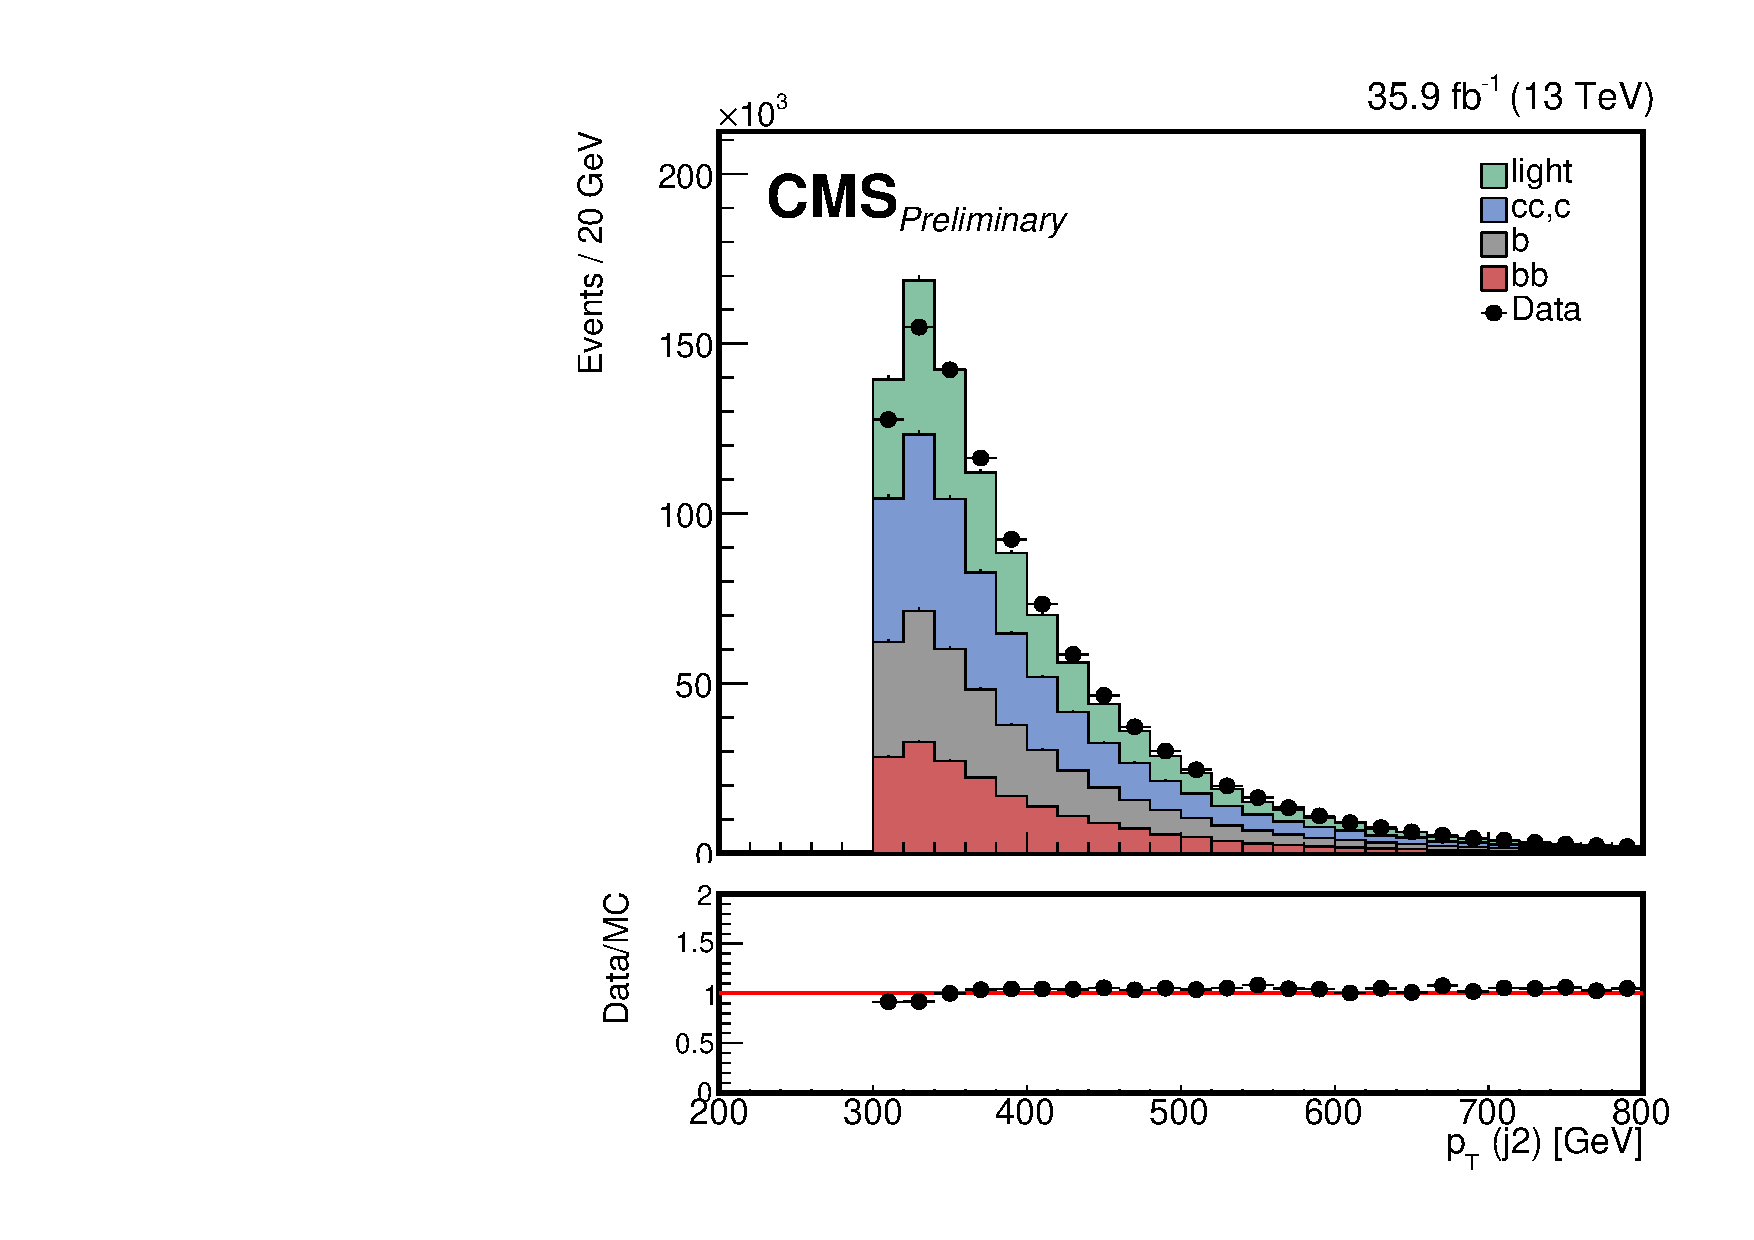
\includegraphics[width=0.5\textwidth]{Figures/dataMC_trig_antiDBT/pt_j1.pdf} \\
     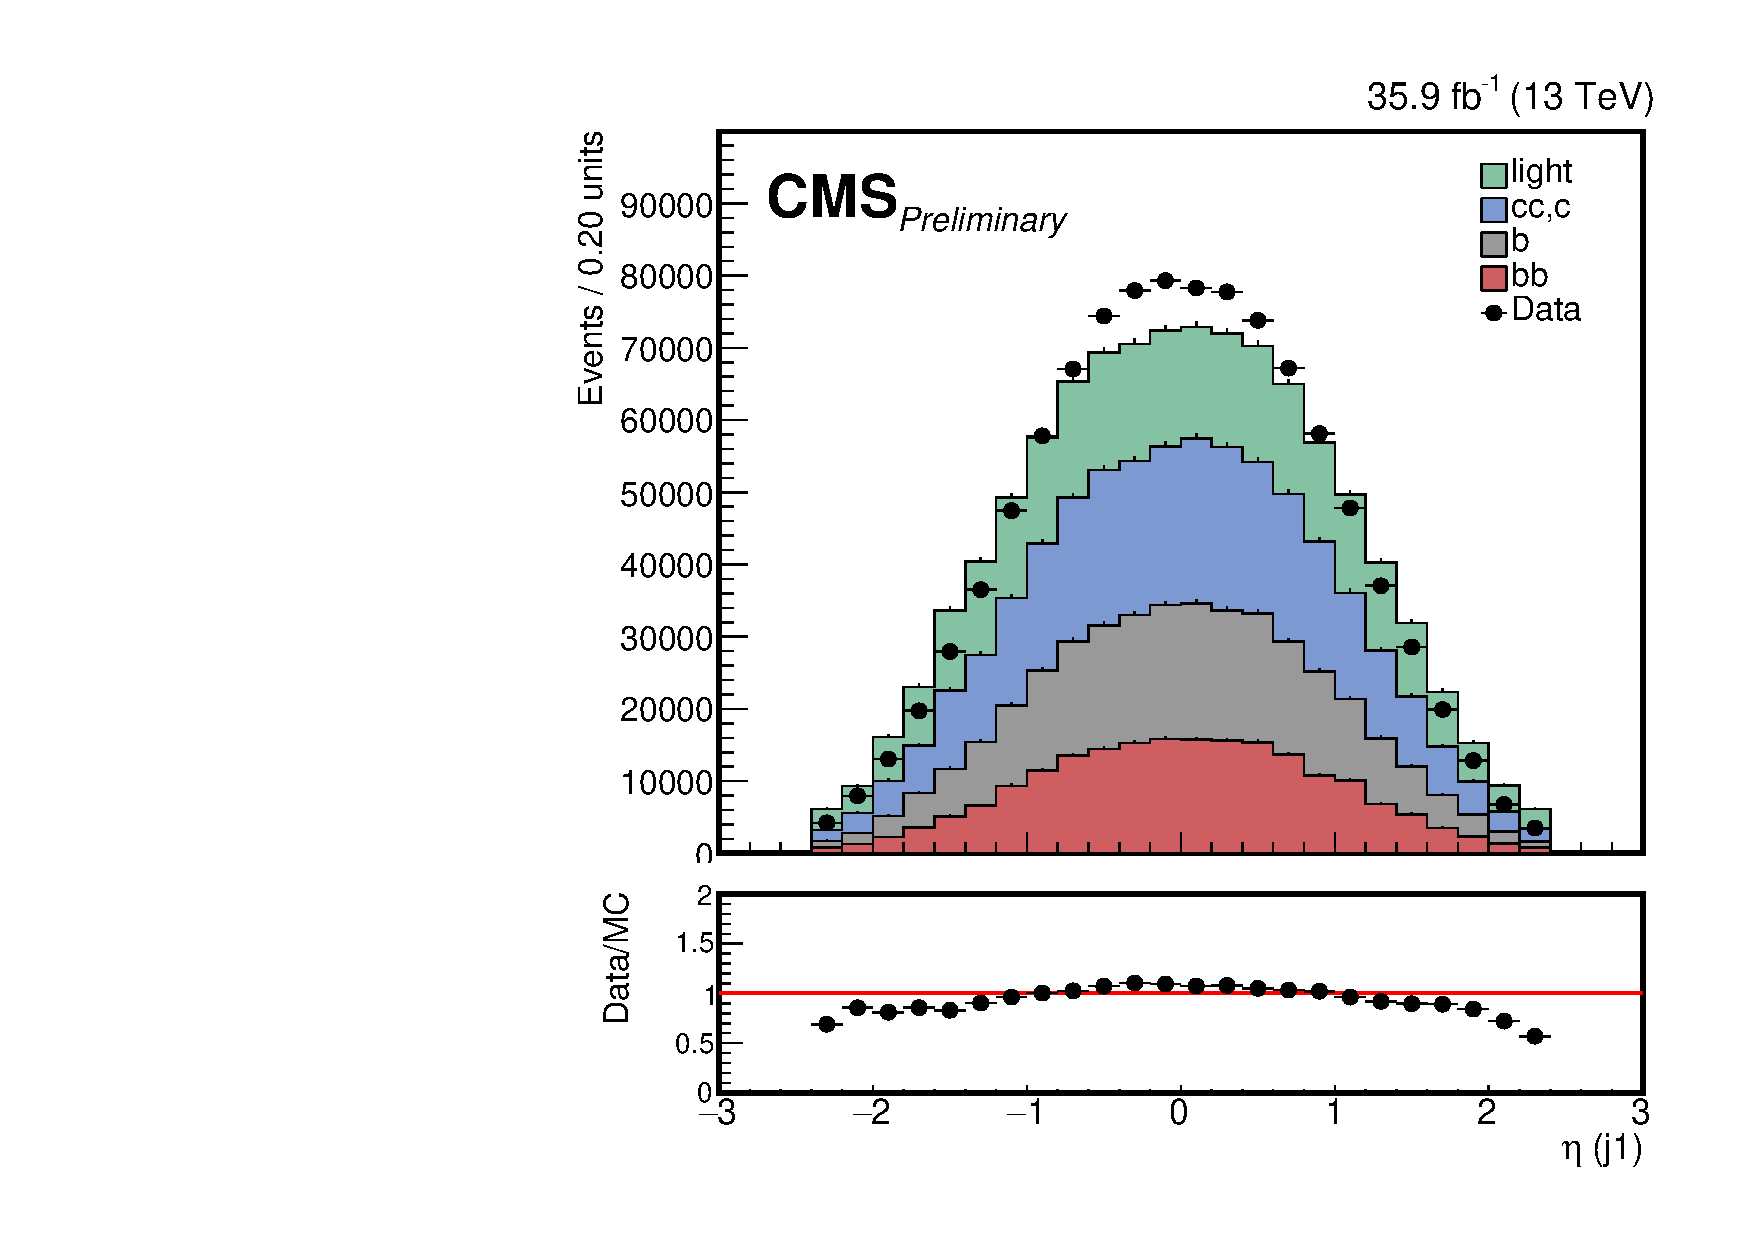
\includegraphics[width=0.5\textwidth]{Figures/dataMC_trig_antiDBT/eta_j0.pdf} &
    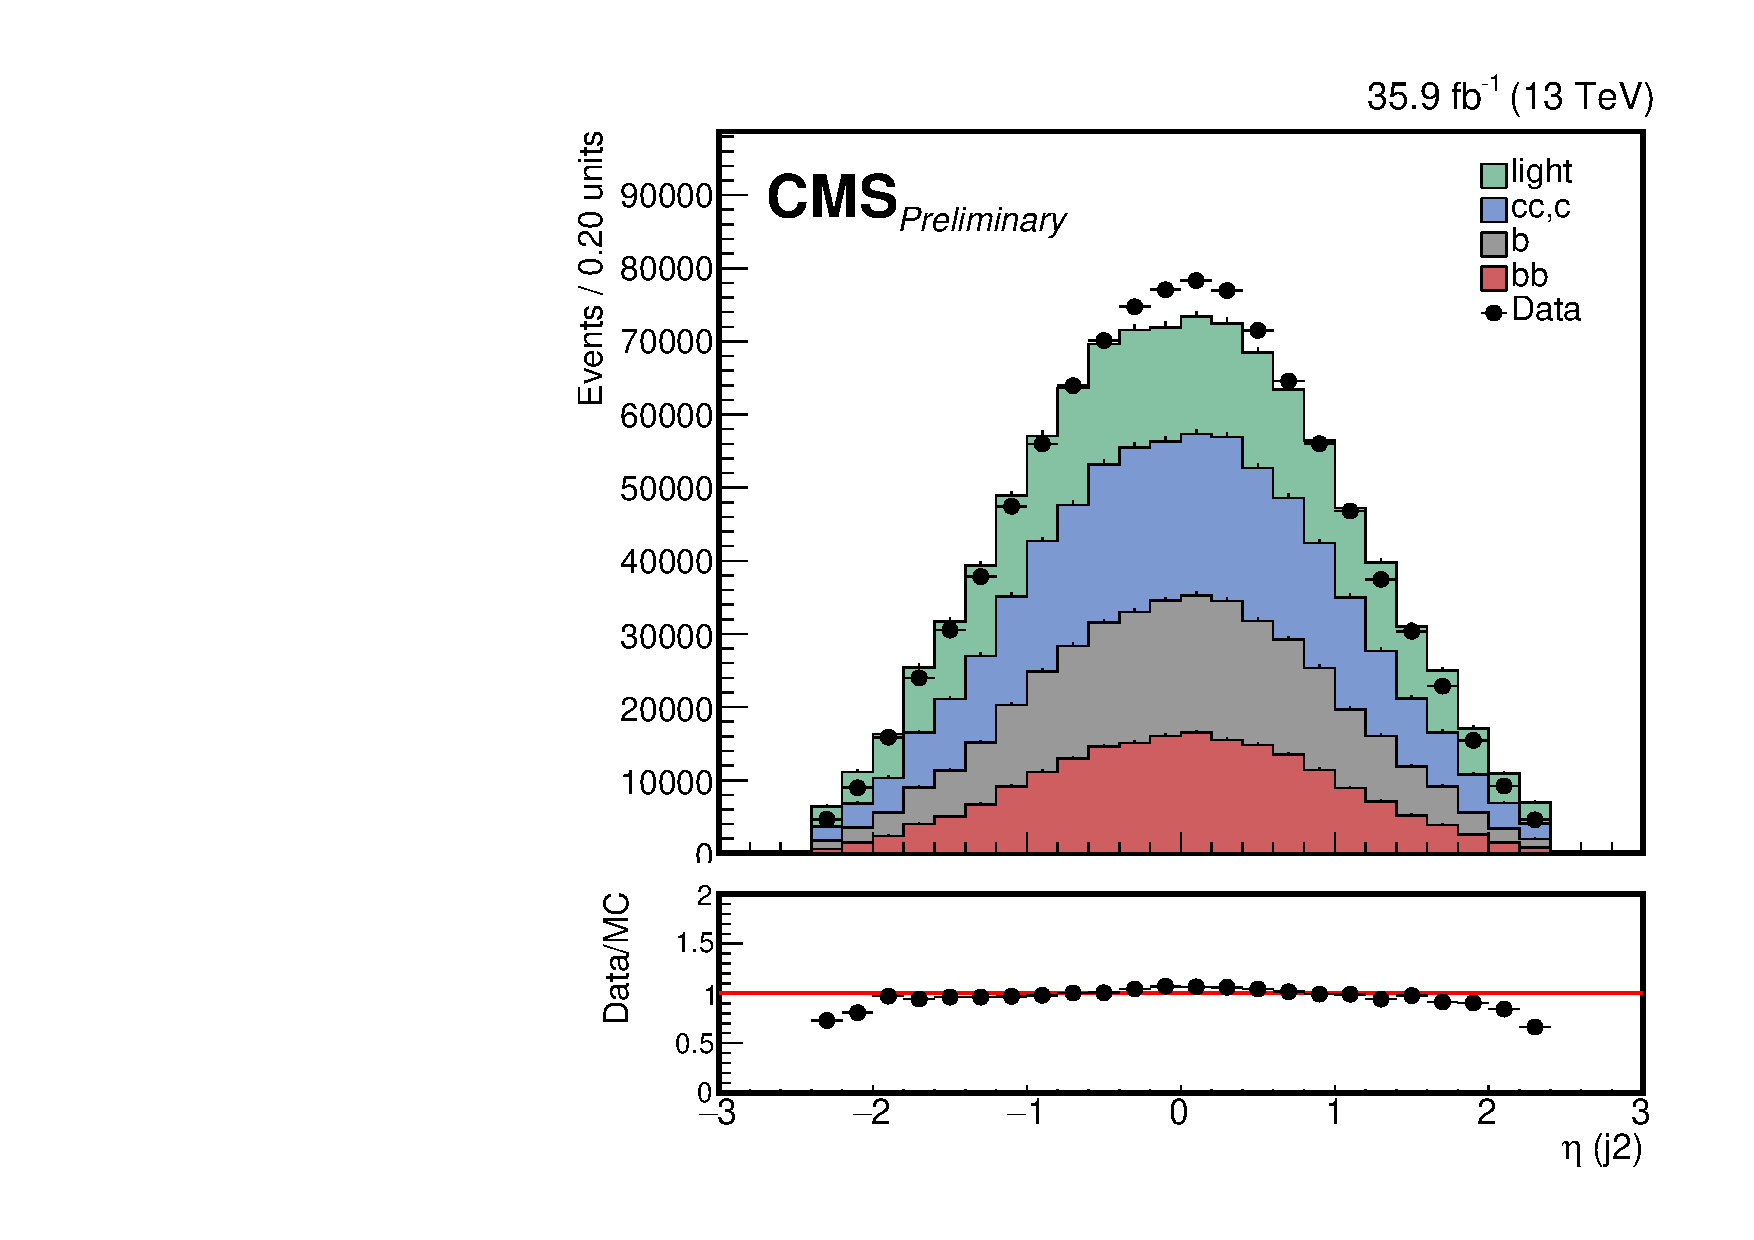
\includegraphics[width=0.5\textwidth]{Figures/dataMC_trig_antiDBT/eta_j1.pdf} \\
     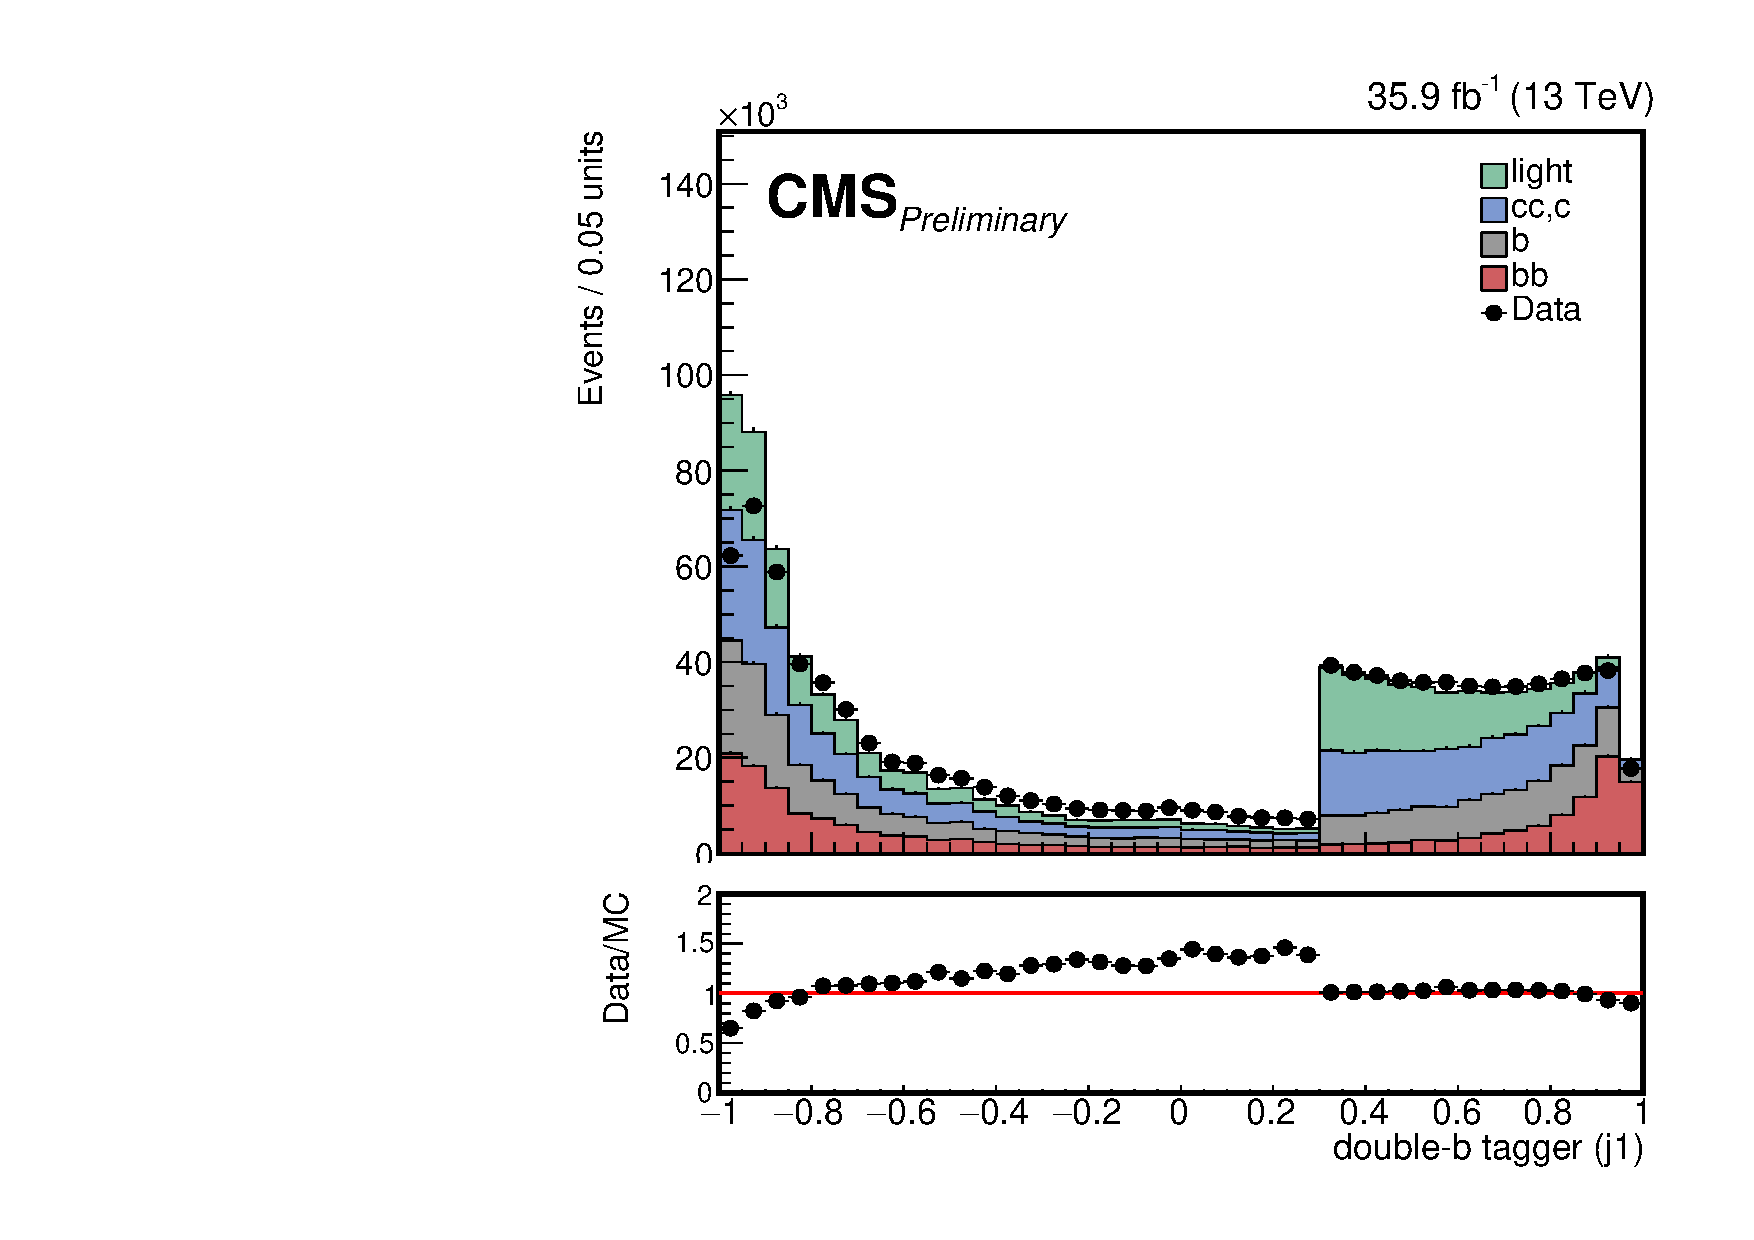
\includegraphics[width=0.5\textwidth]{Figures/dataMC_trig_antiDBT/doubleSV_j0.pdf} &
    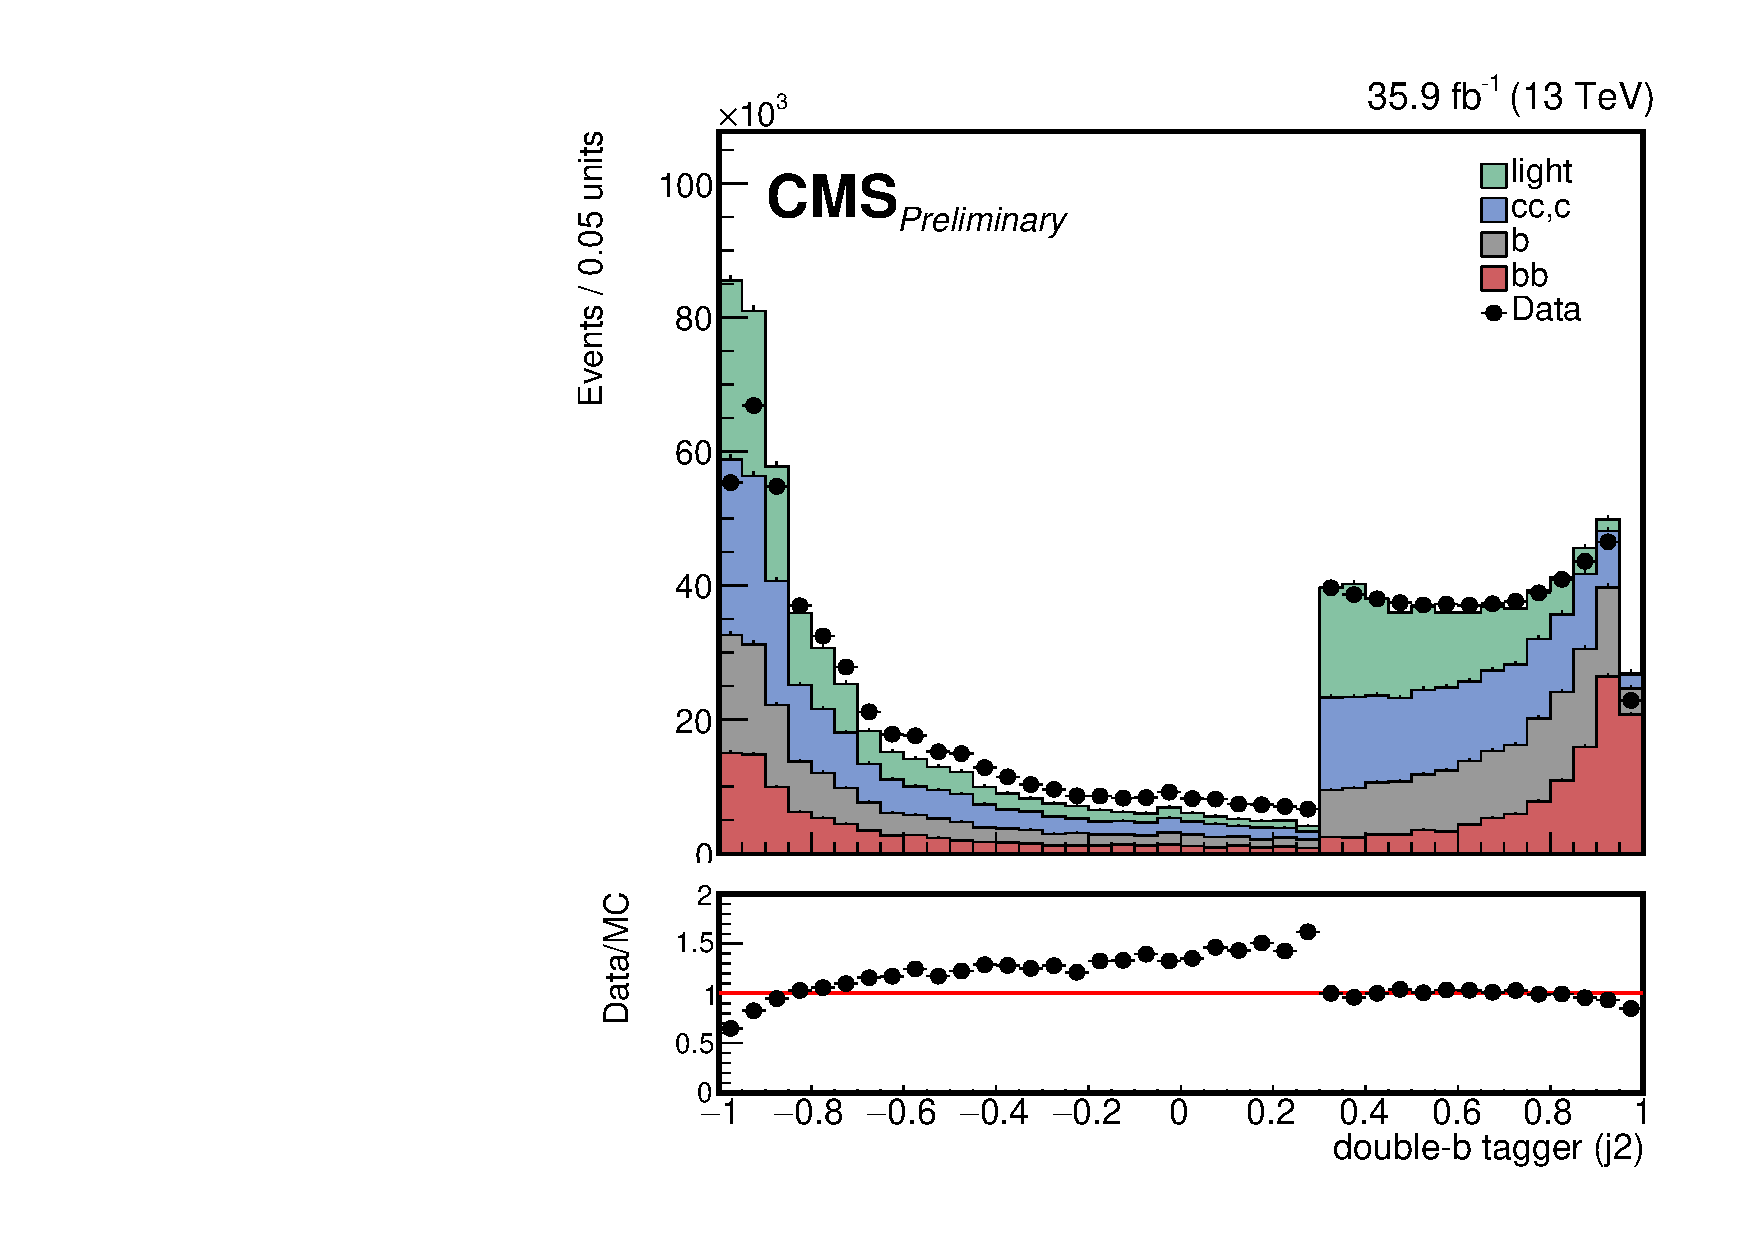
\includegraphics[width=0.5\textwidth]{Figures/dataMC_trig_antiDBT/doubleSV_j1.pdf} \\
  \end{tabular}
  \caption{The comparison of data and background in inverse double-b region. Multi-jet events are seperated into four categories summarized in the table 3.10. From top to buttom are the comparison of $p_{T}$, $\eta $, and double-b tagger of leading (left) and next leading (right) AK8 jet.}
  \label{fig:hvt_brs}
\end{figure}
\begin{figure}[t]
  \centering
  \begin{tabular}{cc}
    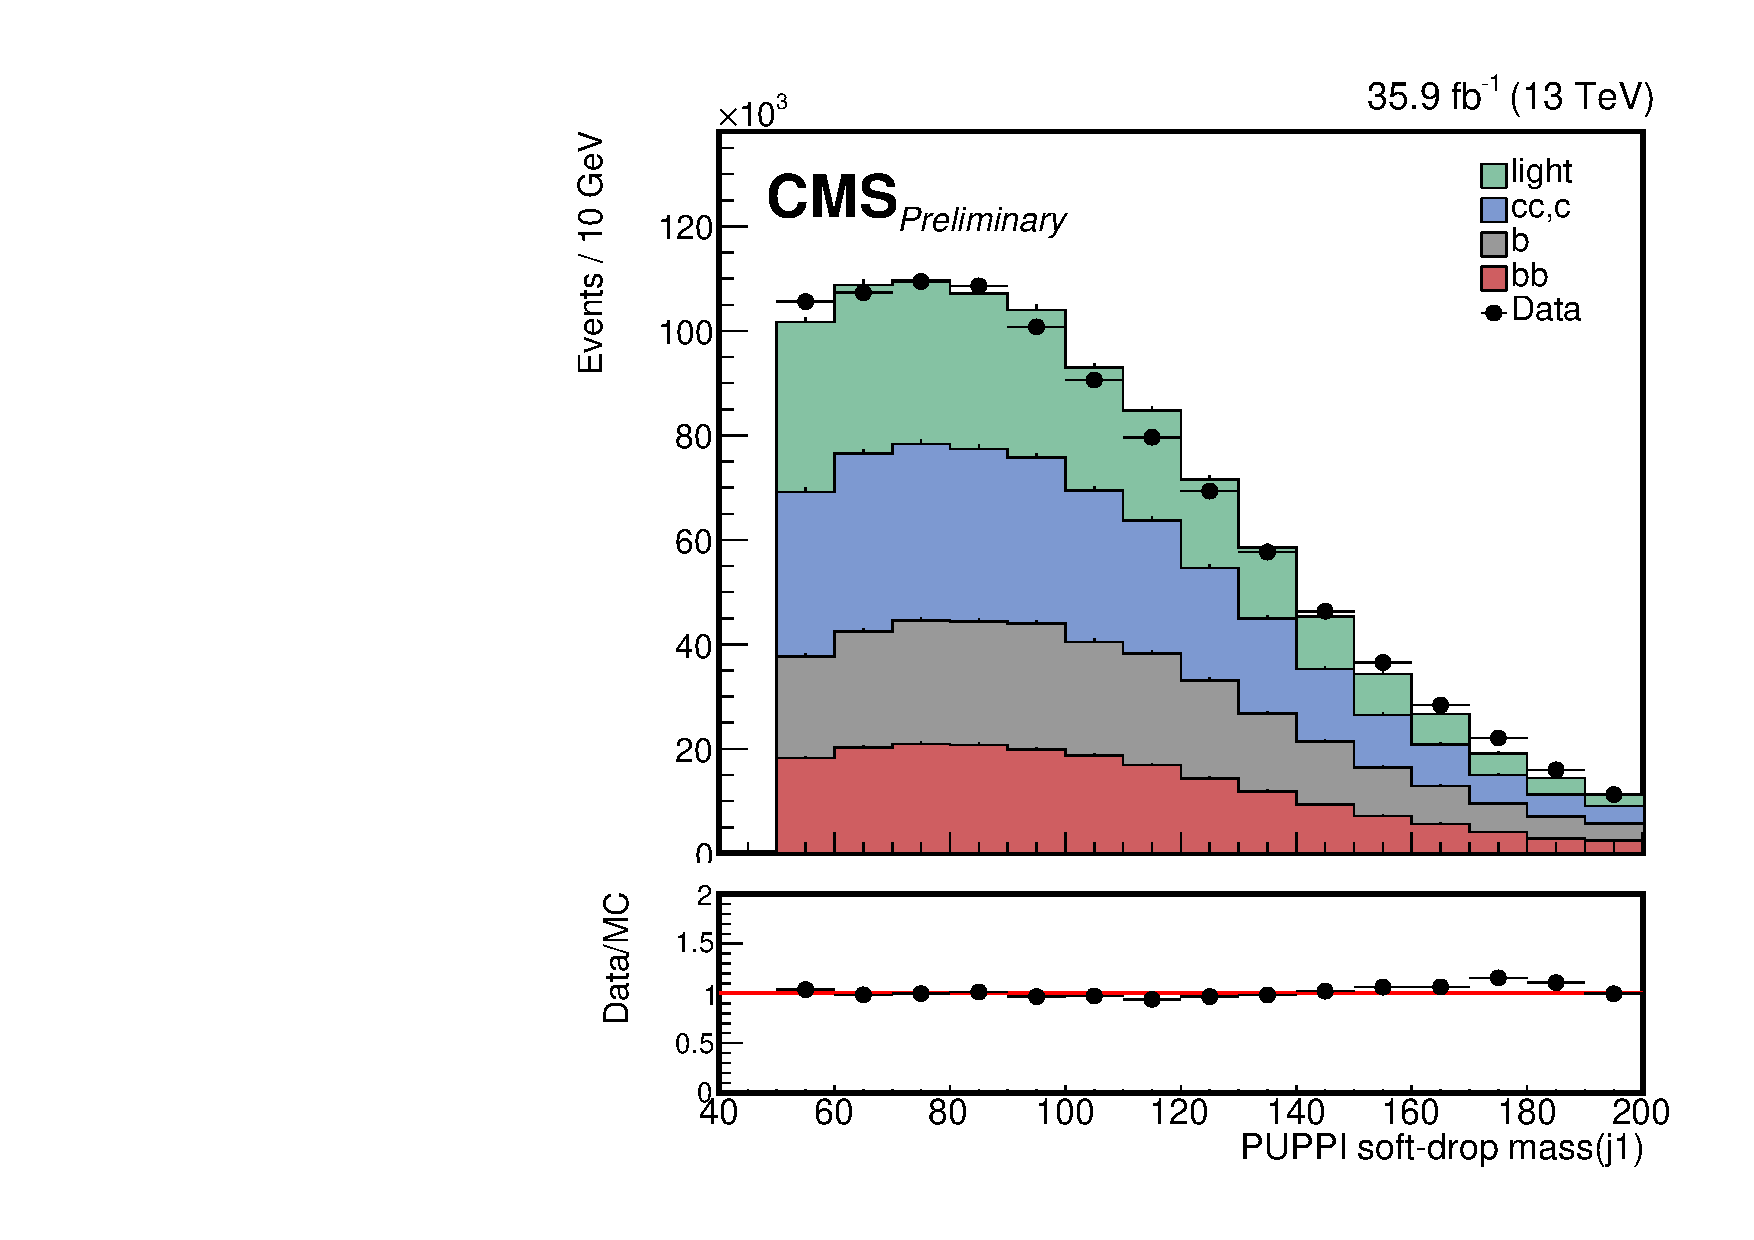
\includegraphics[width=0.5\textwidth]{Figures/dataMC_trig_antiDBT/puppiSDMassThea_j0.pdf} &
    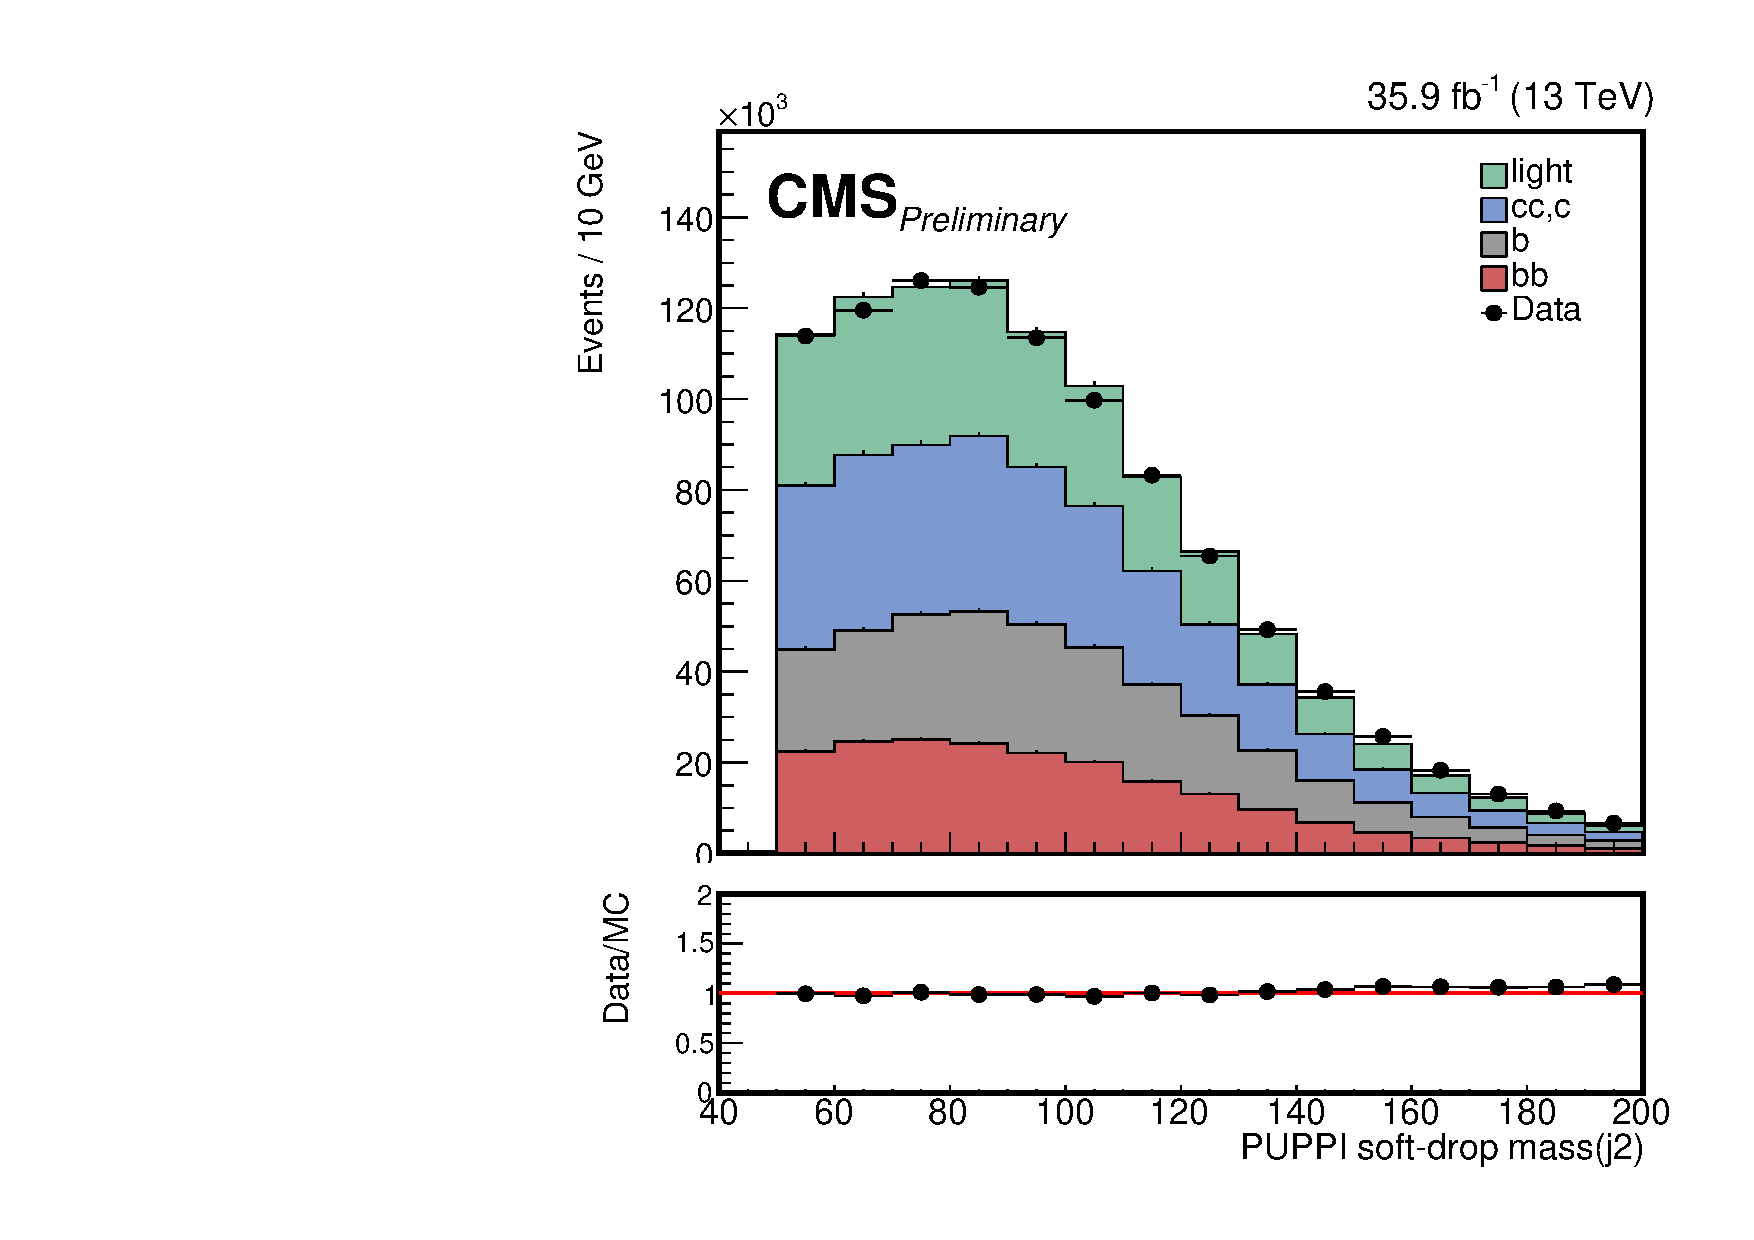
\includegraphics[width=0.5\textwidth]{Figures/dataMC_trig_antiDBT/puppiSDMassThea_j1.pdf} \\
     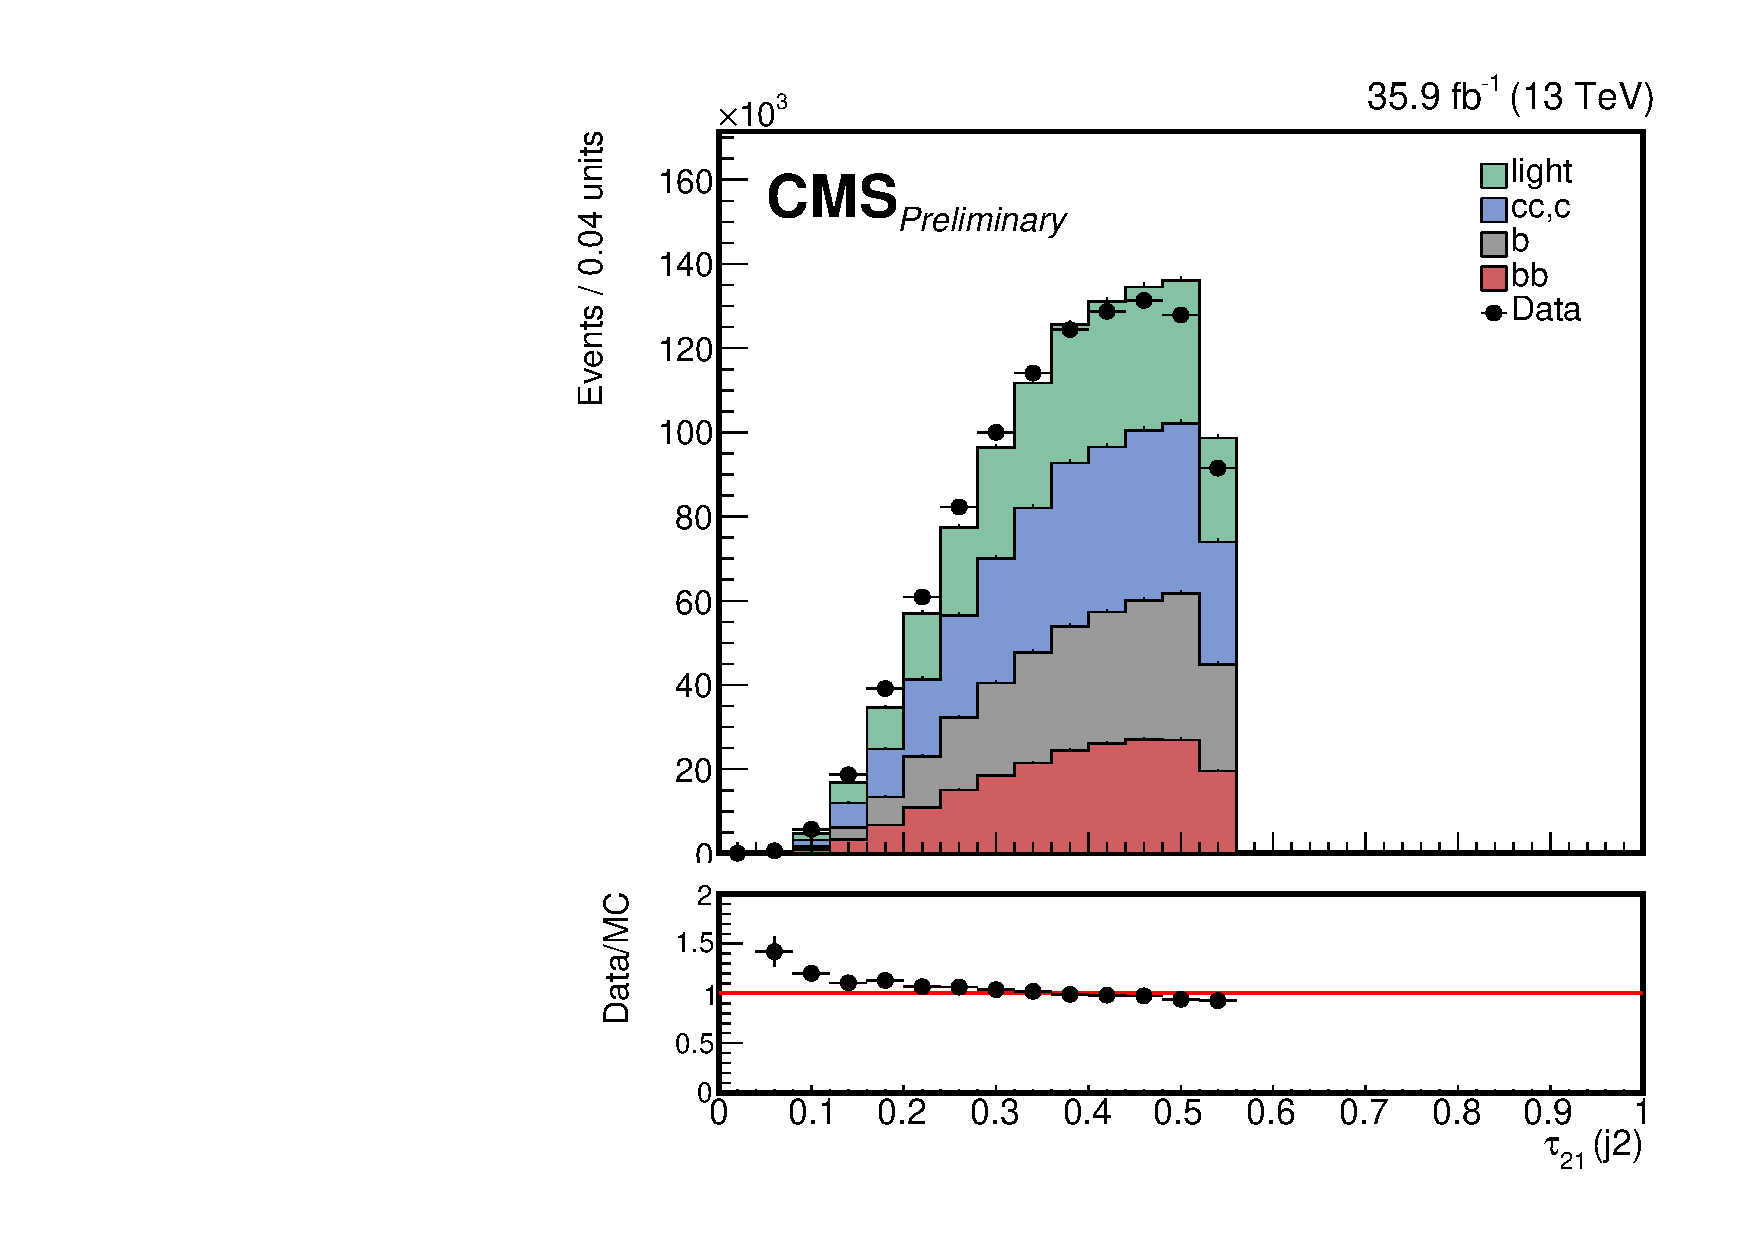
\includegraphics[width=0.5\textwidth]{Figures/dataMC_trig_antiDBT/puppiTau21_j0.pdf} &
    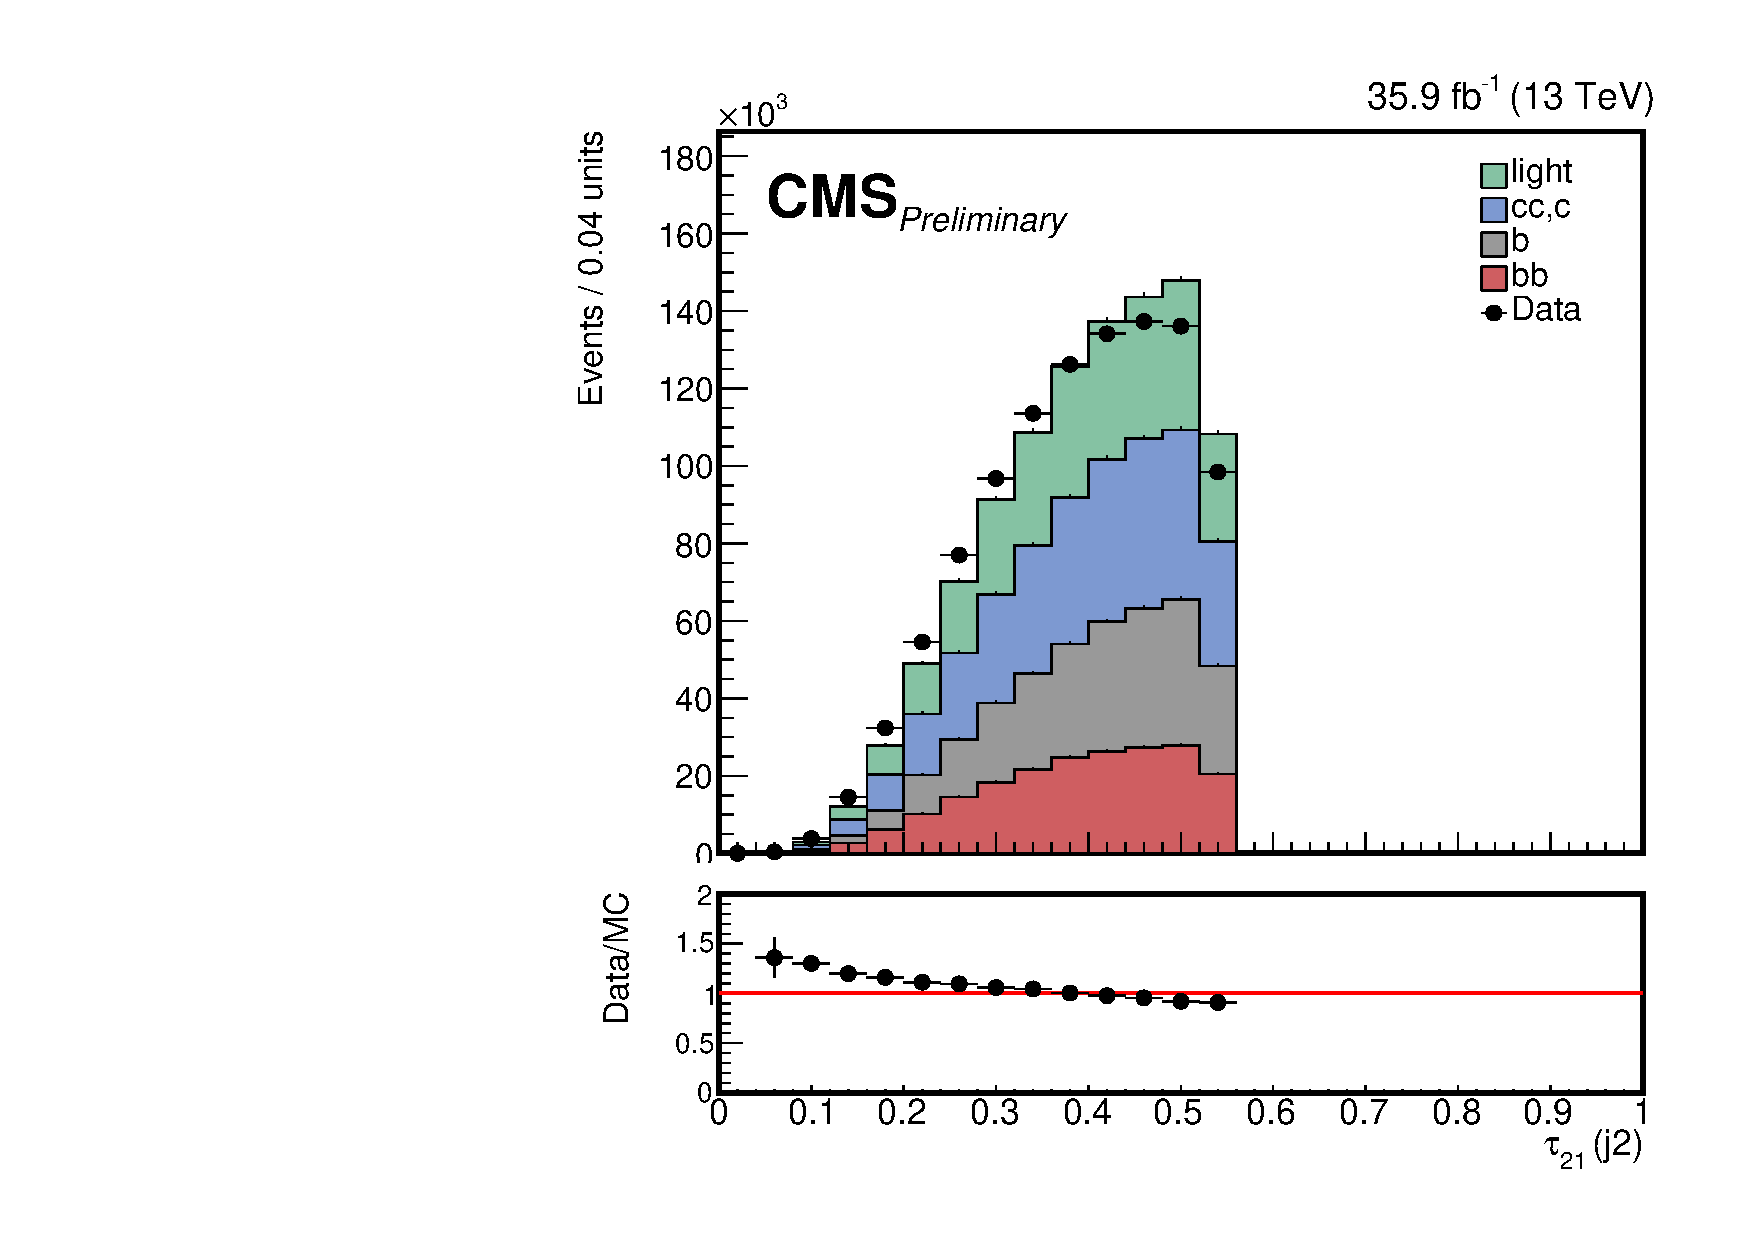
\includegraphics[width=0.5\textwidth]{Figures/dataMC_trig_antiDBT/puppiTau21_j1.pdf} \\
     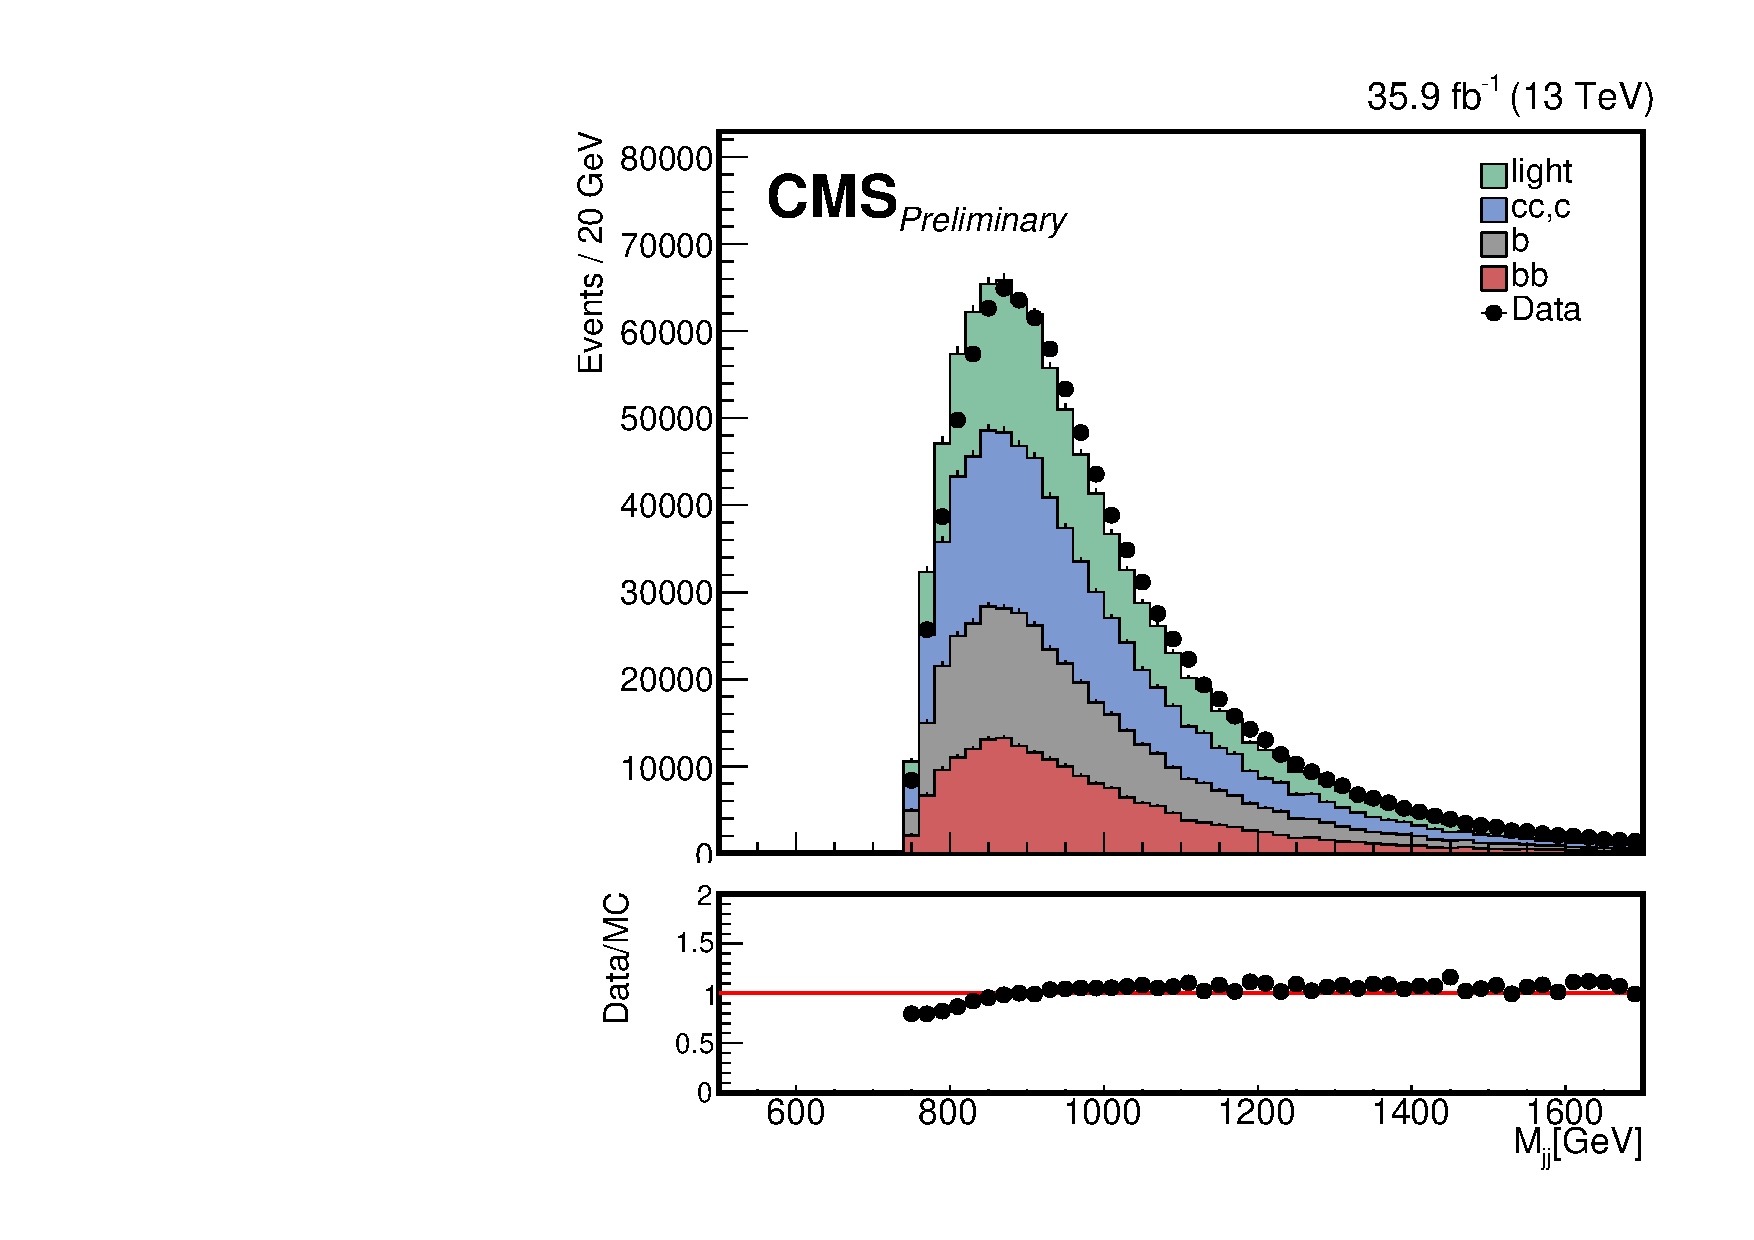
\includegraphics[width=0.5\textwidth]{Figures/dataMC_trig_antiDBT/totalMassRed.pdf} &
    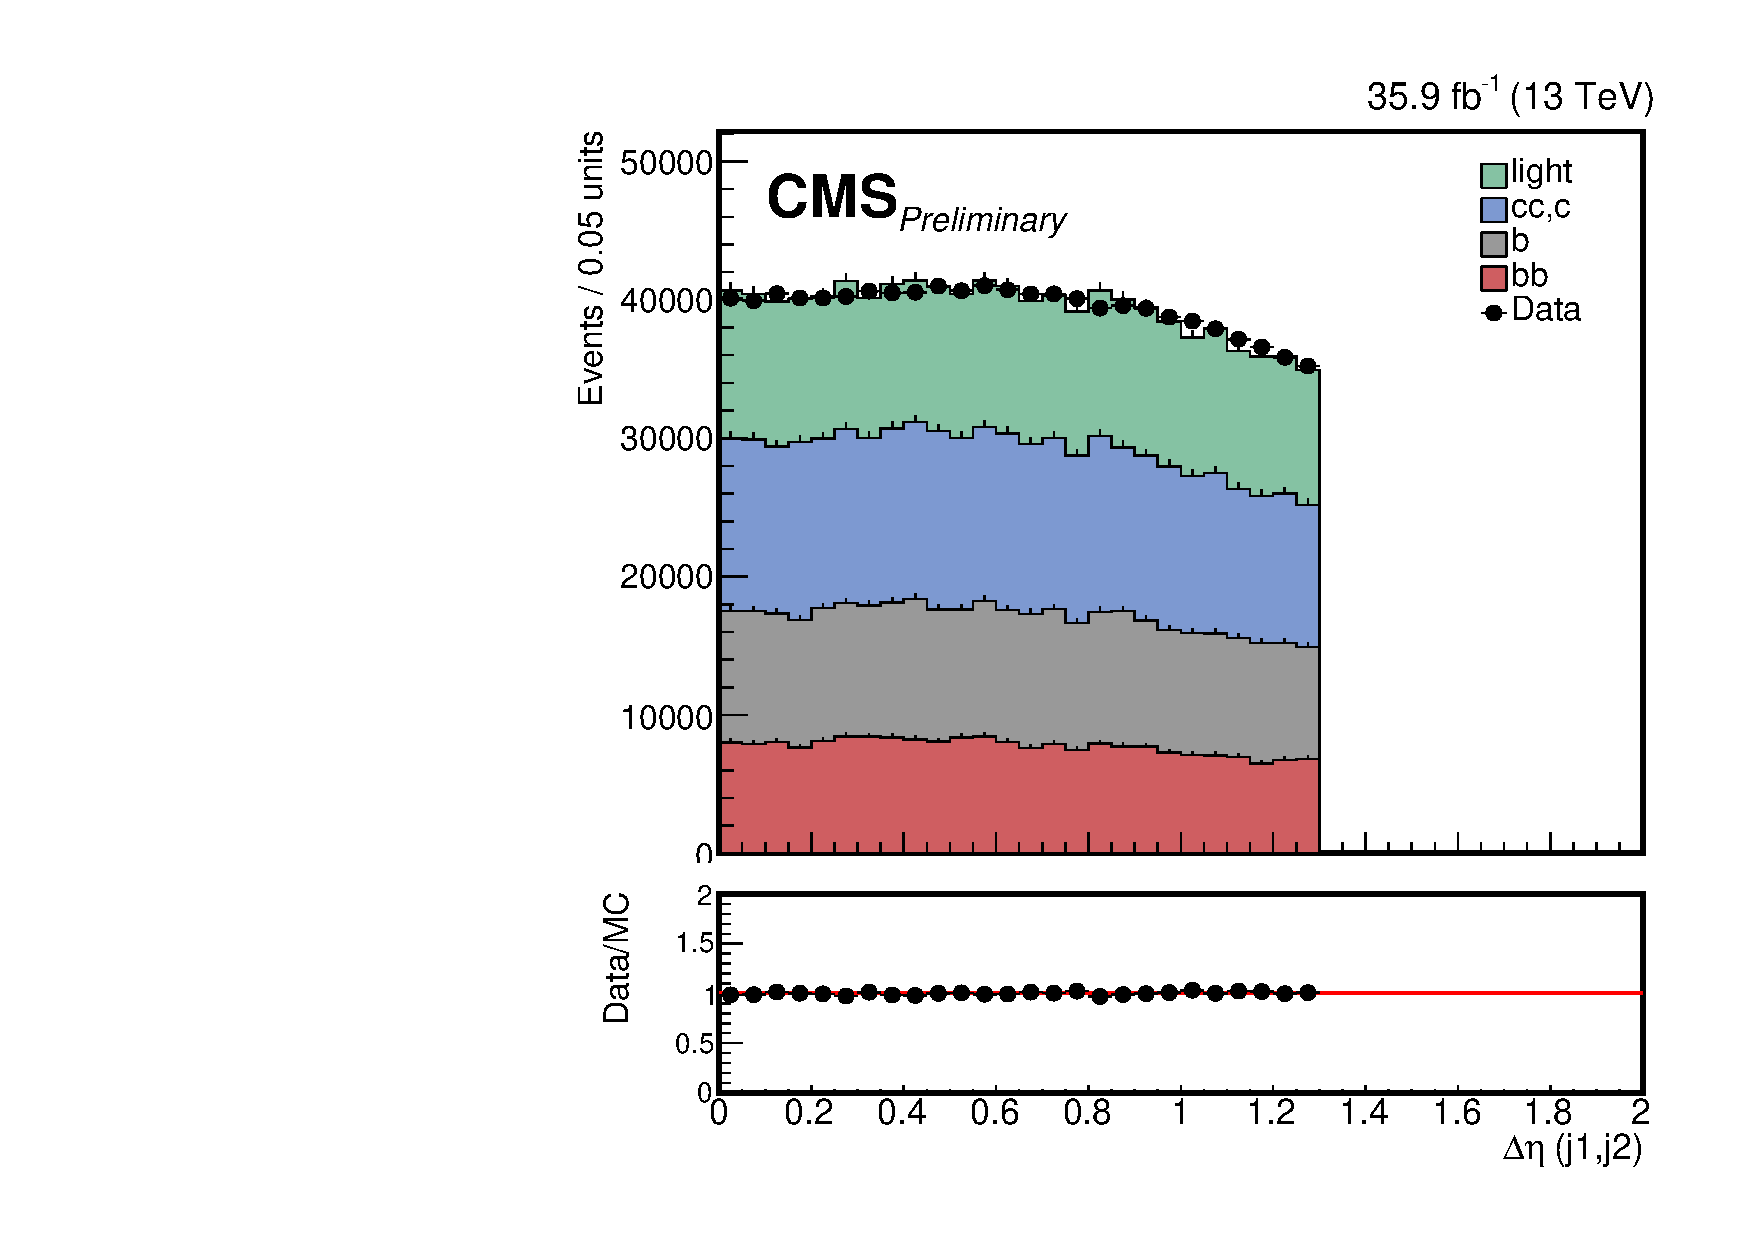
\includegraphics[width=0.5\textwidth]{Figures/dataMC_trig_antiDBT/deltaEta.pdf} \\
  \end{tabular}
  \caption{The comparison of data and background in inverse double-b region. Multi-jet events are seperated into four categories summarized in the table 3.10. From top to buttom are the comparison of PUPPI soft-drop mass, $\tau _{21}$ of leading (left) and next leading (right) AK8 jet, the reduced mass (buttom left), and |$\Delta \eta $ (the two leading AK8 jets)| (buttom right).}
  \label{fig:hvt_brs}
\end{figure}

\begin{figure}[t]
  \centering
  \begin{tabular}{cc}
    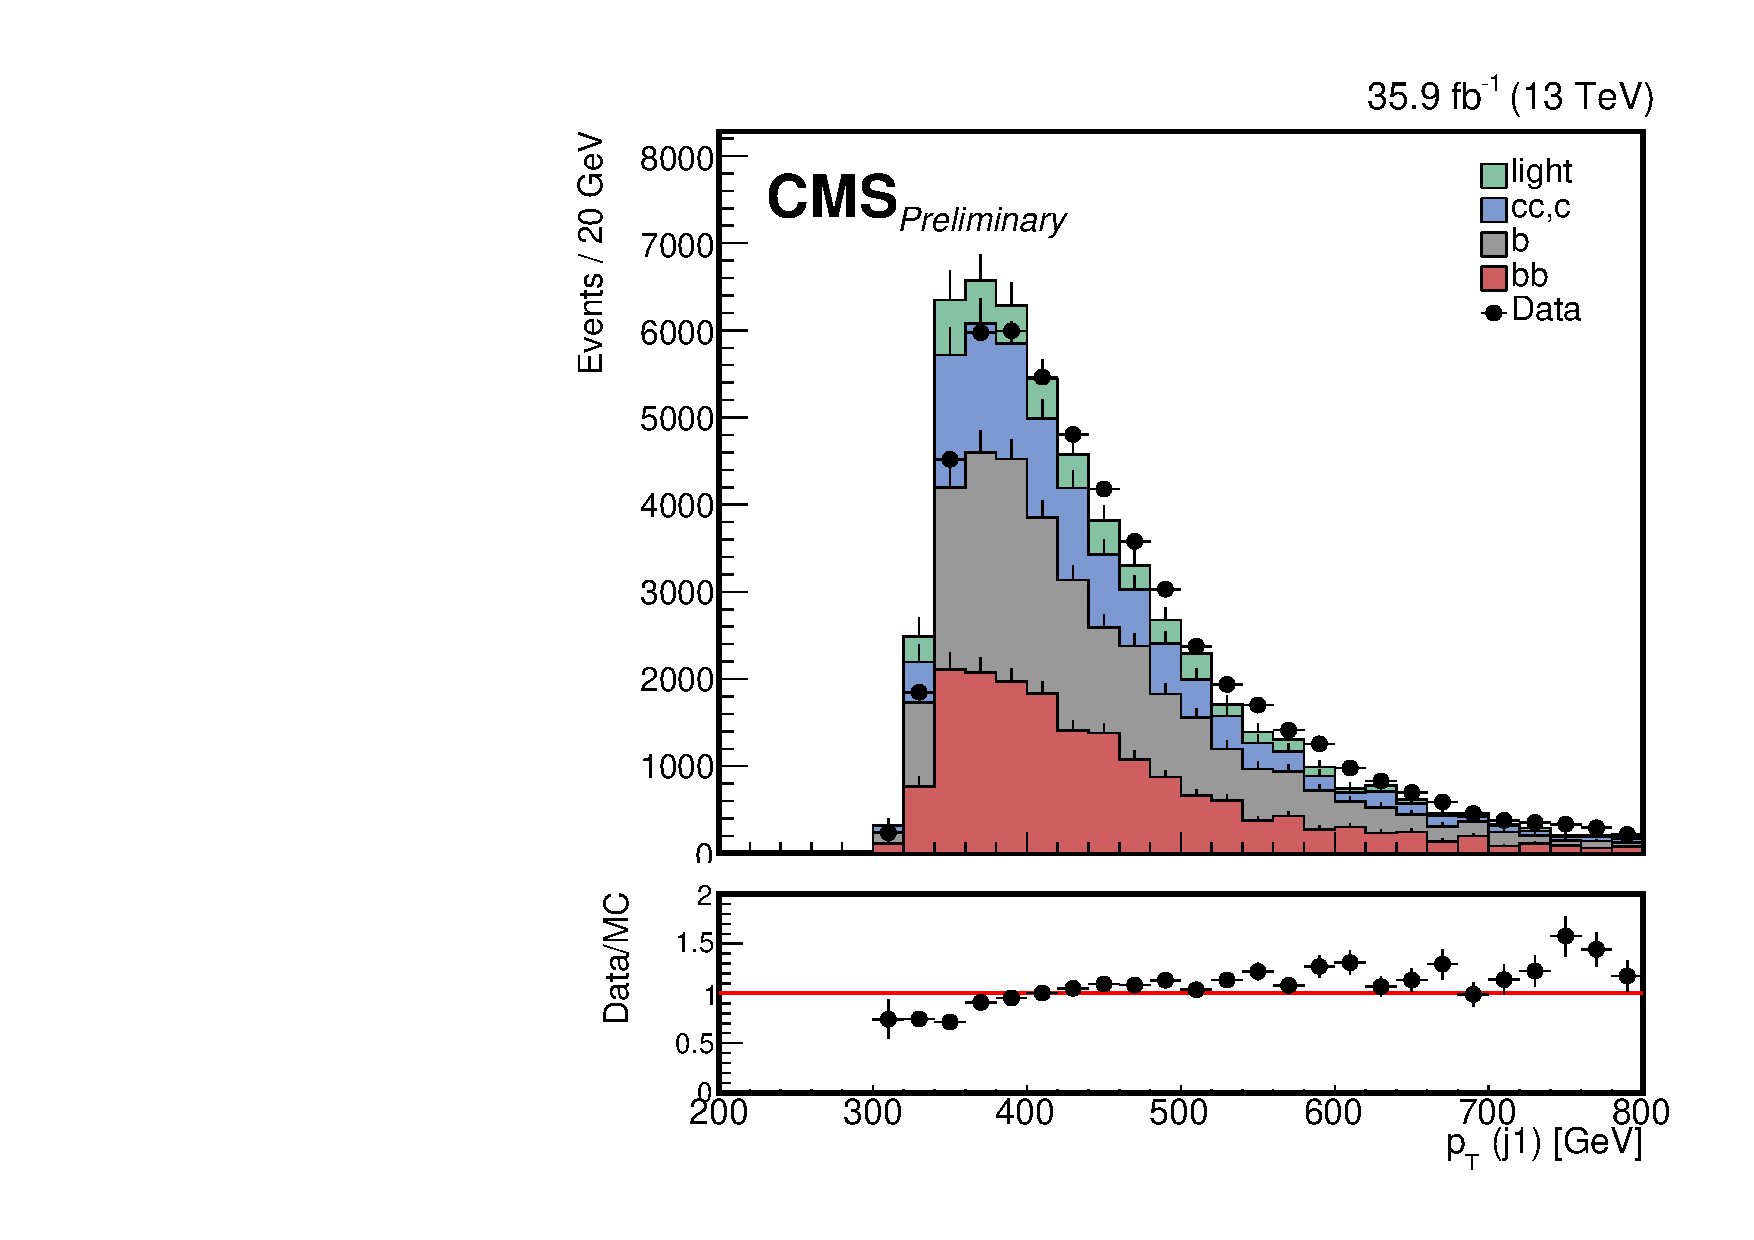
\includegraphics[width=0.5\textwidth]{Figures/dataMC_trig_antiTau21/pt_j0.pdf} &
    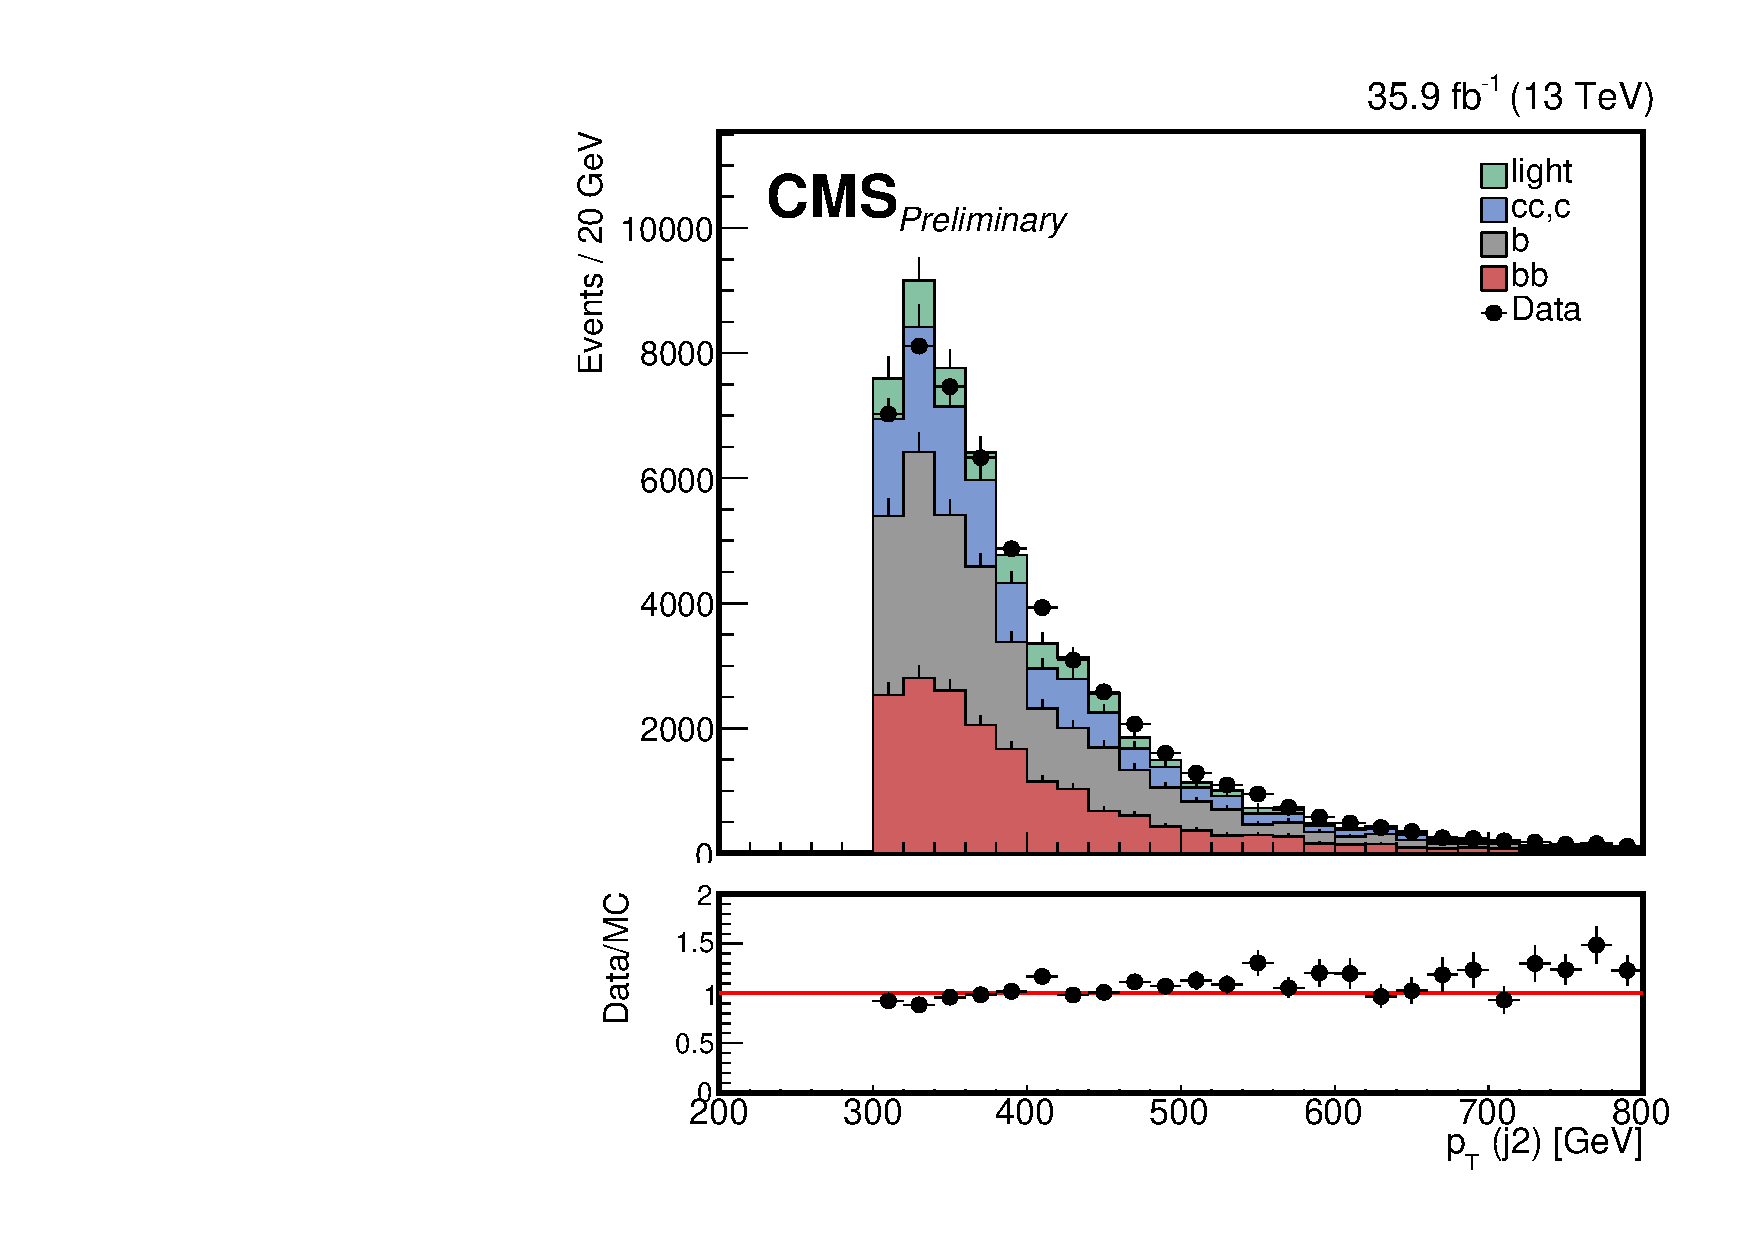
\includegraphics[width=0.5\textwidth]{Figures/dataMC_trig_antiTau21/pt_j1.pdf} \\
     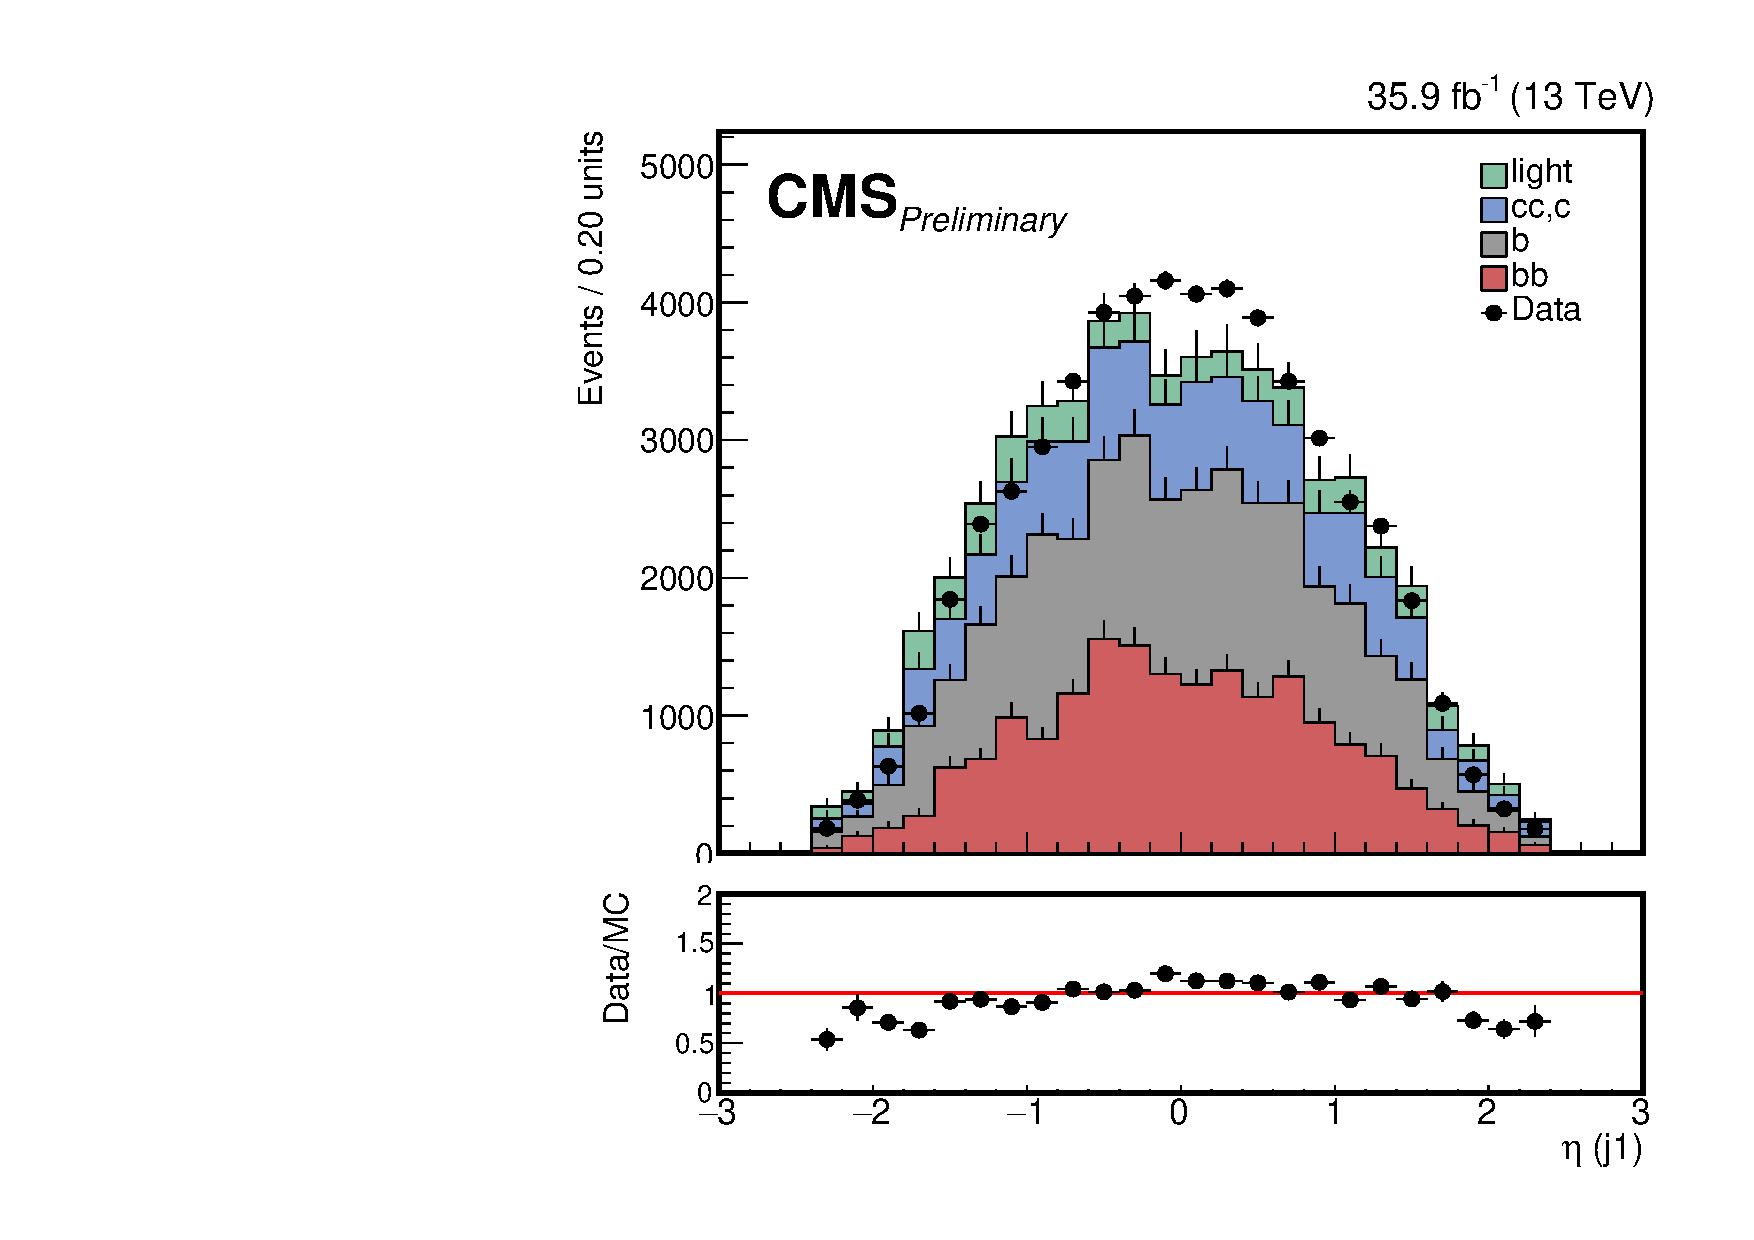
\includegraphics[width=0.5\textwidth]{Figures/dataMC_trig_antiTau21/eta_j0.pdf} &
    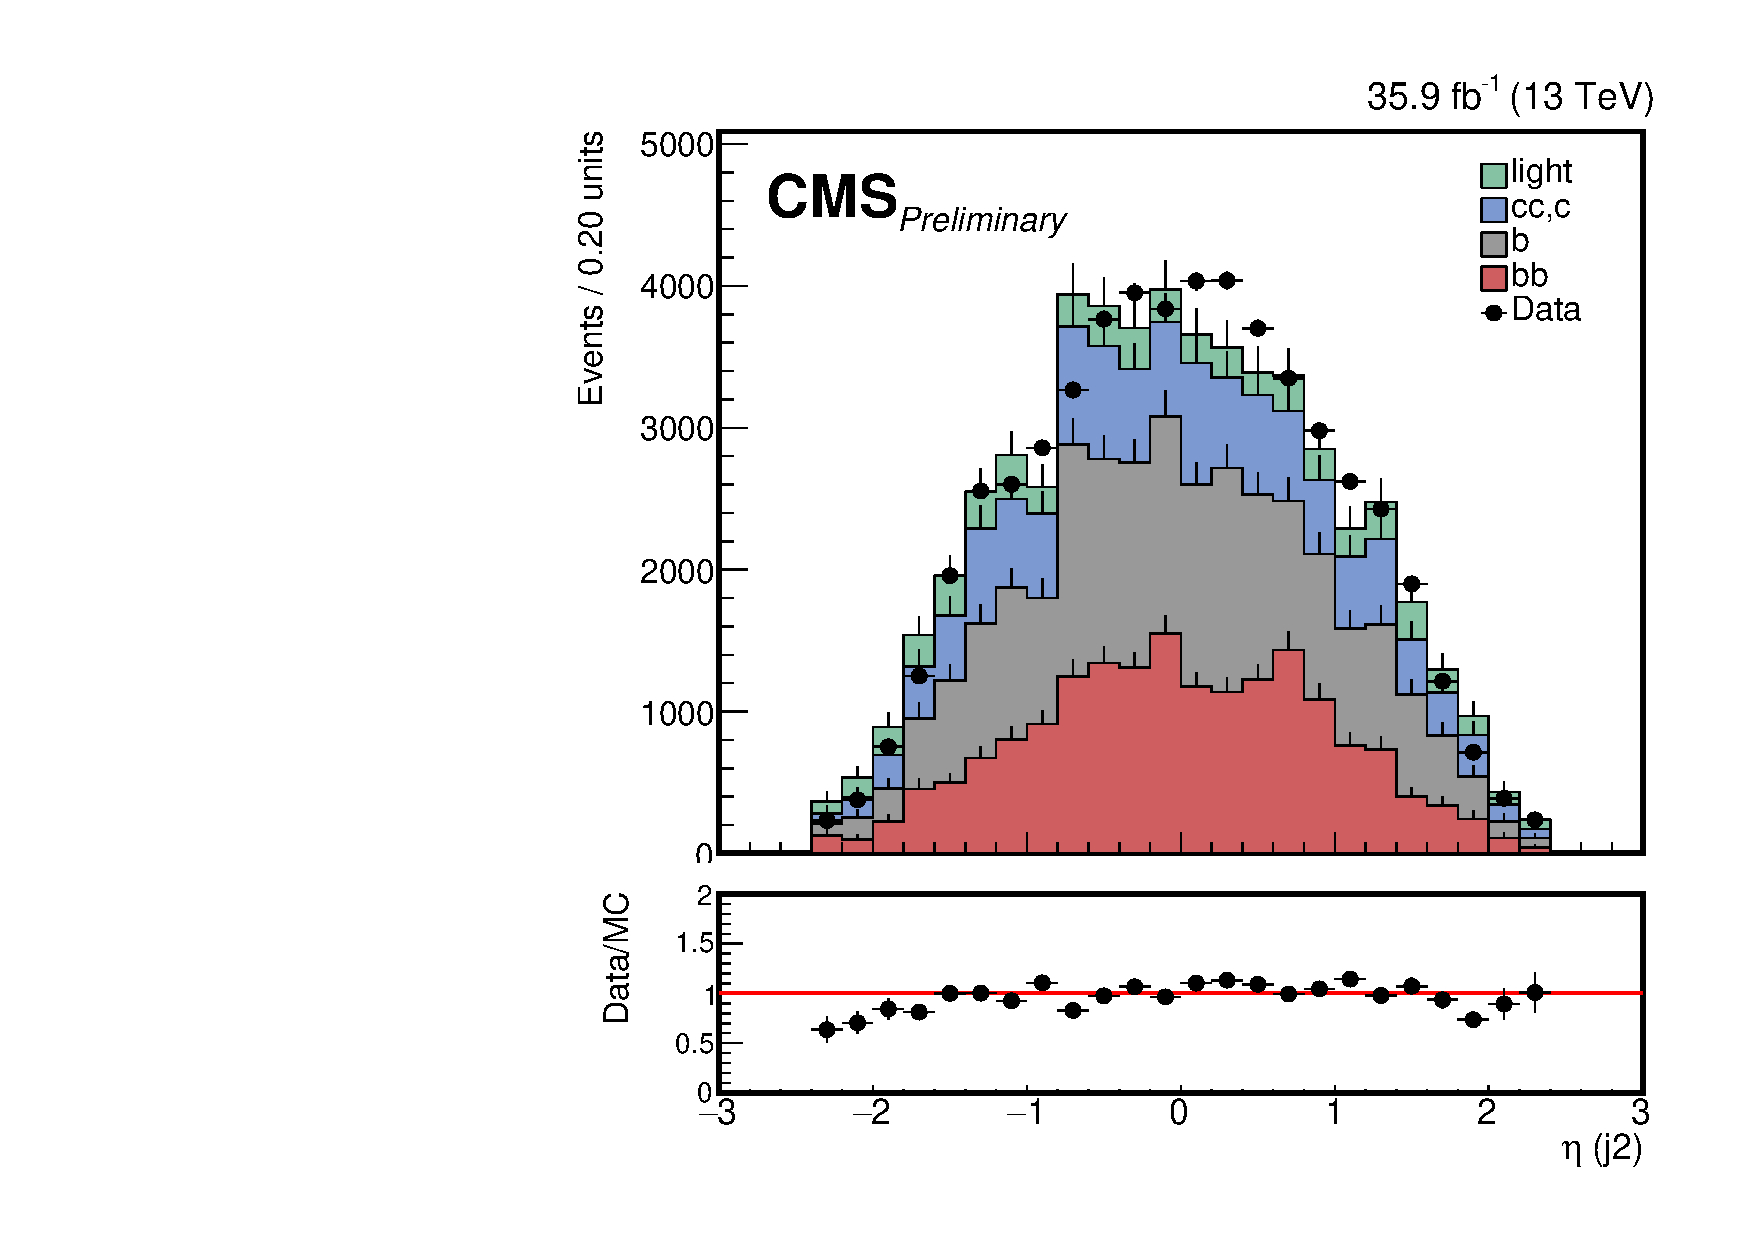
\includegraphics[width=0.5\textwidth]{Figures/dataMC_trig_antiTau21/eta_j1.pdf} \\
     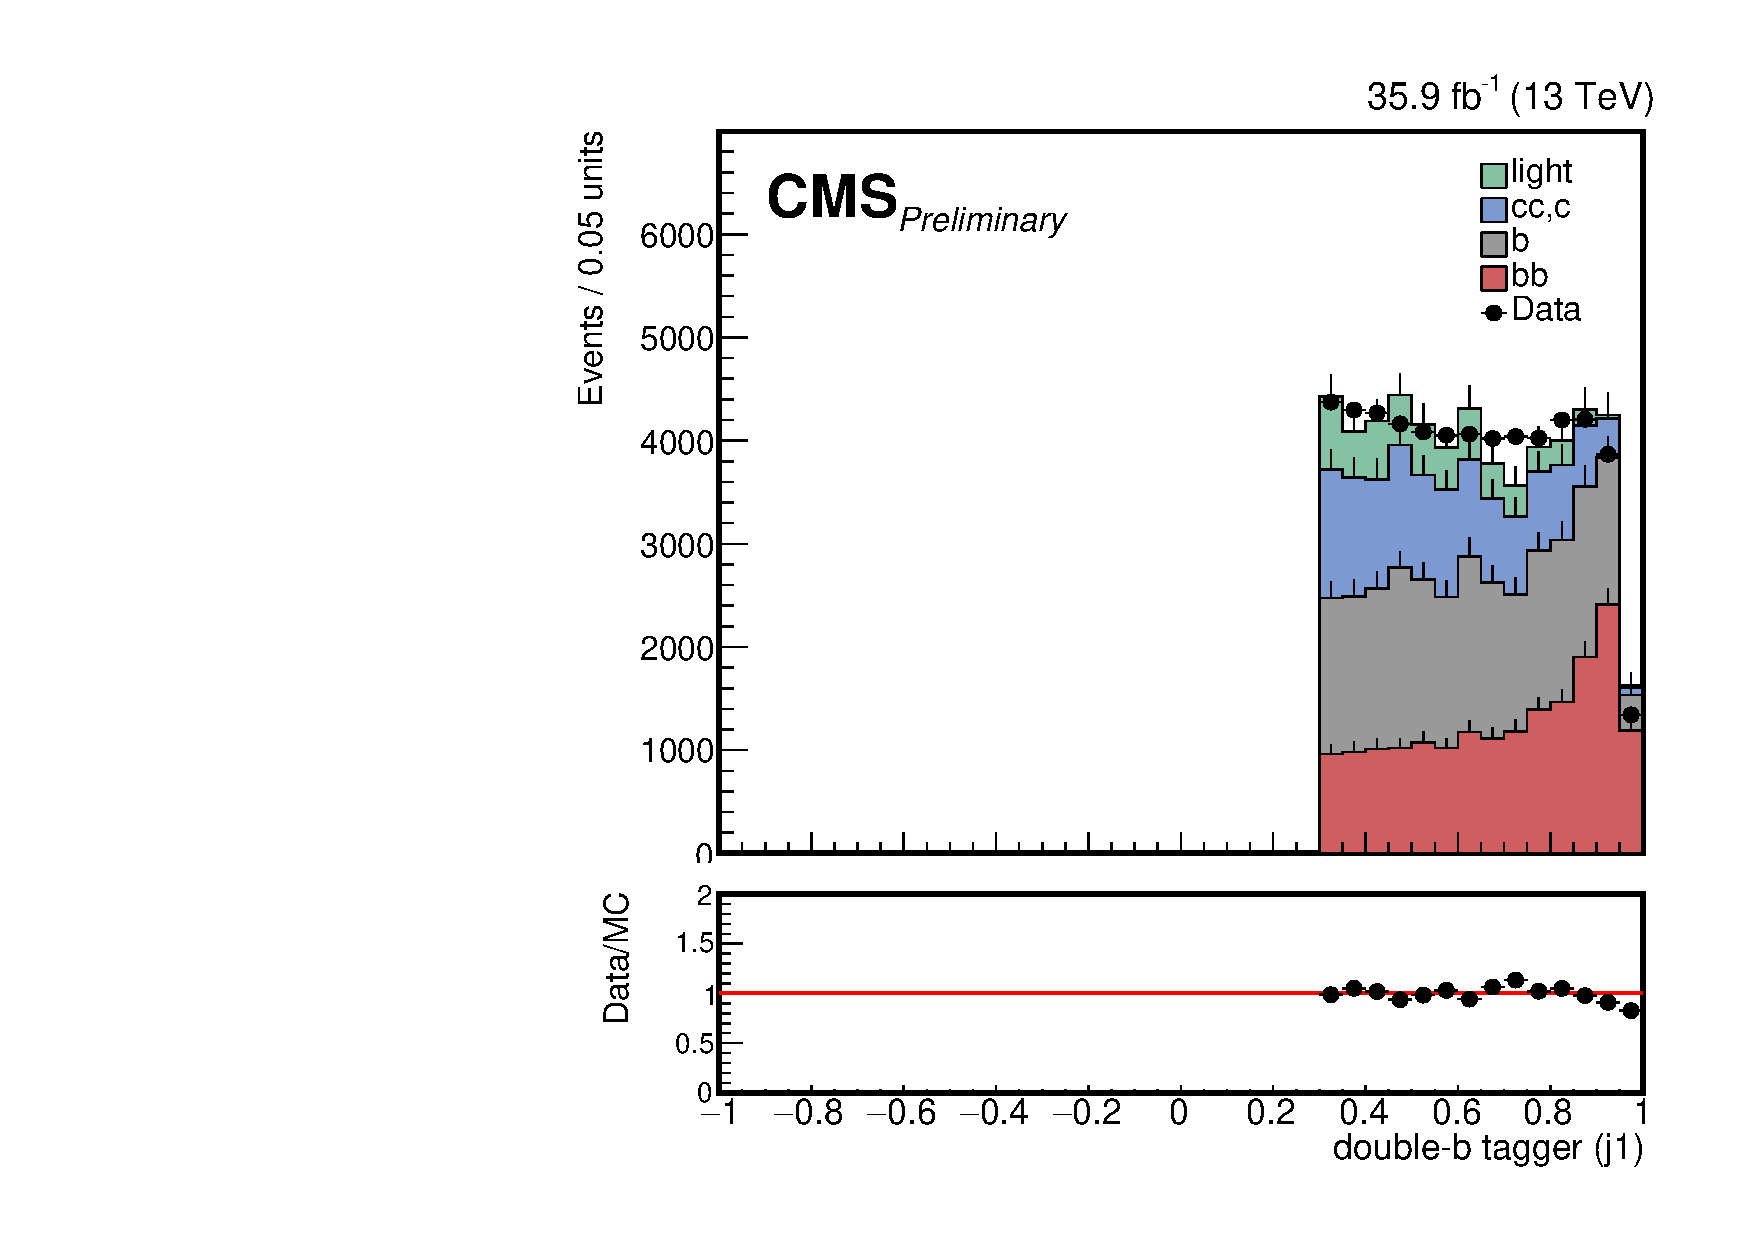
\includegraphics[width=0.5\textwidth]{Figures/dataMC_trig_antiTau21/doubleSV_j0.pdf} &
    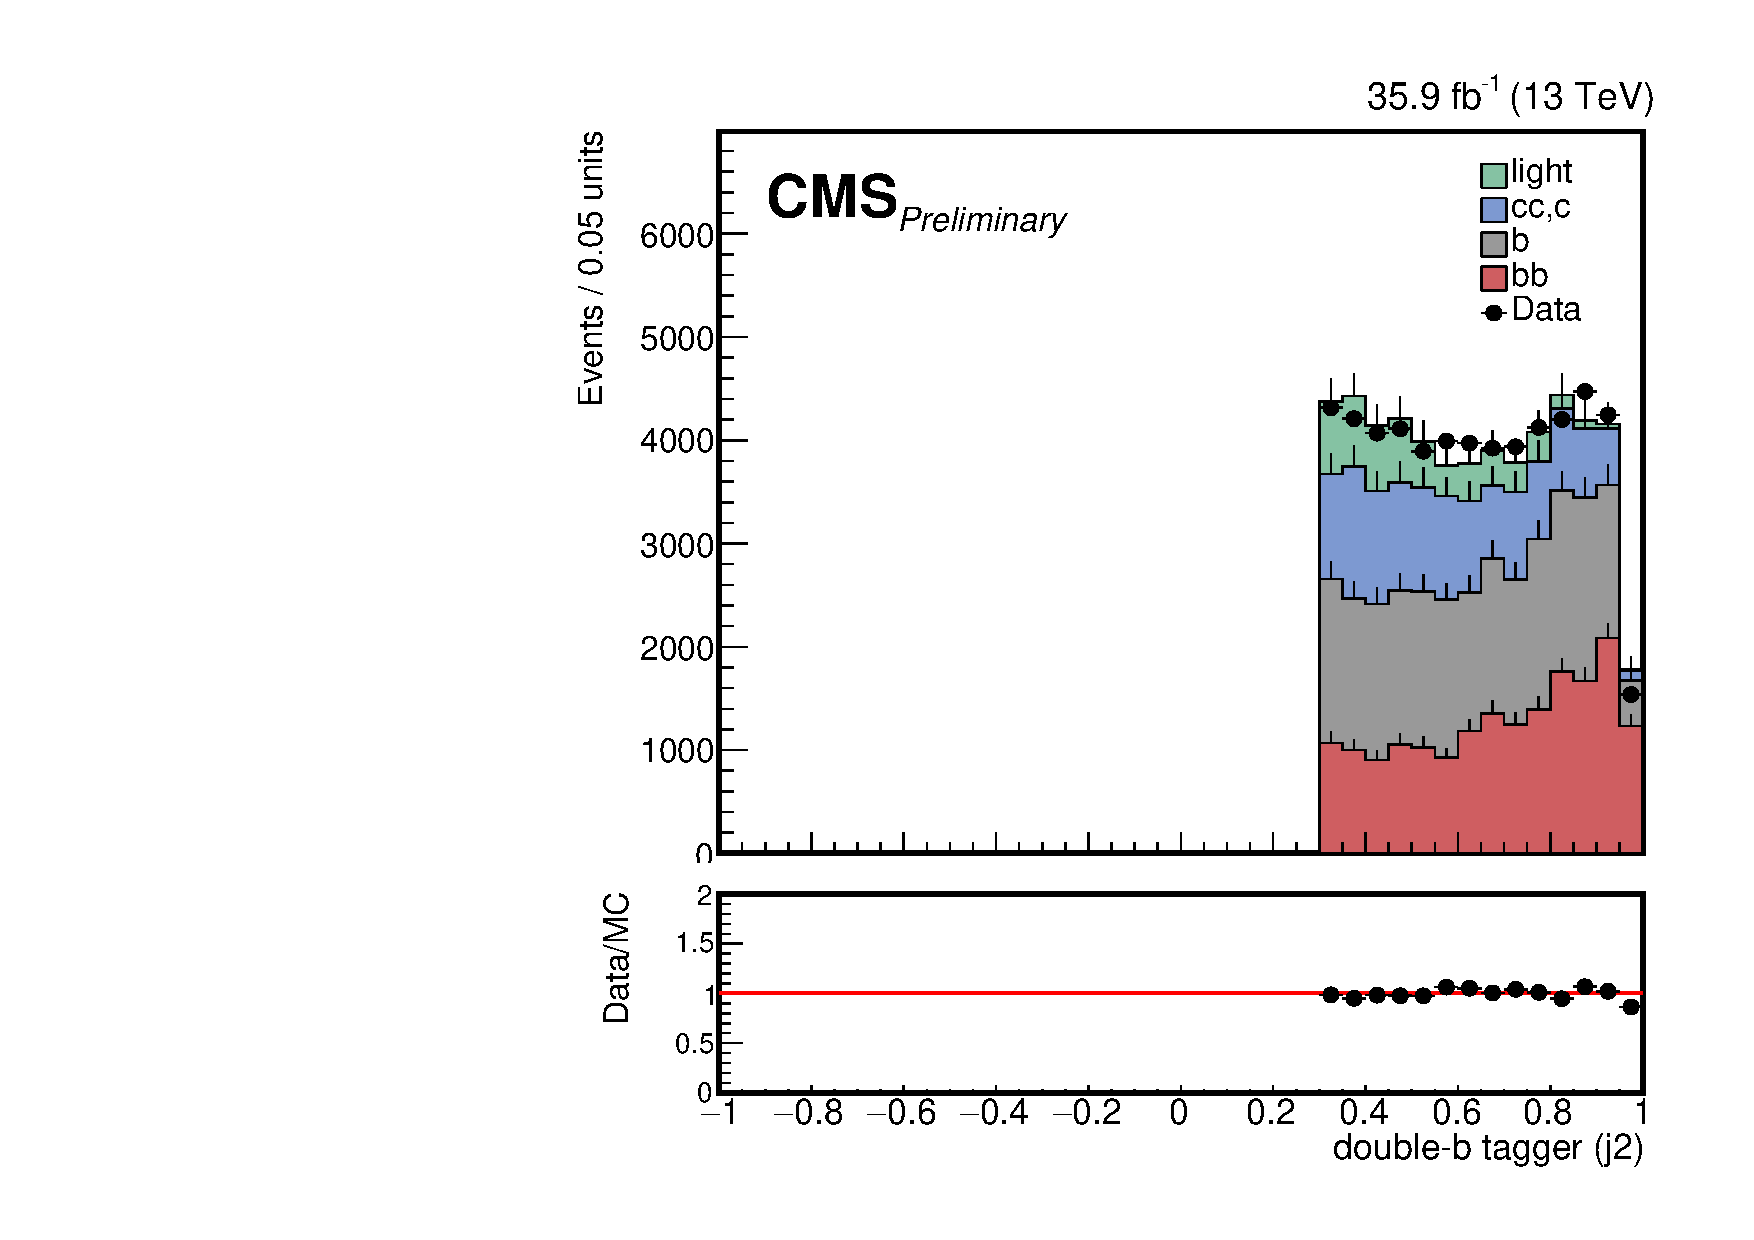
\includegraphics[width=0.5\textwidth]{Figures/dataMC_trig_antiTau21/doubleSV_j1.pdf} \\
  \end{tabular}
  \caption{The comparison of data and background in inverse $\tau _{21}$ region. Multi-jet events are seperated into four categories summarized in the table 3.10. From top to buttom are the comparison of $p_{T}$, $\eta $, and double-b tagger of leading (left) and next leading (right) AK8 jet.}
  \label{fig:hvt_brs}
\end{figure}
\begin{figure}[t]
  \centering
  \begin{tabular}{cc}
    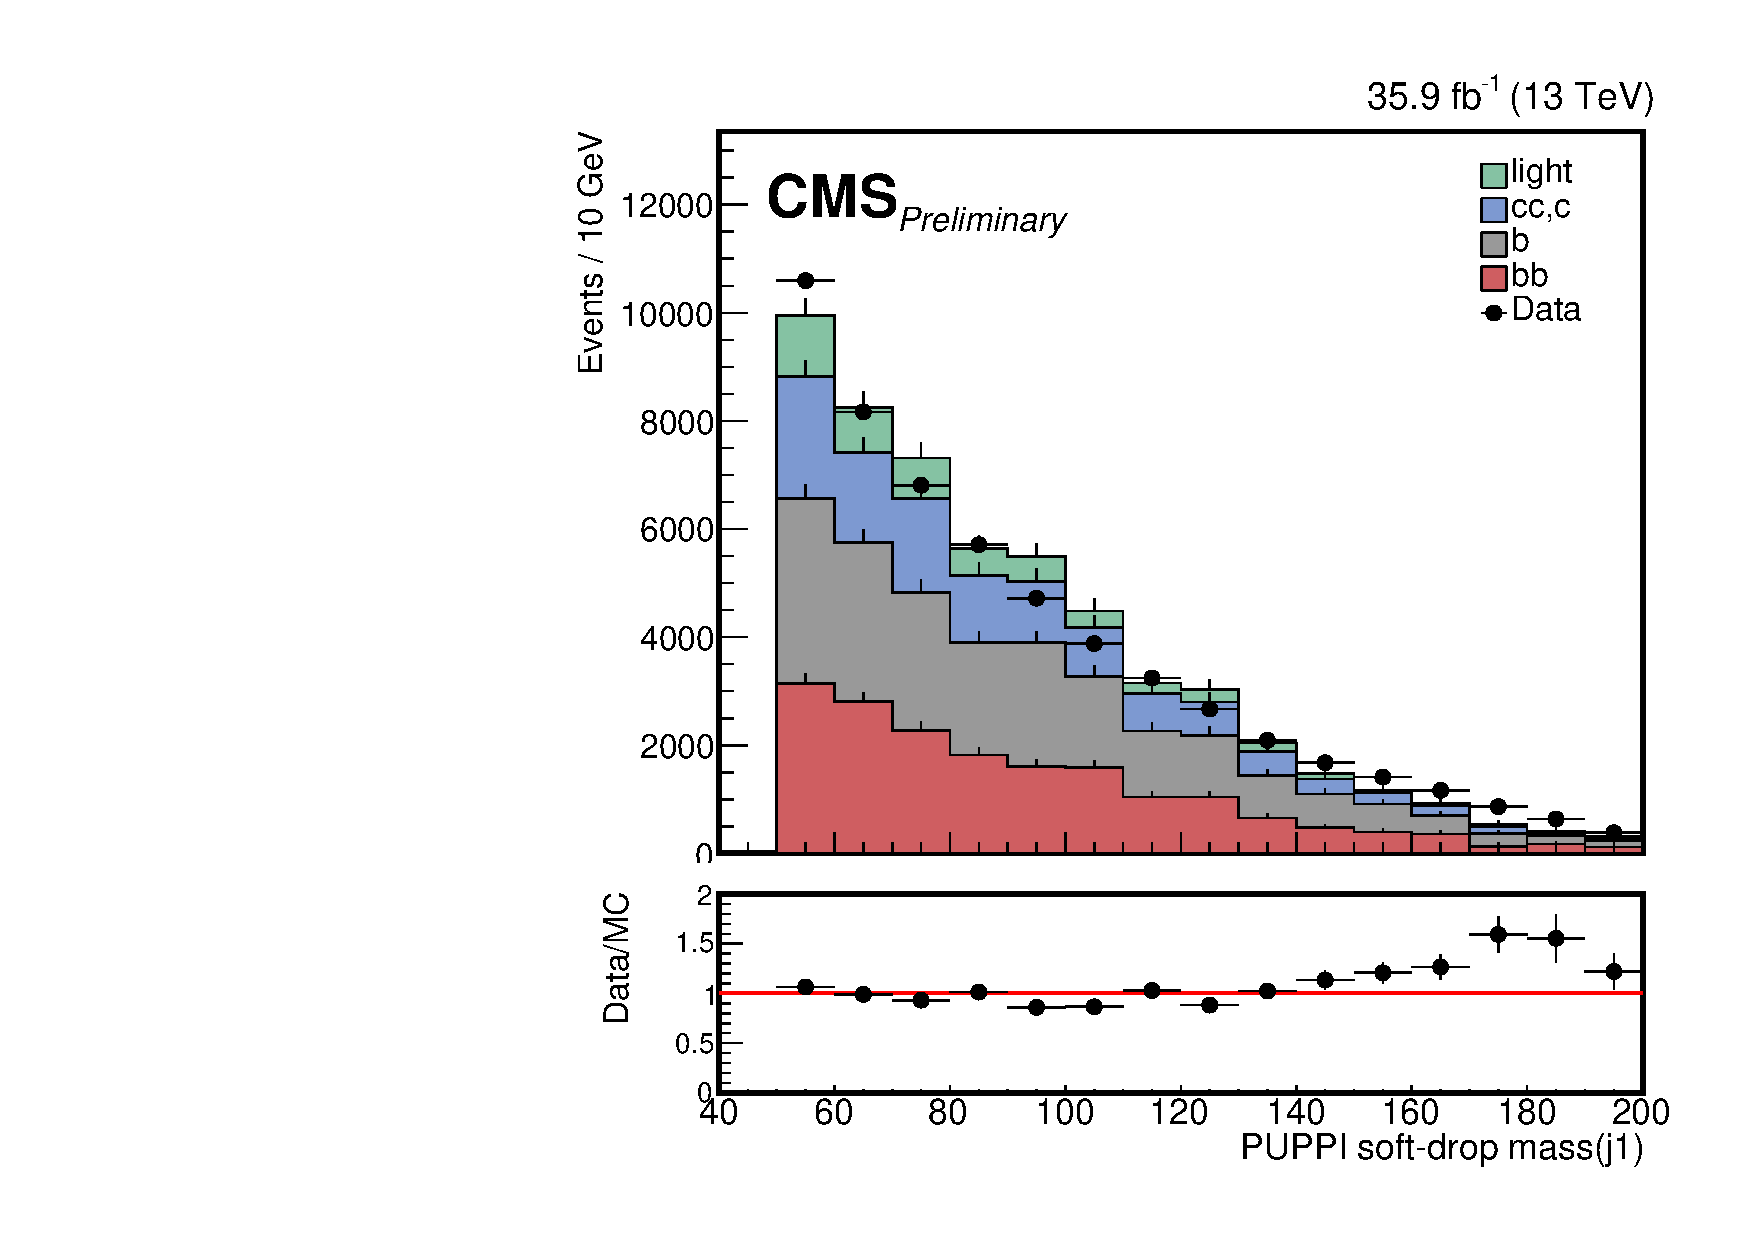
\includegraphics[width=0.5\textwidth]{Figures/dataMC_trig_antiTau21/puppiSDMassThea_j0.pdf} &
    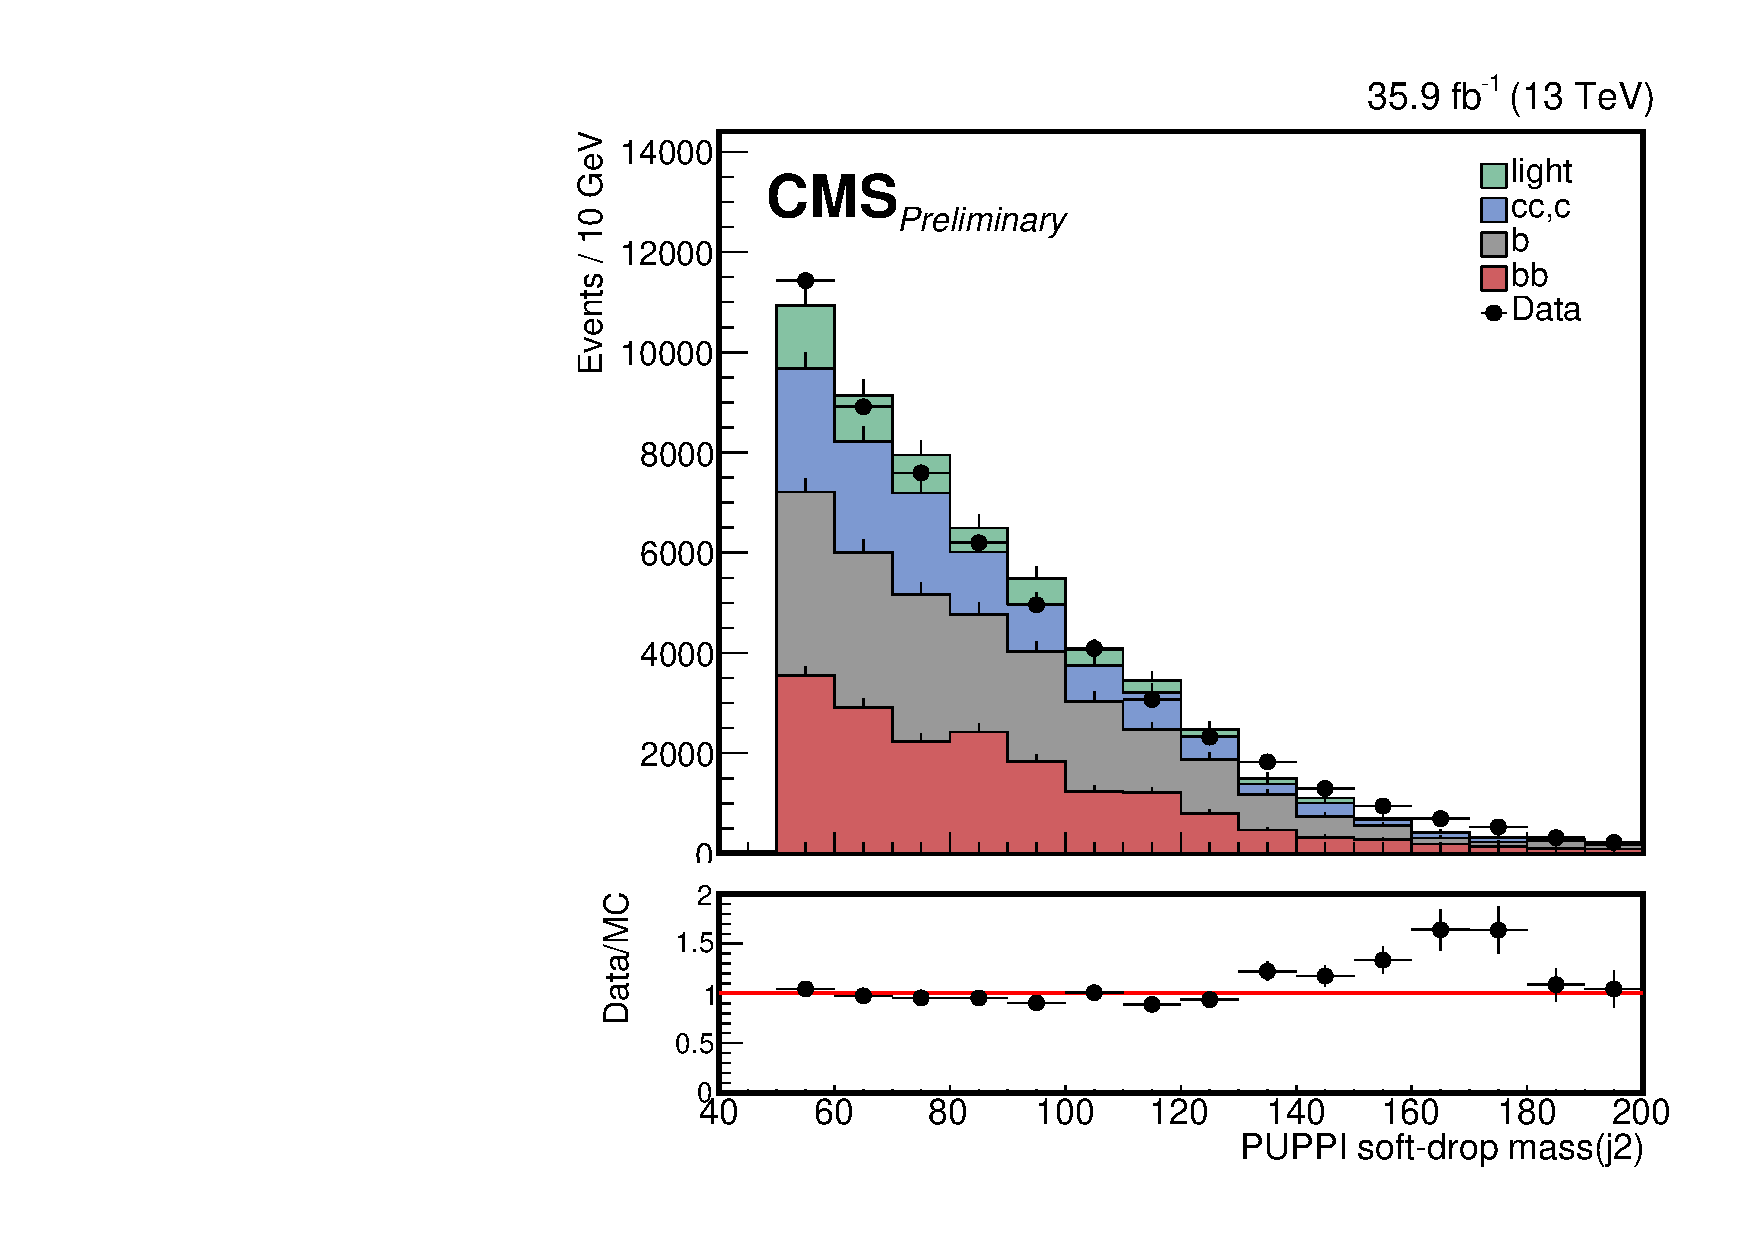
\includegraphics[width=0.5\textwidth]{Figures/dataMC_trig_antiTau21/puppiSDMassThea_j1.pdf} \\
     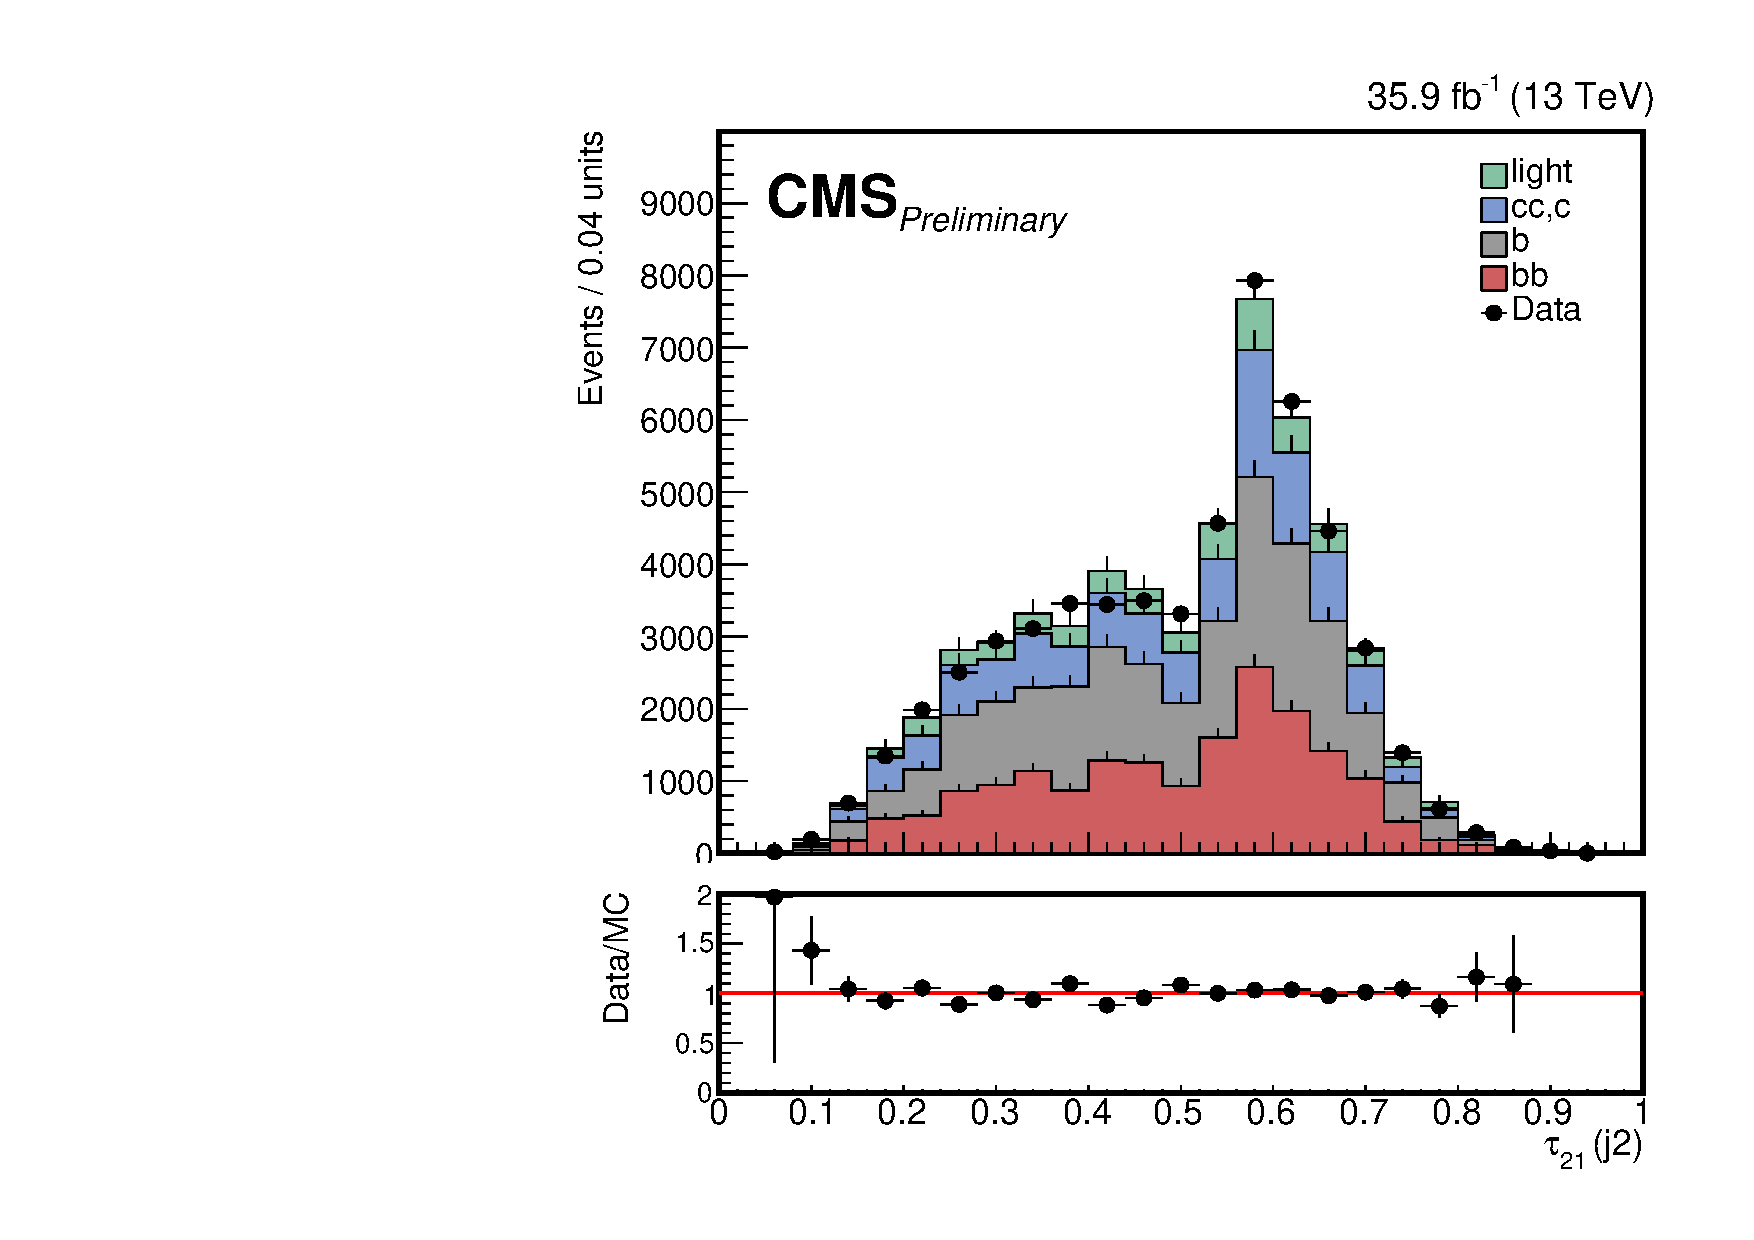
\includegraphics[width=0.5\textwidth]{Figures/dataMC_trig_antiTau21/puppiTau21_j0.pdf} &
    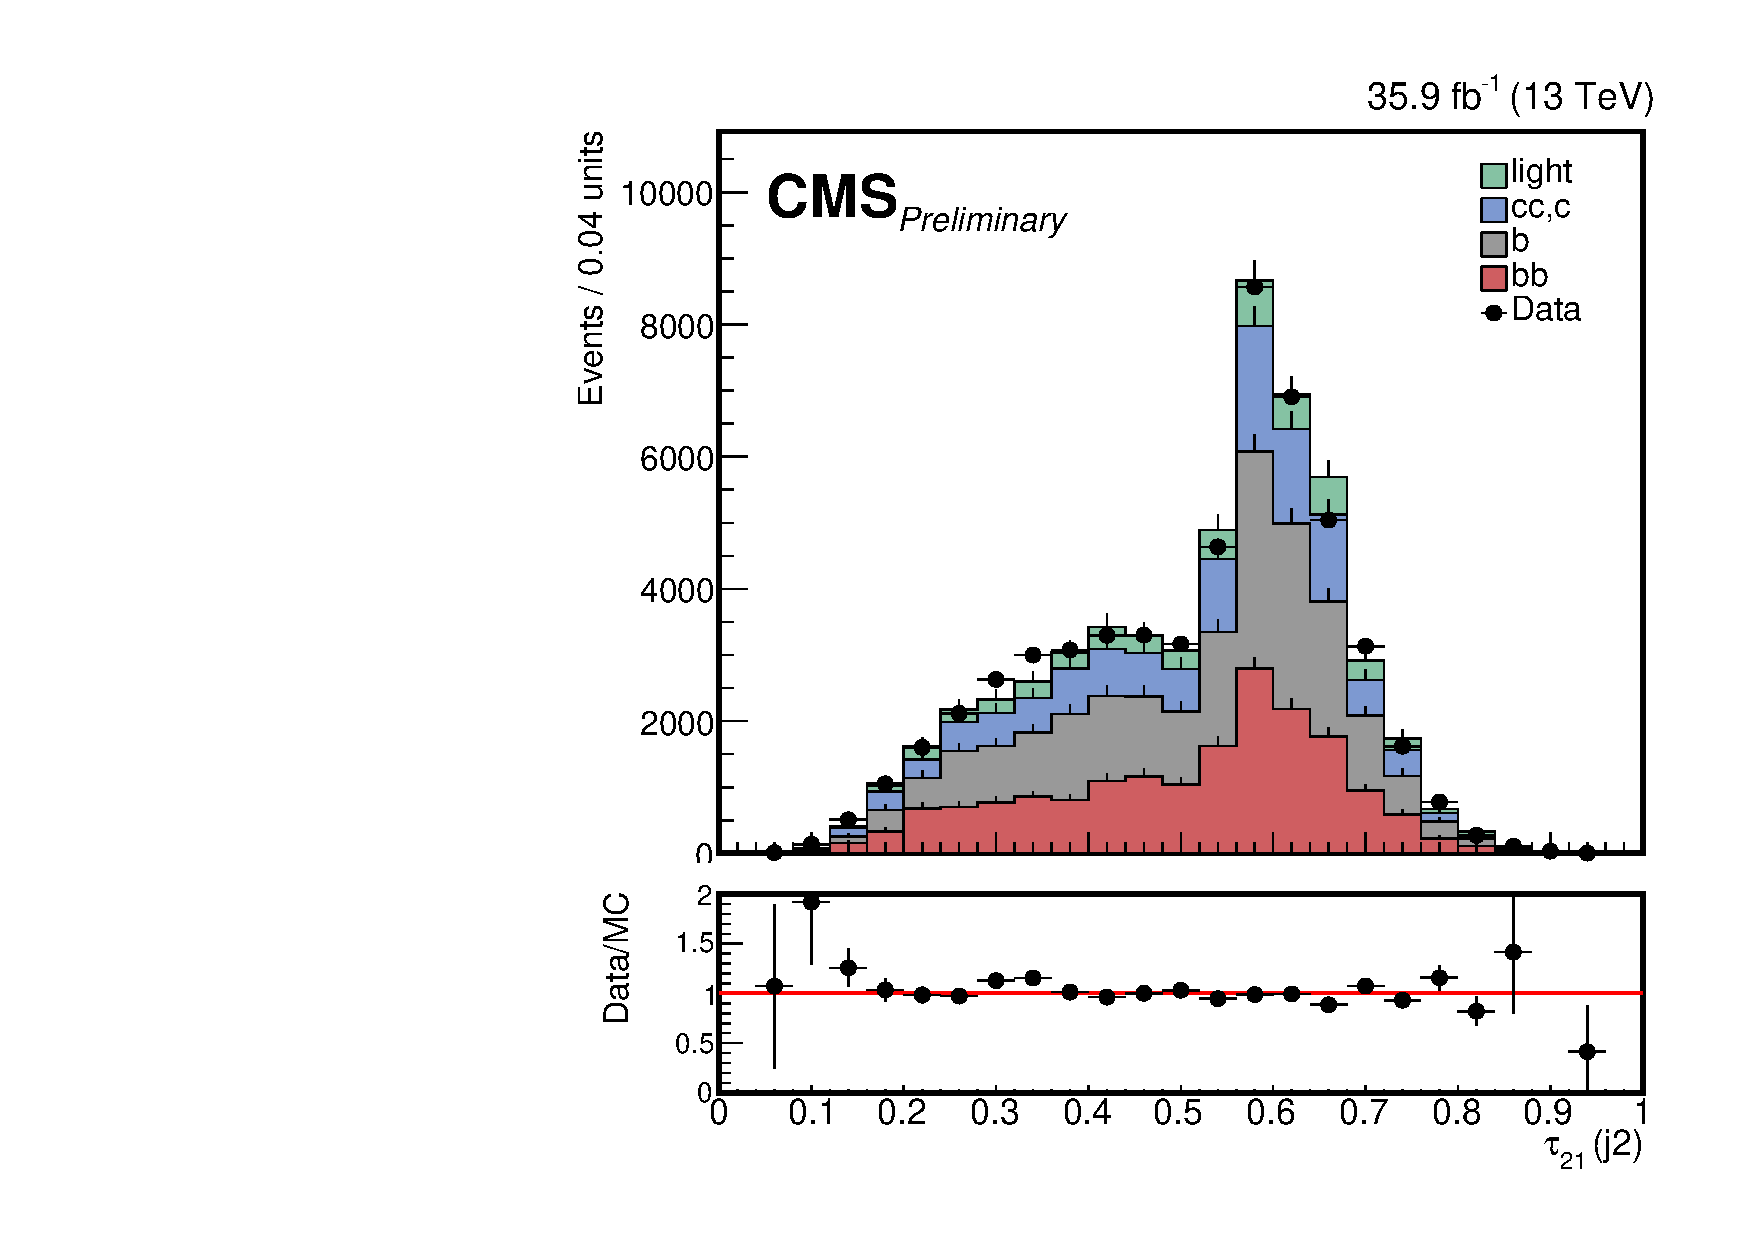
\includegraphics[width=0.5\textwidth]{Figures/dataMC_trig_antiTau21/puppiTau21_j1.pdf} \\
     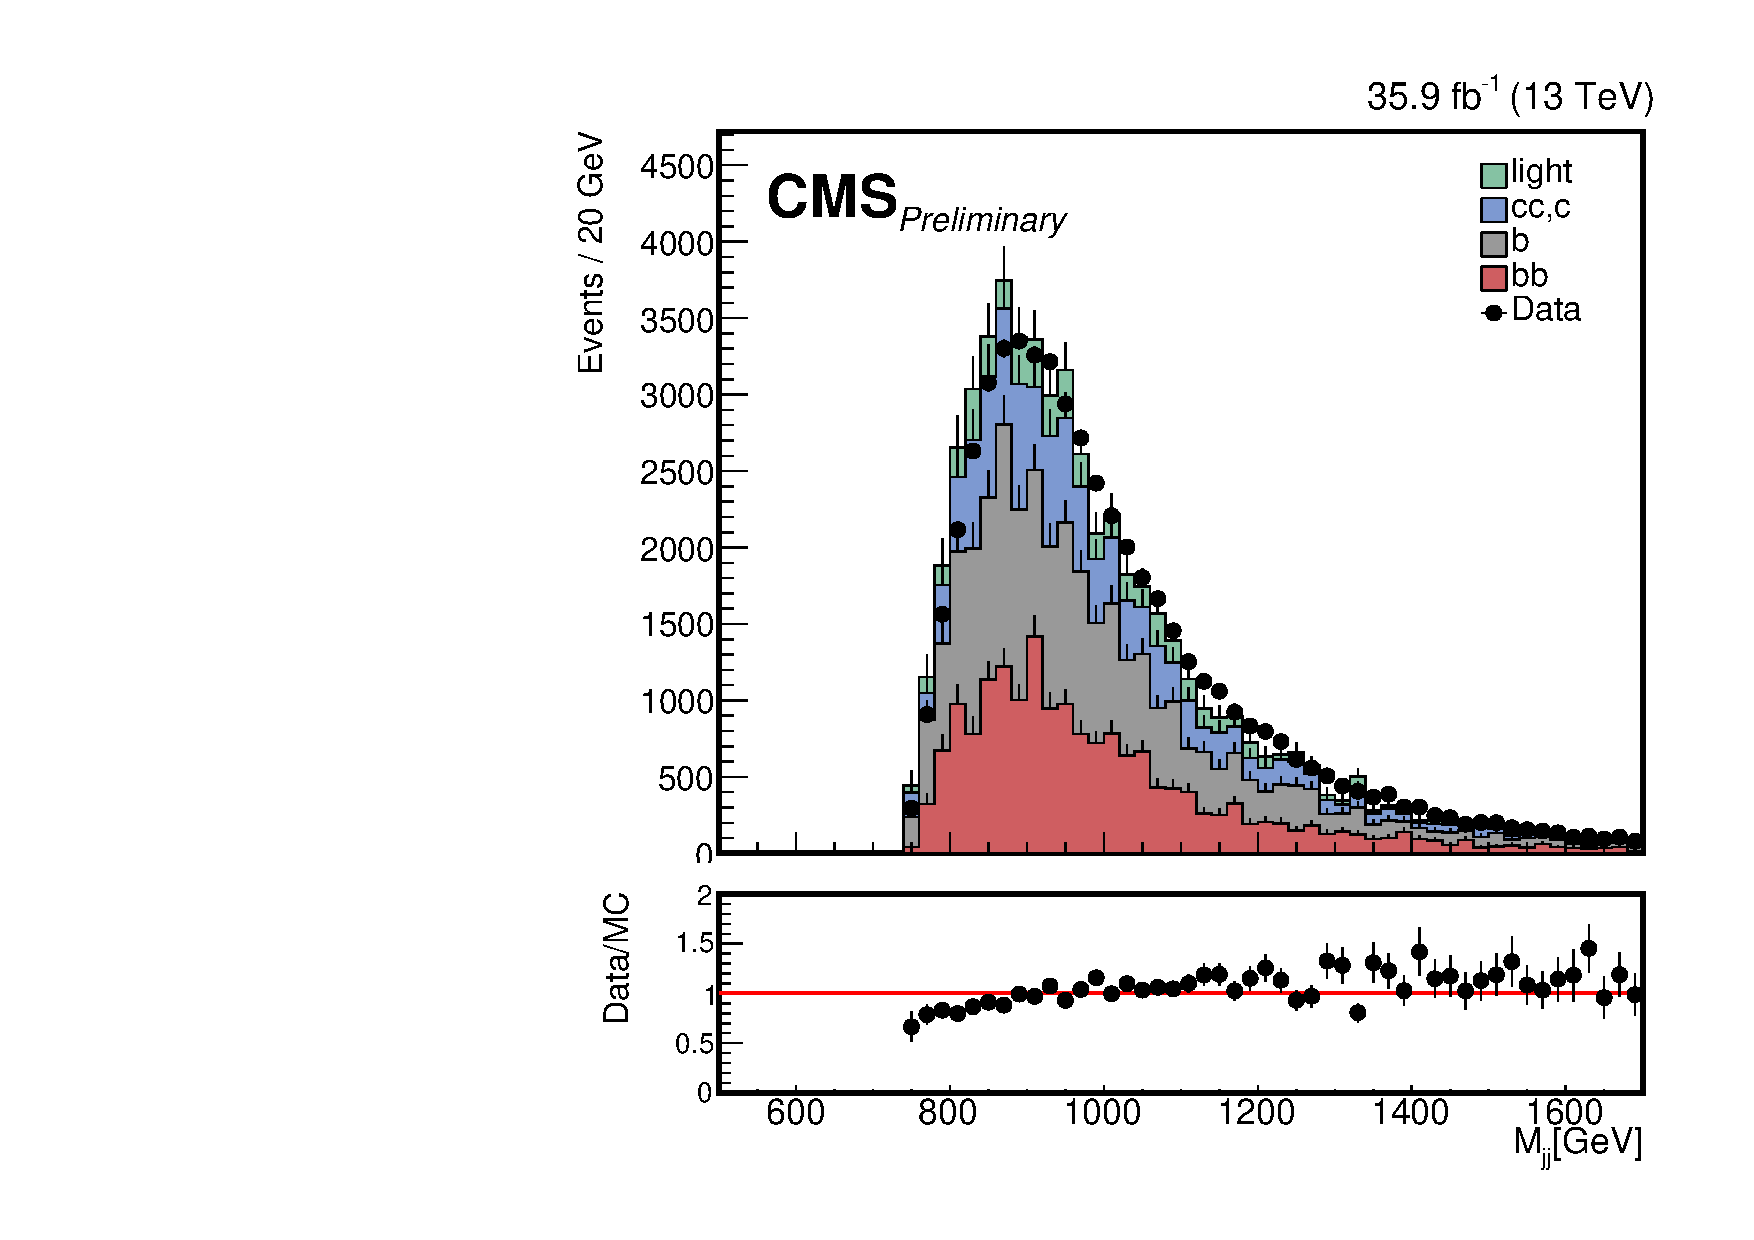
\includegraphics[width=0.5\textwidth]{Figures/dataMC_trig_antiTau21/totalMassRed.pdf} &
    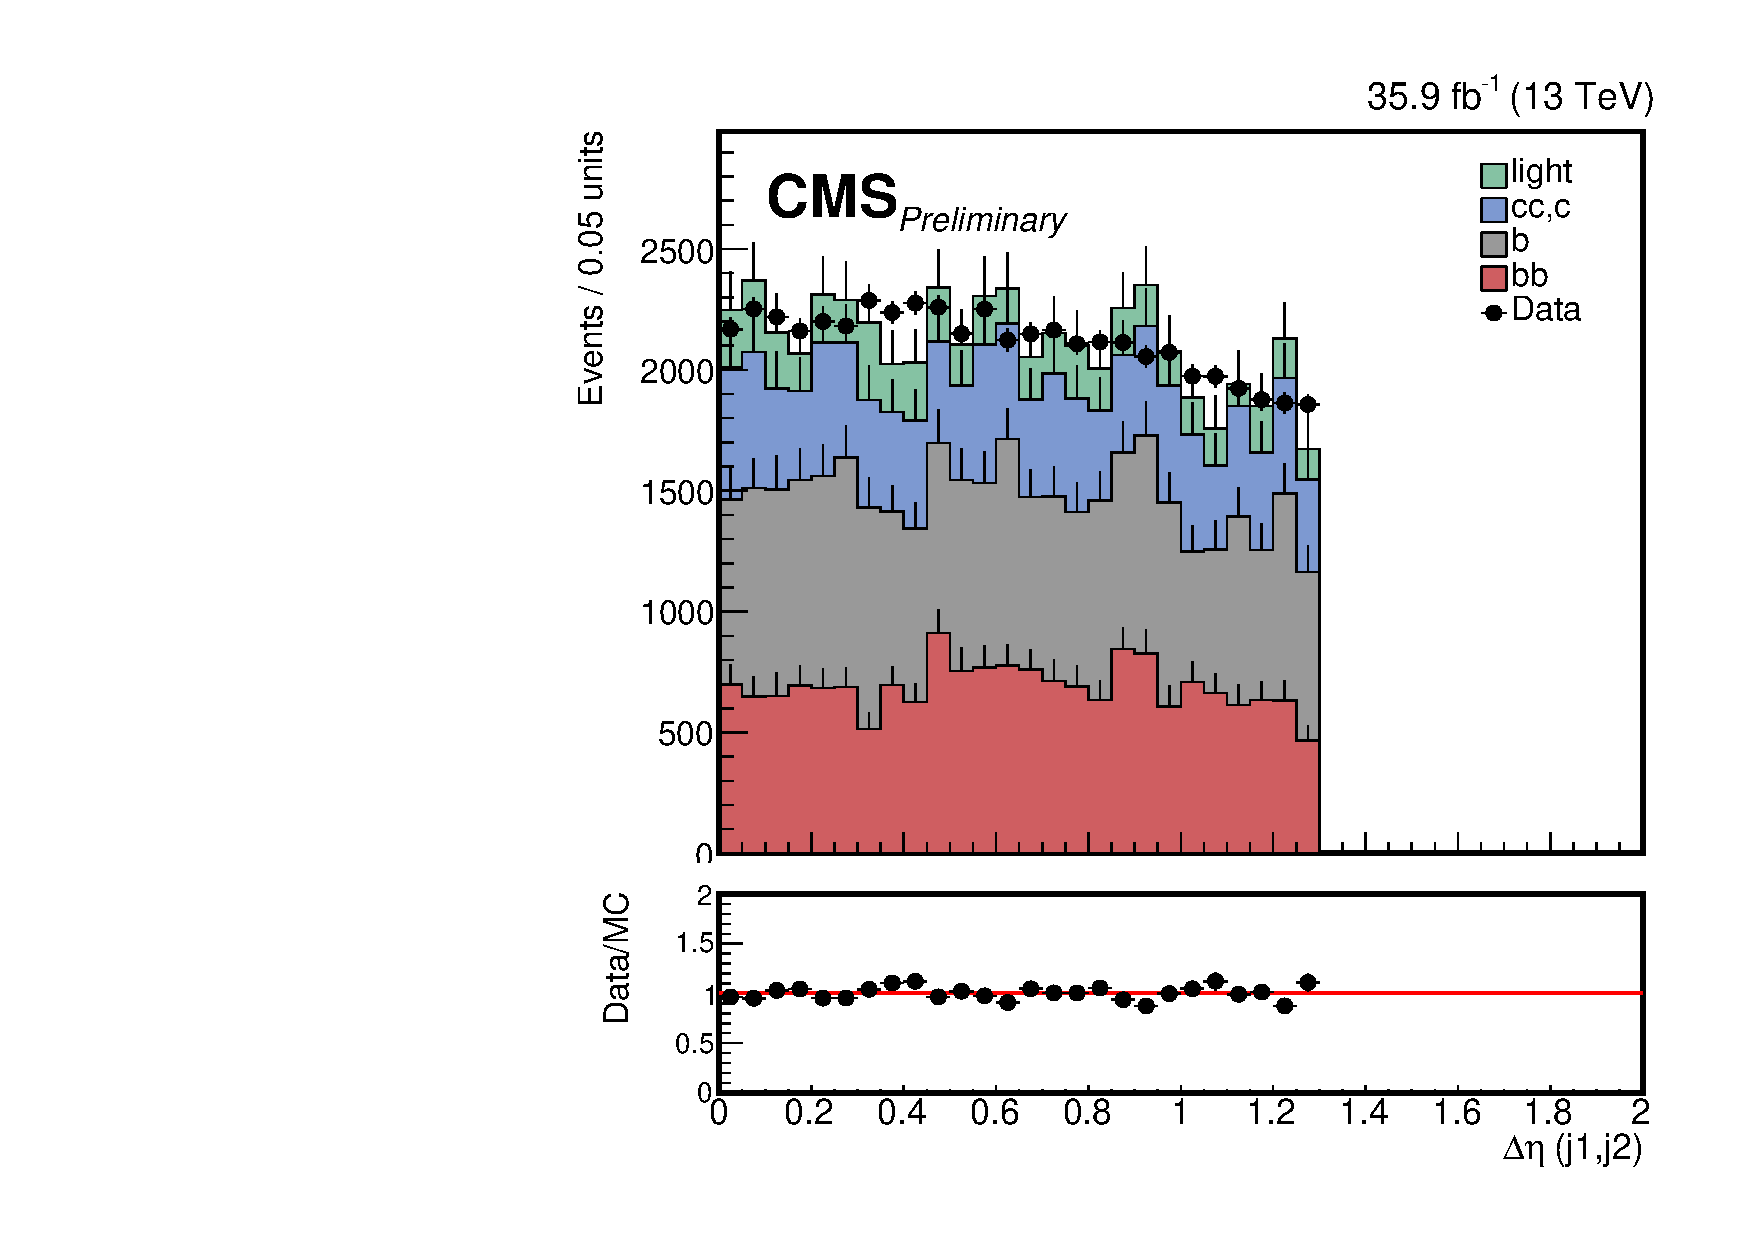
\includegraphics[width=0.5\textwidth]{Figures/dataMC_trig_antiTau21/deltaEta.pdf} \\
  \end{tabular}
  \caption{The comparison of data and background in inverse $\tau _{21}$ region. Multi-jet events are seperated into four categories summarized in the table 3.10. From top to buttom are the comparison of PUPPI soft-drop mass, $\tau _{21}$ of leading (left) and next leading (right) AK8 jet, the reduced mass (buttom left), and |$\Delta \eta $ (the two leading AK8 jets)| (buttom right).}
  \label{fig:hvt_brs}
\end{figure}
%For each distribution, all selection described in previous section is required except the variable itself and double-b tagger discriminant.  